\section{Hàm số liên tục}
\setcounter{dang}{0}
\subsection{Tóm tắt lý thuyết}
\begin{tomtat}
	\subsubsection{Hàm số liên tục tại một điểm}
	\begin{itemize}
		\item Cho hàm số $y=f(x)$ xác định trên khoảng $(a;b)$ chứa điểm $x_0$. Hàm số $f(x)$ được gọi là \textcolor{red}{liên tục tại điểm} $x_0$ nếu $\lim\limits_{x\to{x_0}}f(x)=f(x_0)$.
		\item Hàm số $f(x)$ không liên tục tại $x_0$ được gọi là \textcolor{red}{gián đoạn} tại điểm đó.
		\begin{note}
			Hàm số $y=f(x)$ liên tục tại $x_0$ khi và chỉ khi $\lim\limits_{x\to{x_0}^+}f(x)=\lim\limits_{x\to{x_0}^-}f(x)=f(x_0)$.
		\end{note}
	\end{itemize}
	\subsubsection{Hàm số liên tục trên một khoảng}
	\begin{itemize}
		\item Hàm số $y=f(x)$ được gọi là \textcolor{red}{liên tục trên khoảng} $(a;b)$ nếu nó liên tục tại mọi điểm thuộc khoảng này.
		\item Hàm số $y=f(x)$ được gọi là \textcolor{red}{liên tục trên đoạn} $[a;b]$ nếu nó liên tục trên khoảng $(a;b)$ và $\lim\limits_{x\to{a}^+}f(x)=f(a)$, $\lim\limits_{x\to{b}^-}f(x)=f(b)$.
		\item Các khái niệm hàm số liên tục trên nửa khoảng như $(a;b]$, $[a;+\infty)\ldots$ được định nghĩa theo cách tương tự.
		\item Đồ thị của hàm số liên tục trên một khoảng là một \textcolor{red}{đường liền nét} trên khoảng đó.
	\end{itemize}
	\subsubsection{Tính chất 1}
	\begin{itemize}
		\item Hàm số đa thức và các hàm số $y=\sin x$, $y=\cos x$ liên tục trên $\mathrm{R}$.
		\item Các hàm số $y=\tan x$, $y=\cot x$, $y=\sqrt x$ và các hàm phân thức hữu tỉ (thương của hai đa thức) liên tục trên mỗi khoảng xác định của chúng.
	\end{itemize}
	\subsubsection{Tính chất 2}
	Giả sử hai hàm số $y=f(x)$ và $y=g(x)$ liên tục tại điểm $x_0$. Khi đó:
	\begin{itemize}
		\item Các hàm số $y=f(x)+g(x)$, $y=f(x)-g(x)$ và $y=f(x)\cdot g(x)$ liên tục tại $x_0$.
		\item Hàm số $\dfrac{f(x)}{g(x)}$ liên tục tại $x_0$ nếu $g(x_0)\ne 0$.
	\end{itemize}
\end{tomtat}
\subsection{Các dạng toán thường gặp}
\begin{dang}{Dựa vào đồ thị xét tính liên tục của hàm số tại một điểm, một khoảng.}
	Để xét tính liên tục của hàm số khi biết đồ thị, ta cần nhớ:
	\begin{itemize}
		\item Đồ thị của hàm số liên tục trên một khoảng là một đường liền nét trên khoảng đó.
		\item Hàm số $y=f(x)$ liên tục tại $x_0$ khi và chỉ khi $\lim\limits_{x\to{x_0}^+}f(x)=\lim\limits_{x\to{x_0}^-}f(x)=f(x_0)$.
	\end{itemize}
\end{dang}
\subsubsection{Ví dụ mẫu}
\begin{vd}%[DCHT Toán 11 - KNTT -Vũ Hồng Toàn]%[1K5YG-2]
	\immini{
		Cho hàm số $y=f(x)$ có đồ thị như hình vẽ bên.\\ Xét tính liên tục của hàm số $y=f(x)$ trên khoảng $(0;2)$.	
	}
	{
		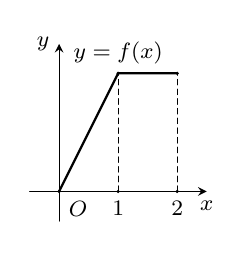
\begin{tikzpicture}[scale=.75, font=\footnotesize, line join=round, line cap=round,>=stealth]
			\def\xmin{-.5} \def\xmax{2.5}
			\def\ymin{-0.5} \def\ymax{2.5}
			\draw[->] (\xmin,0)--(0,0)node [below right]{$O$}-- (\xmax,0) node [below]{$x$};
			\draw[->] (0,\ymin)--(0,\ymax) node [left]{$y$};
			\draw[ thick] (0,0)--(1,2)--(2,2);
			\draw[dash pattern=on 2pt off 1.5pt] (1,0)node[below]{$1$}--(1,2) (2,0)node[below]{$2$}--(2,2)  (1,2)node[above ]{$y=f(x)$};
			\foreach \x/\y in{0/0,1/0,2/0,1/2,2/2} \fill(\x,\y)circle(.03);
		\end{tikzpicture}		
	}
	% \dapso{Hàm số liên tục trên khoảng $(0;2)$.}
	\loigiai{
		Đồ thị hàm số là một đường liền nét trên khoảng $(0;2)$ nên hàm số đã cho liên tục trên khoảng $(0;2)$.}
\end{vd}
\begin{vd}%[DCHT Toán 11 - KNTT -Vũ Hồng Toàn]%[1K5YG-2]
	\immini{
		Cho hàm số $y=f(x)$ có đồ thị như hình vẽ bên.\\ Xét tính liên tục của hàm số $y=f(x)$ trên khoảng $(-2;2)$.	
	}
	{
		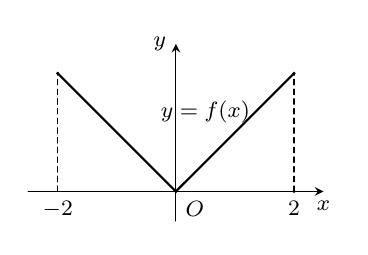
\begin{tikzpicture}[scale=.75, font=\footnotesize, line join=round, line cap=round,>=stealth]
			\def\xmin{-2.5} \def\xmax{2.5}
			\def\ymin{-0.5} \def\ymax{2.5}
			\draw[->] (\xmin,0)--(0,0)node [below right]{$O$}-- (\xmax,0) node [below]{$x$};
			\draw[->] (0,\ymin)--(0,\ymax) node [left]{$y$};
			\draw[ thick] plot[domain=-2:2](\x,{abs(\x)});
			\draw[dash pattern=on 2pt off 1.5pt] (-2,0)node[below]{$-2$}--(-2,2) (2,0)node[below]{$2$}--(2,2)  (.5,1)node[above ]{$y=f(x)$};
			\foreach \x/\y in{0/0,2/0,-2/2,2/2} \fill(\x,\y)circle(.03);
		\end{tikzpicture}		
	}
	% \dapso{Hàm số liên tục trên khoảng $(-2;2)$.}
	\loigiai{
		Đồ thị hàm số là một đường liền nét trên khoảng $(-2;2)$ nên hàm số đã cho liên tục trên khoảng $(-2;2)$.}
\end{vd}

\begin{vd}%[DCHT Toán 11 - KNTT -Vũ Hồng Toàn]%[1K5BG-2]
	\immini{
		Cho hàm số $y=f(x)$ có đồ thị như hình vẽ bên.\\ Xét tính liên tục của hàm số $y=f(x)$ trên khoảng $(0;2)$.	
	}
	{
		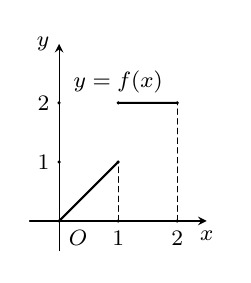
\begin{tikzpicture}[scale=.75, font=\footnotesize, line join=round, line cap=round,>=stealth]
			\def\xmin{-.5} \def\xmax{2.5}
			\def\ymin{-0.5} \def\ymax{3}
			\draw[->] (\xmin,0)--(0,0)node [below right]{$O$}-- (\xmax,0) node [below]{$x$};
			\draw[->] (0,\ymin)--(0,\ymax) node [left]{$y$};
			\draw[ thick] (0,0)--(1,1) (1,2)--(2,2);
			\draw[dash pattern=on 2pt off 1.5pt] (1,0)node[below]{$1$}--(1,1) (2,0)node[below]{$2$}--(2,2) (0,1)node[left]{$1$} (0,2)node[left]{$2$}
			(1,2)node[above ]{$y=f(x)$}
			;
			\foreach \x/\y in{0/0,1/0,2/0,1/2,2/2,1/1,0/1,0/2} \fill(\x,\y)circle(.03);
		\end{tikzpicture}		
	}
	
	% \dapso{Hàm số đã cho liên tục trên các khoảng $(0,1)$, $(1,2)$ và gián đoạn tại $x=1$.}
	\loigiai{
		\begin{itemize}
			\item Đồ thị hàm số là các đường liền nét trên các khoảng $(0;1)$, $(1;2)$ do đó hàm số liên tục trên các khoảng này.
			\item Đồ thị hàm số không liền nét tại điểm $x=1$ do đó hàm số đã cho gián đoạn tại điểm này.
		\end{itemize}
	}
\end{vd}
\begin{vd}%[DCHT Toán 11 - KNTT -Vũ Hồng Toàn]%[1K5BG-2]
	\immini{
		Cho hàm số $y=f(x)$ có đồ thị như hình vẽ bên.\\ Xét tính liên tục của hàm số $y=f(x)$ trên khoảng $(0;2)$.	
	}
	{
		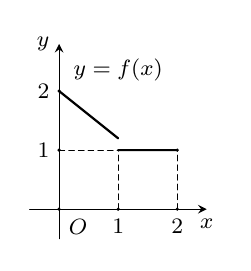
\begin{tikzpicture}[scale=.75, font=\footnotesize, line join=round, line cap=round,>=stealth]
			\def\xmin{-.5} \def\xmax{2.5}
			\def\ymin{-0.5} \def\ymax{2.8}
			\draw[->] (\xmin,0)--(0,0)node [below right]{$O$}-- (\xmax,0) node [below]{$x$};
			\draw[->] (0,\ymin)--(0,\ymax) node [left]{$y$} ;
			\draw[ thick] (1,1)--(2,1) (0,2)--(1,1.2);
			\draw[dash pattern=on 2pt off 1.5pt] (1,0)node[below]{$1$}--(1,1) (2,0)node[below]{$2$}--(2,1) (0,1)node[left]{$1$} (0,2)node[left]{$2$} (0,1)--(1,1)
			(1,2)node[above ]{$y=f(x)$}
			;
			\foreach \x/\y in{0/0,1/0,2/0,2/1,0/1,0/2} \fill(\x,\y)circle(.03);
		\end{tikzpicture}		
	}
	% \dapso{Hàm số đã cho liên tục trên các khoảng $(0,1)$, $(1,2)$ và gián đoạn tại $x=1$.}
	\loigiai{
		\begin{itemize}
			\item Đồ thị hàm số là các đường liền nét trên các khoảng $(0;1)$, $(1;2)$ do đó hàm số liên tục trên các khoảng này.
			\item Ta có $\lim\limits_{x\to{1}^-}f(x)>f(1)=1$ và $\lim\limits_{x\to{1}^+}f(x)=f(1)=1$.\\ Do đó $\lim\limits_{x\to{1}^-}f(x)\ne \lim\limits_{x\to{1}^+}f(x)$.\\
			Vậy hàm số đã cho gián đoạn tại $x=1$.
		\end{itemize}
	}
\end{vd}

\begin{vd}%[DCHT Toán 11 - KNTT -Vũ Hồng Toàn]%[1K5KG-2]
	\immini{
		Cho hàm số $y=f(x)$ có tập xác định $\mathscr{D}=\mathbb{R}\setminus \{0\}$ và có đồ thị như hình bên. Xét tính liên tục của hàm số $y=f(x)$ trên $\mathscr{D}$.	
	}
	{
		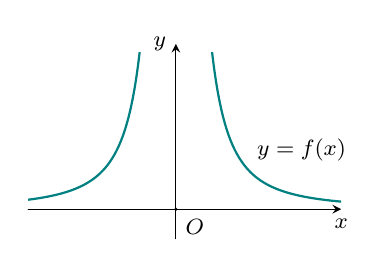
\begin{tikzpicture}[scale=.75, font=\footnotesize, line join=round, line cap=round,>=stealth]
			\def\xmin{-2.5} \def\xmax{2.8}
			\def\ymin{-0.5} \def\ymax{2.8}
			%\draw[color=gray!50,dashed] (\xmin,\ymin) grid (\xmax,\ymax);
			\draw[->] (\xmin,0)--(0,0)node [below right]{$O$}-- (\xmax,0) node [below]{$x$};
			\draw[->] (0,\ymin)--(0,\ymax) node [left]{$y$};
			\begin{scope}
				\clip (\xmin,\ymin) rectangle (\xmax,\ymax-.15);
				\draw[samples=200,smooth,variable=\x,thick, teal] plot[domain=\xmin:-0.5] (\x,{1/(\x)^2});
				\draw[samples=200,smooth,variable=\x,thick, teal] plot[domain=0.5:\xmax] (\x,{1/(\x)^2});
			\end{scope}
			\draw[ thick] (1.2,1)node[right]{$y=f(x)$};
			\foreach \x/\y in{0/0} \fill(\x,\y)circle(.03);
		\end{tikzpicture}	
	}
	% \dapso{Hàm số đã cho liên tục trên các khoảng $(-\infty;0)$ và $(0;+\infty)$. Gián đoạn tại điểm $x=0$.}
	\loigiai{
		Vì hàm số đã cho có tập xác định $\mathscr{D}=\mathbb{R}\setminus \{0\}$ nên
		\begin{itemize}
			\item $f(x)$ xác định trên khoảng $(-\infty;0)$ nên liên tục trên khoảng này.
			\item $f(x)$ xác định trên khoảng $(0;+\infty)$ nên liên tục trên khoảng này.
			\item $f(x)$ không xác định tại điểm $x=0$ nên gián đoạn tại điểm này.
		\end{itemize}	
	}
\end{vd}

% \subsubsection{Bài tập rèn luyện}
% % \centerline{\fcolorbox{teal}{yellow!50}{\bf {BÀI TẬP TỰ LUẬN }}}
% \begin{bt}%[DCHT Toán 11 - KNTT -Vũ Hồng Toàn]%[1K5YG-2]
% 	\immini{
% 		Cho hàm số $y=f(x)$ xác định trên $\mathscr{D}=\mathbb{R}$ và có đồ thị như hình vẽ bên.\\ Xét tính liên tục của hàm số $y=f(x)$ trên $\mathscr{D}$.	
% 	}
% 	{
% 		\begin{tikzpicture}[scale=.75, font=\footnotesize, line join=round, line cap=round,>=stealth]
% 			\def\a{1} \def\b{-2} \def\c{0} %\def\d{1} % Hệ số
% 			\def\xmin{-2} \def\xmax{2}
% 			\def\ymin{-1.5} \def\ymax{1.5}
% 			\draw[->] (\xmin,0)--(0,0)node [above right]{$O$}-- (\xmax,0) node [below]{$x$};
% 			\draw[->] (0,\ymin)--(0,\ymax) node [left]{$y$};
% 			\clip (\xmin+0.1,\ymin+0.1) rectangle (\xmax-0.1,\ymax-0.1);
% 			\draw[smooth,samples=100,thick ] plot(\x,{\a*(\x)^4+\b*(\x)^2+\c});
% 			\draw[ thick] (-.7,1)node[below]{$y=f(x)$};
% 		\end{tikzpicture}	
% 	}	
% 	% \dapso{Hàm số đã cho liên tục trên $\mathbb{R}$.}
% 	\loigiai{
% 		Do đồ thị hàm số là một đường liền nét trên $\mathscr{D}$ nên hàm số $y=f(x)$ liên tục trên $\mathscr{D}=\mathbb{R}$.}
% \end{bt}
% \begin{bt}%[DCHT Toán 11 - KNTT -Vũ Hồng Toàn]%[1K5BG-2]
% 	\immini{
% 		Cho hàm số $y=f(x)$ xác định trên $\mathscr{D}=\mathbb{R}$ và có đồ thị như hình vẽ bên. Xét tính liên tục của hàm số $y=f(x)$ trên $\mathscr{D}$.	
% 	}
% 	{
% 		\begin{tikzpicture}[scale=.75, font=\normalsize, line join=round, line cap=round,>=stealth]
% 			\def\a{2} %\def\b{-2} \def\c{0} %\def\d{1} % Hệ số
% 			\def\xmin{-2.5} \def\xmax{2.5}
% 			\def\ymin{-0.5} \def\ymax{3}
% 			%\draw[color=gray!50,dashed] (\xmin,\ymin) grid (\xmax,\ymax);
% 			\draw[->] (\xmin,0)--(0,0)node [below right]{$O$}-- (\xmax,0) node [below]{$x$};
% 			\draw[->] (0,\ymin)--(0,\ymax) node [left]{$y$};
% 			\clip (\xmin+0.1,\ymin+0.1) rectangle (\xmax-0.1,\ymax-0.1);
% 			\draw[smooth,samples=100,thick ] plot(\x,{\a^(\x)}) (.5,1) node [right]{$y=f(x)$};
% 		\end{tikzpicture}	
% 	}
% 	% \dapso{Hàm số đã cho liên tục trên $\mathbb{R}$.}
% 	\loigiai{
% 		Do đồ thị hàm số là một đường liền nét trên $\mathscr{D}$ nên hàm số $y=f(x)$ liên tục trên $\mathscr{D}=\mathbb{R}$.}
% \end{bt}
% \begin{bt}%[DCHT Toán 11 - KNTT -Vũ Hồng Toàn]%[1K5KG-2]
% 	\immini{
% 		Cho hàm số $y=f(x)$ xác định trên $\mathscr{D}=\mathbb{R}$ và có đồ thị như hình vẽ bên. Xét tính liên tục của hàm số $y=f(x)$ trên $\mathscr{D}$.	
% 	}
% 	{
% 		\begin{tikzpicture}[scale=1, font=\normalsize, line join=round, line cap=round,>=stealth]
% 			\def\xmin{-2} \def\xmax{3.5}
% 			\def\ymin{-.5} \def\ymax{2.5}
% 			\draw[->] (\xmin,0)--(0,0)node [below right]{$O$}-- (\xmax,0) node [below]{$x$};
% 			\draw[->] (0,\ymin)--(0,\ymax) node [left]{$y$};
% 			\clip (\xmin+0.1,\ymin+0.1) rectangle (\xmax-0.1,\ymax-0.1);
% 			\draw[smooth,samples=100,thick ] plot[domain=-1.5:1.5](\x,{(\x)^2})--(3,-.25) 
% 			(-1,1) node [left]{$y=f(x)$}; 
% 			\draw[dashed] (1.5,2.25)--(1.5,0) node [below]{$2$} ;
% 		\end{tikzpicture}	
% 	}
	
% 	% \dapso{Hàm số đã cho liên tục trên $\mathbb{R}$.}
% 	\loigiai{
% 		Do đồ thị hàm số là một đường liền nét trên $\mathscr{D}$ nên hàm số $y=f(x)$ liên tục trên $\mathscr{D}=\mathbb{R}$.}
% \end{bt}
% \begin{bt}%[DCHT Toán 11 - KNTT -Vũ Hồng Toàn]%[1K5KG-2]
% 	\immini{
% 		Cho hàm số $y=f(x)$ có đồ thị như hình vẽ bên.\\ Xét tính liên tục của hàm số $y=f(x)$ tại điểm $x_0=2$.	
% 	}
% 	{
% 		\begin{tikzpicture}[scale=1, font=\normalsize, line join=round, line cap=round,>=stealth]
% 			\def\xmin{-2} \def\xmax{3.5}
% 			\def\ymin{-.5} \def\ymax{2.5}
% 			\draw[->] (\xmin,0)--(0,0)node [below right]{$O$}-- (\xmax,0) node [below]{$x$};
% 			\draw[->] (0,\ymin)--(0,\ymax) node [left]{$y$};
% 			\clip (\xmin+0.1,\ymin+0.1) rectangle (\xmax-0.1,\ymax-0.1);
% 			\draw[smooth,samples=100,thick ] plot[domain=-1.5:1.5](\x,{(\x)^2}) (1.5,1.5)--(3,-.25) 
% 			(-1,1) node [left]{$y=f(x)$}; 
% 			\draw[dashed] (1.5,2.25)--(1.5,0) node [below]{$2$} (1.5,1.5)--(0,1.5)node [left]{$2$};
% 			\foreach \x/\y in{0/0,1.5/0,1.5/1.5,0/1.5,1.5/2.25} \fill(\x,\y)circle(.03);
% 		\end{tikzpicture}	
% 	}
% 	% \dapso{Hàm số đã cho gián đoạn tại $x_0=2$. }
% 	\loigiai{
% 		Ta có $\lim\limits_{x\to{2}^-}f(x)>2$ và $\lim\limits_{x\to{2}^+}f(x)=2$. Do đó $\lim\limits_{x\to{2}^-}f(x)\ne \lim\limits_{x\to{2}^+}f(x)$. Vậy hàm số đã cho gián đoạn tại $x_0=2$.
% 	}
% \end{bt}

% \begin{bt}%[DCHT Toán 11 - KNTT -Vũ Hồng Toàn]%[1K5KG-2]
% 	\immini{
% 		Cho hàm số $y=f(x)$ có đồ thị như hình vẽ bên.\\ Xét tính liên tục của hàm số $y=f(x)$ tại điểm $x_0=1$.	
% 	}
% 	{
% 		\begin{tikzpicture}[scale=.5, font=\footnotesize, line join=round, line cap=round,>=stealth]
% 			\def\a{0} \def\b{1} \def\c{1} \def\d{-1}
% 			\pgfmathsetmacro\tcd{int(round(-\d/\c))} \pgfmathsetmacro\tcn{int(round(\a/\c))} 
% 			\pgfmathsetmacro\xmin{\tcd-2.5} \pgfmathsetmacro\xmax{\tcd+2.5}
% 			\pgfmathsetmacro\ymin{\tcn-2.5} \pgfmathsetmacro\ymax{\tcn+2.5}
% 			\draw[->] (\xmin,0)--(0,0)node [below right]{$O$}-- (\xmax,0) node [below]{$x$};
% 			\draw[->] (0,\ymin)--(0,\ymax) node [left]{$y$};
% 			\draw[dash pattern=on 2pt off 1.5pt] (\tcd,\ymin)--(\tcd,\ymax) (\tcd,0)node [below right]{$\tcd$};
% 			\begin{scope}
% 				\clip (\xmin,\ymin) rectangle (\xmax-.1,\ymax-.1);
% 				\draw[samples=200,smooth,variable=\x,thick, teal] plot[domain=\xmin:\tcd-0.3] (\x,{(\a*(\x)+\b)/(\c*(\x)+\d)});
% 				\draw[samples=200,smooth,variable=\x,thick, teal] plot[domain=\tcd+.3:\xmax] (\x,{(\a*(\x)+\b)/(\c*(\x)+\d)});
% 			\end{scope}
% 			\draw[ thick] (1.2,-1.5)node[right]{$y=f(x)$};
% 			\foreach \x/\y in{0/0,1/0} \fill(\x,\y)circle(.03);
% 		\end{tikzpicture}	
% 	}
% 	% \dapso{Hàm số đã cho gián đoạn tại $x_0=1$. }
% 	\loigiai{
% 		Ta có $\lim\limits_{x\to{1}^-}f(x)=-\infty$ và $\lim\limits_{x\to{1}^+}f(x)=+\infty$. Do đó $\lim\limits_{x\to{1}^-}f(x)\ne \lim\limits_{x\to{1}^+}f(x)$.\\ Vậy hàm số đã cho gián đoạn tại $x_0=1$.
% 	}
% \end{bt}

\subsubsection{Câu hỏi trắc nghiệm}
\Opensolutionfile{ans}[ans/ans-1K5-3-Dang1]

\begin{ex}%[DCHT Toán 11 - KNTT -Vũ Hồng Toàn]%[1K5YG-2]
	\immini{
		Cho đồ thị hàm số $y=f(x)$ có đồ thị như hình vẽ bên. Chọn mệnh đề đúng trong các mệnh đề sau:
		\choice[1]
		{Hàm số $y=f(x)$ liên tục trên $\mathbb{R}$}
		{\True Hàm số $y=f(x)$ liên tục trên khoảng $(0,+\infty)$}
		{Hàm số $y=f(x)$ liên tục tại điểm $x_0=0$}
		{$\lim\limits_{x\to{0}^+}f(x)=+\infty$}	
	}
	{
		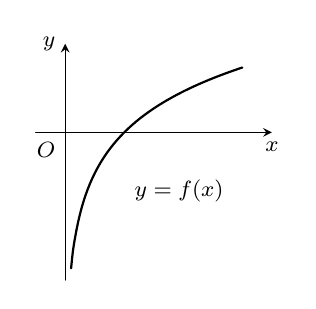
\begin{tikzpicture}[scale=.75, font=\footnotesize, line join=round, line cap=round,>=stealth]
			\def\xmin{-.5} \def\xmax{3.5}
			\def\ymin{-2.5} \def\ymax{1.5}
			\draw[->] (\xmin,0)--(0,0)node [below left]{$O$}-- (\xmax,0) node [below]{$x$};
			\draw[->] (0,\ymin)--(0,\ymax) node [left]{$y$};
			\clip (\xmin+0.1,\ymin+0.1) rectangle (\xmax-0.1,\ymax-0.1);
			\draw[smooth,samples=100,thick ] plot[domain=.1:3](\x,{ln(\x)}) 
			(1,-1) node [right]{$y=f(x)$}; 
		\end{tikzpicture}	
	}	
	\loigiai
	{
		Đồ thị hàm số là một đường liền nét trên khoảng $(0,+\infty)$ nên liên tục trên khoảng này.
	}
\end{ex}
%Cau2
\begin{ex}%[DCHT Toán 11 - KNTT -Vũ Hồng Toàn]%[1K5YG-2]
	\immini{
		Cho đồ thị hàm số $y=f(x)$ có đồ thị như hình vẽ bên. Chọn mệnh đề \textbf{sai} trong các mệnh đề sau:
		\choice[1]
		{\True $\lim\limits_{x\to{+\infty}}f(x)=-\infty$}
		{Hàm số $y=f(x)$ liên tục trên $\mathbb{R}$}
		{$\lim\limits_{x\to{+\infty}}f(x)=+\infty$}
		{$\lim\limits_{x\to{-\infty}}f(x)=-\infty$}	
	}
	{
		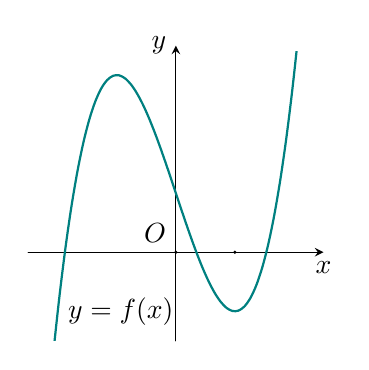
\begin{tikzpicture}[scale=.75, font=\normalsize, line join=round, line cap=round,>=stealth]
			\def\a{1} \def\b{0} \def\c{-3} \def\d{1}
			\def\f(#1){\a*(#1)^3+\b*(#1)^2+\c*(#1)+\d}
			\pgfmathsetmacro\tdx{int(round(-\b/(3*\a)))} \pgfmathsetmacro\tdy{int(round(\f(\tdx))}
			\pgfmathsetmacro\xmin{\tdx-2.5} \pgfmathsetmacro\xmax{\tdx+2.5}
			\pgfmathsetmacro\ymin{\tdy-2.5} \pgfmathsetmacro\ymax{\tdy+2.5}
			%\draw[color=gray!50,dashed] (\xmin,\ymin) grid (\xmax,\ymax);
			\draw[->] (\xmin,0)--(0,0)node [above left]{$O$}-- (\xmax,0) node [below]{$x$};
			\draw[->] (0,\ymin)--(0,\ymax) node [left]{$y$};
			\begin{scope}
				\clip (\xmin,\ymin) rectangle (\xmax-.1,\ymax-.1);
				\draw[samples=100,smooth,thick, teal] plot(\x,{\f(\x)});
			\end{scope}
			\draw[ thick] (-2,-1)node[right]{$y=f(x)$};
			\foreach \x/\y in{0/0,1/0} \fill(\x,\y)circle(.03);
		\end{tikzpicture} 	
	}
	\loigiai
	{
		Quan sát đồ thị hàm số, ta có
		\begin{itemize}
			\item Hàm số $y=f(x)$ liên tục trên $\mathbb{R}$.
			\item $\lim\limits_{x\to{+\infty}}f(x)=+\infty$.
			\item $\lim\limits_{x\to{-\infty}}f(x)=-\infty$.
		\end{itemize}
	}
\end{ex}
%Cau3
\begin{ex}%[DCHT Toán 11 - KNTT -Vũ Hồng Toàn]%[1K5YG-2]
	\immini{
		Cho đồ thị hàm số $y=f(x)$ có đồ thị như hình vẽ bên. Chọn mệnh đề đúng trong các mệnh đề sau:
		\choice
		{$\lim\limits_{x\to{+\infty}}f(x)=-\infty$}
		{\True Hàm số $y=f(x)$ liên tục trên khoảng $(0;+\infty)$}
		{Hàm số $y=f(x)$ liên tục tại điểm $x_0=0$}
		{Hàm số $y=f(x)$ liên tục trên $\mathbb{R}$}	
	}
	{
		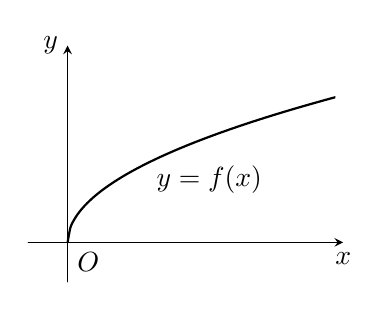
\begin{tikzpicture}[scale=1, font=\normalsize, line join=round, line cap=round,>=stealth]
			\def\xmin{-.5} \def\xmax{3.5}
			\def\ymin{-.5} \def\ymax{2.5}
			%\draw[color=gray!50,dashed] (\xmin,\ymin) grid (\xmax,\ymax);
			\draw[->] (\xmin,0)--(0,0)node [below right]{$O$}-- (\xmax,0) node [below]{$x$};
			\draw[->] (0,\ymin)--(0,\ymax) node [left]{$y$};
			\clip (\xmin+0.1,\ymin+0.1) rectangle (\xmax-0.1,\ymax-0.1);
			\draw[smooth,samples=100,thick ] plot[domain=0:3.5](\x,{sqrt(\x)}) 
			(1,.8) node [right]{$y=f(x)$}; 
		\end{tikzpicture}	
	}
	\loigiai
	{
		Quan sát đồ thị hàm số, thấy đồ thị hàm số là một đường liền nét trên khoảng $(0;+\infty)$ do đó hàm số đã cho liên tục trên khoảng này.
	}
\end{ex}
%Cau4
\begin{ex}%[DCHT Toán 11 - KNTT -Vũ Hồng Toàn]%[1K5YG-2]
	\immini{
		Cho đồ thị hàm số $y=f(x)$ có đồ thị như hình vẽ bên. Chọn mệnh đề \textbf{sai} trong các mệnh đề sau:
		\choice[1]
		{Hàm số gián đoạn tại điểm $x_0=0$}
		{Hàm số liên tục trên khoảng $(-\infty;0)$}
		{\True Hàm số $y=f(x)$ liên tục trên $\mathbb{R}$}
		{Hàm số liên tục trên khoảng $(0;+\infty)$}	
	}
	{
		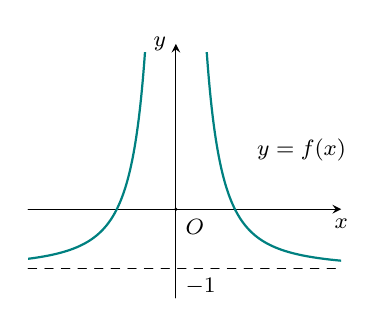
\begin{tikzpicture}[scale=.75, font=\footnotesize, line join=round, line cap=round,>=stealth]
			\def\xmin{-2.5} \def\xmax{2.8}
			\def\ymin{-1.5} \def\ymax{2.8}
			%\draw[color=gray!50,dashed] (\xmin,\ymin) grid (\xmax,\ymax);
			\draw[->] (\xmin,0)--(0,0)node [below right]{$O$}-- (\xmax,0) node [below]{$x$};
			\draw[->] (0,\ymin)--(0,\ymax) node [left]{$y$};
			\begin{scope}
				\clip (\xmin,\ymin) rectangle (\xmax,\ymax-.15);
				\draw[samples=200,smooth,variable=\x,thick, teal] plot[domain=\xmin:-0.5] (\x,{1/(\x)^2-1});
				\draw[samples=200,smooth,variable=\x,thick, teal] plot[domain=0.5:\xmax] (\x,{1/(\x)^2-1});
			\end{scope}
			\draw[dashed](\xmin,-1)--(\xmax,-1) (0,-1)node[below right]{$-1$};
			\draw[ thick] (1.2,1)node[right]{$y=f(x)$};
			\foreach \x/\y in{0/0} \fill(\x,\y)circle(.03);
		\end{tikzpicture}	
	}
	
	\loigiai
	{
		Quan sát đồ thị hàm số, ta có
		\begin{itemize}
			\item Hàm số gián đoạn tại điểm $x_0=0$.
			\item Hàm số liên tục trên khoảng $(-\infty;0)$.
			\item Hàm số liên tục trên khoảng $(0;+\infty)$.
		\end{itemize}
	}
\end{ex}
%Cau5
\begin{ex}%[DCHT Toán 11 - KNTT -Vũ Hồng Toàn]%[1K5BG-2]
	\immini{
		Cho đồ thị hàm số $y=f(x)$ có đồ thị như hình vẽ bên. Chọn mệnh đề \textbf{sai} trong các mệnh đề sau:
		\choice[1]
		{Hàm số gián đoạn tại điểm $x_0=1$}
		{Hàm số liên tục trên khoảng $(-\infty;1)$}
		{\True Hàm số $y=f(x)$ liên tục trên $\mathbb{R}$}
		{Hàm số liên tục trên khoảng $(1;+\infty)$}		
	}
	{
		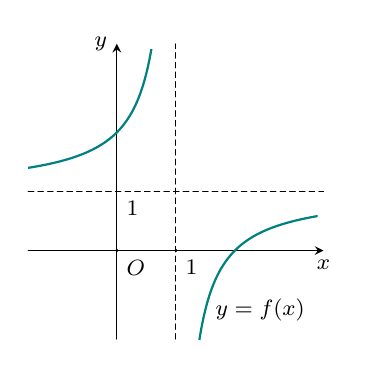
\begin{tikzpicture}[scale=.75, font=\footnotesize, line join=round, line cap=round,>=stealth]
			\def\a{1} \def\b{-2} \def\c{1} \def\d{-1}
			\pgfmathsetmacro\tcd{int(round(-\d/\c))} \pgfmathsetmacro\tcn{int(round(\a/\c))} 
			\pgfmathsetmacro\xmin{\tcd-2.5} \pgfmathsetmacro\xmax{\tcd+2.5}
			\pgfmathsetmacro\ymin{\tcn-2.5} \pgfmathsetmacro\ymax{\tcn+2.5}
			%\draw[color=gray!50,dashed] (\xmin,\ymin) grid (\xmax,\ymax);
			\draw[->] (\xmin,0)--(0,0)node [below right]{$O$}-- (\xmax,0) node [below]{$x$};
			\draw[->] (0,\ymin)--(0,\ymax) node [left]{$y$};
			\draw[dash pattern=on 2pt off 1.5pt] (\tcd,\ymin)--(\tcd,\ymax) (\tcd,0)node [below right]{$\tcd$}
			(\xmin,\tcn)--(\xmax,\tcn) (0,\tcn)node [below right]{$\tcn$};
			\begin{scope}
				\clip (\xmin,\ymin) rectangle (\xmax-.1,\ymax-.1);
				\draw[samples=200,smooth,variable=\x,thick, teal] plot[domain=\xmin:\tcd-0.3] (\x,{(\a*(\x)+\b)/(\c*(\x)+\d)});
				\draw[samples=200,smooth,variable=\x,thick, teal] plot[domain=\tcd+.3:\xmax] (\x,{(\a*(\x)+\b)/(\c*(\x)+\d)});
			\end{scope}
			\draw[ thick] (1.5,-1)node[right]{$y=f(x)$};
			\foreach \x/\y in{0/0,1/0} \fill(\x,\y)circle(.03);
		\end{tikzpicture}	
	}
	\loigiai
	{
		Quan sát đồ thị hàm số, ta có
		\begin{itemize}
			\item Hàm số gián đoạn tại điểm $x_0=1$.
			\item Hàm số liên tục trên khoảng $(-\infty;1)$.
			\item Hàm số liên tục trên khoảng $(1;+\infty)$.
		\end{itemize}
	}
\end{ex}
%Cau6
\begin{ex}%[DCHT Toán 11 - KNTT -Vũ Hồng Toàn]%[1K5BG-2]
	\immini{
		Cho đồ thị hàm số $y=f(x)$ có đồ thị như hình vẽ bên. Chọn mệnh đề đúng trong các mệnh đề sau:
		\choice[1]
		{Hàm số $y=f(x)$ liên tục trên $\mathbb{R}$}
		{$\lim\limits_{x\to{+\infty}}f(x)=-\infty$}
		{Hàm số liên tục tại điểm $x_0=-2$}
		{\True Hàm số gián đoạn tại điểm $x_0=-2$}	
	}
	{
		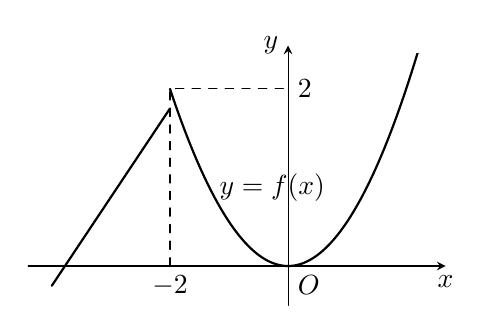
\begin{tikzpicture}[scale=1, font=\normalsize, line join=round, line cap=round,>=stealth]
			\def\xmin{-3.3} \def\xmax{2}
			\def\ymin{-.5} \def\ymax{2.8}
			\draw[->] (\xmin,0)--(0,0)node [below right]{$O$}-- (\xmax,0) node [below]{$x$};
			\draw[->] (0,\ymin)--(0,\ymax) node [left]{$y$} ;
			\clip (\xmin+0.1,\ymin+0.1) rectangle (\xmax-0.1,\ymax-0.1);
			\draw[smooth,samples=100,thick ] plot[domain=-1.5:2](\x,{(\x)^2})  
			(-1,1) node [right]{$y=f(x)$}; 
			\draw[thick ] (-3,-.25)--(-1.5,2);
			\draw[dashed] (-1.5,0)node [below]{$-2$}|-(0,2.25) node [right]{$2$} ;
		\end{tikzpicture}	
	} 
	
	\loigiai
	{
		Quan sát đồ thị hàm số, ta có	
		\begin{itemize}
			\item Đồ thị hàm số là các đường liền nét trên các khoảng $(-\infty;-2)$, $(-2;+\infty)$ do đó hàm số liên tục trên các khoảng này.
			\item $\lim\limits_{x\to{+\infty}}f(x)=+\infty$
			\item Ta có $\lim\limits_{x\to{(-2)}^-}f(x)<f(-2)=2$ và $\lim\limits_{x\to{(-2)}^+}f(x)=f(-2)=2$. Do đó $\lim\limits_{x\to{(-2)}^-}f(x)\ne \lim\limits_{x\to{(-2)}^+}f(x)$.\\
			Vậy hàm số đã cho gián đoạn tại $x_0=-2$.
		\end{itemize}
	}
\end{ex}
%Cau7
\begin{ex}%[DCHT Toán 11 - KNTT -Vũ Hồng Toàn]%[1K5BG-2]
	\immini{
		Cho đồ thị hàm số $y=f(x)$ có đồ thị như hình vẽ bên. Chọn mệnh đề đúng trong các mệnh đề sau:
		\choice[1]
		{\True $\lim\limits_{x\to{1}^+}f(x)=+\infty$}
		{Hàm số $y=f(x)$ liên tục trên $\mathbb{R}$}
		{$\lim\limits_{x\to{1}^+}f(x)=-\infty$}
		{$\lim\limits_{x\to{1}^-}f(x)=+\infty$}	
	}
	{
		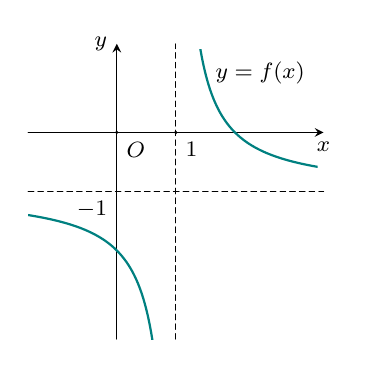
\begin{tikzpicture}[scale=.75, font=\footnotesize, line join=round, line cap=round,>=stealth]
			\def\a{-1} \def\b{2} \def\c{1} \def\d{-1}
			\pgfmathsetmacro\tcd{int(round(-\d/\c))} \pgfmathsetmacro\tcn{int(round(\a/\c))} 
			\pgfmathsetmacro\xmin{\tcd-2.5} \pgfmathsetmacro\xmax{\tcd+2.5}
			\pgfmathsetmacro\ymin{\tcn-2.5} \pgfmathsetmacro\ymax{\tcn+2.5}
			%\draw[color=gray!50,dashed] (\xmin,\ymin) grid (\xmax,\ymax);
			\draw[->] (\xmin,0)--(0,0)node [below right]{$O$}-- (\xmax,0) node [below]{$x$};
			\draw[->] (0,\ymin)--(0,\ymax) node [left]{$y$};
			\draw[dash pattern=on 2pt off 1.5pt] (\tcd,\ymin)--(\tcd,\ymax) (\tcd,0)node [below right]{$\tcd$}
			(\xmin,\tcn)--(\xmax,\tcn) (0,\tcn)node [below left]{$\tcn$};
			\begin{scope}
				\clip (\xmin,\ymin) rectangle (\xmax-.1,\ymax-.1);
				\draw[samples=200,smooth,variable=\x,thick, teal] plot[domain=\xmin:\tcd-0.3] (\x,{(\a*(\x)+\b)/(\c*(\x)+\d)});
				\draw[samples=200,smooth,variable=\x,thick, teal] plot[domain=\tcd+.3:\xmax] (\x,{(\a*(\x)+\b)/(\c*(\x)+\d)});
			\end{scope}
			\draw[ thick] (1.5,1)node[right]{$y=f(x)$};
			\foreach \x/\y in{0/0,1/0} \fill(\x,\y)circle(.03);
		\end{tikzpicture}	
	}
	
	\loigiai
	{
		Quan sát đồ thị hàm số, ta có	
		\begin{itemize}
			\item Đồ thị hàm số là các đường liền nét trên các khoảng $(-\infty;1)$, $(1;+\infty)$ do đó hàm số liên tục trên các khoảng này.
			\item $\lim\limits_{x\to{+\infty}}f(x)=-1$.
			\item Ta có $\lim\limits_{x\to{1}^-}f(x)=-\infty$ và $\lim\limits_{x\to{1}^+}f(x)=+\infty$. Do đó $\lim\limits_{x\to{1}^-}f(x)\ne \lim\limits_{x\to{1}^+}f(x)$.\\
			Vậy hàm số đã cho gián đoạn tại $x_0=1$.
		\end{itemize}
	}
\end{ex}
%Cau8
\begin{ex}%[DCHT Toán 11 - KNTT -Vũ Hồng Toàn]%[1K5KG-2]
	\immini{
		Cho đồ thị hàm số $y=f(x)$ có đồ thị như hình vẽ bên. Chọn mệnh đề đúng trong các mệnh đề sau:
		\choice[1]
		{Hàm số $y=f(x)$ gián đoạn tại $x_0=0$}
		{$\lim\limits_{x\to{+\infty}}f(x)=-1$}
		{$\lim\limits_{x\to{-\infty}}f(x)=-1$}
		{\True Hàm số $y=f(x)$ liên tục trên $\mathbb{R}$}	
	}
	{
		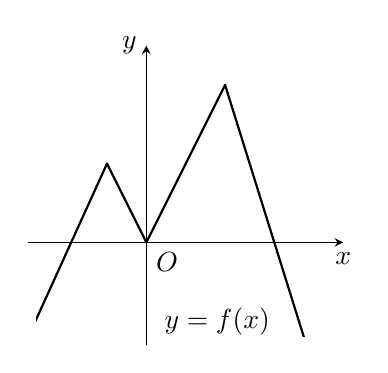
\begin{tikzpicture}[scale=1, font=\normalsize, line join=round, line cap=round,>=stealth]
			%	\def\a{2} %\def\b{-2} \def\c{0} %\def\d{1} % Hệ số
			\def\xmin{-1.5} \def\xmax{2.5}
			\def\ymin{-1.3} \def\ymax{2.5}
			%\draw[color=gray!50,dashed] (\xmin,\ymin) grid (\xmax,\ymax);
			\draw[->] (\xmin,0)--(0,0)node [below right]{$O$}-- (\xmax,0) node [below]{$x$};
			\draw[->] (0,\ymin)--(0,\ymax) node [left]{$y$};
			\clip (\xmin+0.1,\ymin+0.1) rectangle (\xmax-0.1,\ymax-0.1);
			\draw[thick ] (-1.5,-1.2)--(-.5,1)--(0,0)--(1,2)--(2,-1.2) 
			(1.7,-1) node [left]{$y=f(x)$}; 
		\end{tikzpicture}	
	}
	
	\loigiai
	{
		Quan sát đồ thị hàm số, ta có	
		\begin{itemize}
			\item Đồ thị hàm số là các đường liền nét trên khoảng $(-\infty;+\infty)$ do đó hàm số liên tục trên $\mathbb{R}$.
			\item $\lim\limits_{x\to{+\infty}}f(x)=-\infty$.
			\item $\lim\limits_{x\to{-\infty}}f(x)=-\infty$.
		\end{itemize}
	}
\end{ex}
%Cau9
\begin{ex}%[DCHT Toán 11 - KNTT -Vũ Hồng Toàn]%[1K5KG-2]
	\immini{
		Cho đồ thị hàm số $y=f(x)$ có đồ thị như hình vẽ bên. Chọn mệnh đề đúng trong các mệnh đề sau:
		\choice[1]
		{Hàm số $y=f(x)$ liên tục trên $\mathbb{R}$}
		{Hàm số $y=f(x)$ liên tục tại $x_0=-3$}
		{$\lim\limits_{x\to{-\infty}}f(x)=-\infty$}
		{\True Hàm số $y=f(x)$ gián đoạn tại $x_0=3$}	
	}
	{
		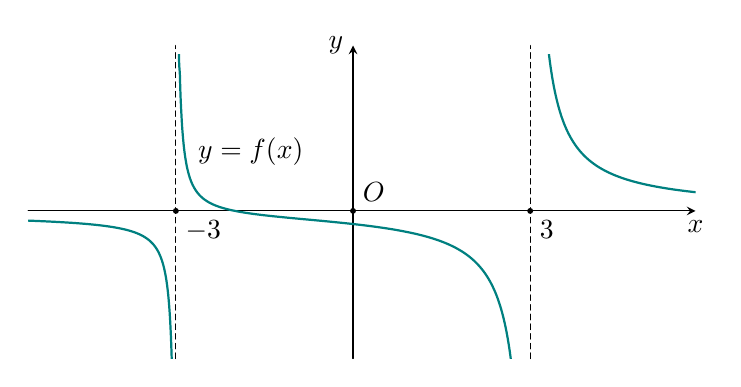
\begin{tikzpicture}[scale=.75, font=\normalsize, line join=round, line cap=round,>=stealth]
			\def\xmin{-5.5} \def\xmax{5.8}
			\def\ymin{-2.5} \def\ymax{2.8}
			%\draw[color=gray!50,dashed] (\xmin,\ymin) grid (\xmax,\ymax);
			\draw[->] (\xmin,0)--(0,0)node [above right]{$O$}-- (\xmax,0) node [below]{$x$};
			\draw[->] (0,\ymin)--(0,\ymax) node [left]{$y$};
			\draw[dash pattern=on 2pt off 1.5pt] (-3,\ymin)--(-3,\ymax) (3,\ymin)--(3,\ymax)
			(-3,0)node [below right]{$-3$} (3,0)node [below right]{$3$}
			;
			\begin{scope}
				\clip (\xmin,\ymin) rectangle (\xmax,\ymax-.15);
				\draw[samples=200,smooth,variable=\x,thick, teal] plot[domain=\xmin:-3.01] (\x,{(\x+2)/((\x)^2-9)});
				\draw[samples=200,smooth,variable=\x,thick, teal] plot[domain=-2.99:2.99] (\x,{(\x+2)/((\x)^2-9)});
				\draw[samples=200,smooth,variable=\x,thick, teal] plot[domain=3.01:\xmax] (\x,{(\x+2)/((\x)^2-9)});
			\end{scope}
			\draw[ thick] (-2.8,1)node[right]{$y=f(x)$};
			\foreach \x/\y in{0/0,-3/0,3/0} \fill(\x,\y)circle(.05);
		\end{tikzpicture} 	
	}
	\loigiai
	{
		Quan sát đồ thị hàm số, ta có	
		\begin{itemize}
			\item Đồ thị hàm số là các đường liền nét trên khoảng $(-\infty;-3)$, $(-3;3)$, $(3;+\infty) $ do đó hàm số liên tục trên các khoảng này.
			\item $\lim\limits_{x\to{-\infty}}f(x)=0$.
			\item Hàm số $y=f(x)$ gián đoạn tại các điểm $x_0=3$ và $x_0=-3$.
		\end{itemize}
	}
\end{ex}
%Cau10
\begin{ex}%[DCHT Toán 11 - KNTT -Vũ Hồng Toàn]%[1K5GG-2]
	\immini{
		Cho đồ thị hàm số $y=f(x)$ có đồ thị như hình vẽ bên. Chọn mệnh đề đúng trong các mệnh đề sau:
		\choice[1]
		{Hàm số $y=f(x)$ liên tục trên $\mathbb{R}$}
		{Hàm số $y=f(x)$ liên tục tại điểm $x_0=\dfrac{\pi}{2}$}
		{Hàm số $y=f(x)$ liên tục tại điểm $x_0=-\dfrac{\pi}{2}$}
		{\True Hàm số $y=f(x)$ gián đoạn tại điểm $x_0=\dfrac{\pi}{2}$}
	}
	{
		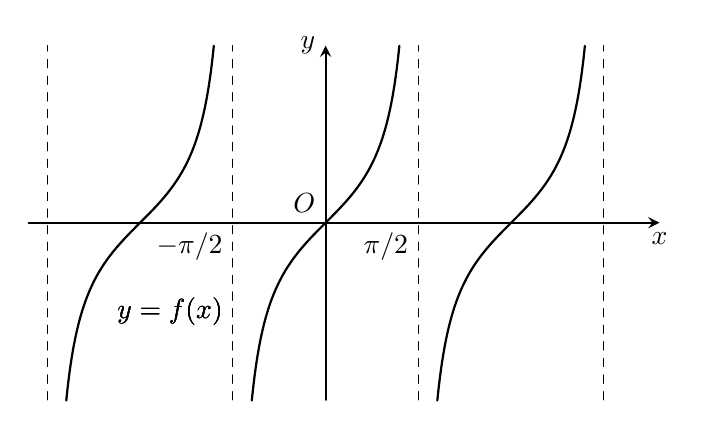
\begin{tikzpicture}[line join=round, line cap=round,thick,>=stealth,scale=.75 ]
			\draw[->](-1.6*pi,0)--(1.8*pi,0) node[below]{$x$};
			\draw[->](0,-3)--(0,3) node[left]{$y$};
			\draw (0,0) node[above left]{$O$};
			\foreach \i in {-1,0,1}{
				\pgfmathsetmacro{\start}{\i*pi-1.25}
				\pgfmathsetmacro{\left}{(\i-0.5)*pi}
				\pgfmathsetmacro{\end}{\i*pi+1.25}
				\draw[dashed, thin](\left,-3)--(\left,3);
				\draw[domain=\start:\end,samples=100,smooth ] plot(\x,{tan(\x r)}) (-3.7,-1.5) node[right]{$y=f(x)$};
			}
			\draw[dashed,thin] (1.5*pi,-3)--(1.5*pi,3);
			\draw (-pi/2,0) node [below left]{$-\pi/2$} (pi/2,0) node [below left]{$\pi/2$};
		\end{tikzpicture}	
	}
	\loigiai
	{
		Quan sát đồ thị hàm số, ta có	
		\begin{itemize}
			\item Đồ thị hàm số là các đường liền nét trên khoảng $(-\dfrac{\pi}{2};0)$, $(0;\dfrac{\pi}{2}) $ do đó hàm số liên tục trên các khoảng này.
			\item Hàm số $y=f(x)$ gián đoạn tại các điểm $x_0=\dfrac{\pi}{2}$ và $x_0=-\dfrac{\pi}{2}$.
		\end{itemize}
	}
\end{ex}
\Closesolutionfile{ans}
% \begin{indapan}{10}
% 	{ans/ans-1K5-3-Dang1}
% \end{indapan}

\begin{dang}{Hàm số liên tục tại một điểm}
	Để kiểm tra tính liên tục của hàm số $y=f(x)$ tại điểm $x=x_0$ ta cần làm như sau:
	\begin{itemize}
		\item Bước 1: Tính $\lim \limits_{x \to x_0} f(x)$.
		\item Bước 2: Tính $f(x_0)$.
		Nếu $\lim \limits_{x \to x_0} f(x) = f(x_0)$ thì kết luận hàm số $f(x)$ liên tục tại $x=x_0$.
		Nếu $\lim \limits_{x \to x_0} f(x) \ne f(x_0)$ thì kết luận hàm số $f(x)$ liên tục tại $x=x_0$.
	\end{itemize}
\end{dang}
\subsubsection{Ví dụ mẫu}
\begin{vd}%[DCHT Toán 11 - KNTT -Hứa Chí Ninh]%[1K5BG-3]
	Xét tính liên tục của hàm số $f(x)=\heva{&\dfrac{x^2-3x+2}{x-2}&\text{khi }x\neq 2\\&4x-7&\text{khi }x=2}$ tại điểm $x_0=2$.
	\loigiai{
		Ta có $f(x_0)=f(2)=4\cdot 2-7=1$.\\
		$\lim\limits_{x\rightarrow2}f(x)=\lim\limits_{x\rightarrow2}\dfrac{x^2-3x+2}{x-2}=\lim\limits_{x\rightarrow2}\dfrac{(x-1)(x-2)}{x-2}=\lim\limits_{x\rightarrow2}(x-1)=1$.\\
		Suy ra $f(2)=\lim\limits_{x\rightarrow 2}f(x)$ nên hàm số $f(x)$ liên tục tại điểm $x_0=2$.
	}
\end{vd}

\begin{vd}%[DCHT Toán 11 - KNTT -Hứa Chí Ninh]%[1K5BG-3]
	Xét tính liên tục của hàm số $f(x)=\begin{cases}
		\dfrac{1-\sqrt{2x-3}}{2-x}&\text{ nếu }\:x\ne2\\
		1&\text{ nếu }\:x=2
	\end{cases}$
	tại điểm $x_0=2$.
	\loigiai{Ta có
		\begin{itemize}
			\item $f(2)=1$.
			\item $\lim\limits_{x\to 2}f(x)=\lim\limits_{x\to 2}\dfrac{1-\sqrt{2x-3}}{2-x}=\lim\limits_{x\to 2}\dfrac{1-(2x-3)}{(2-x)(1+\sqrt{2x-3})}=\lim\limits_{x\to 2}\dfrac{2(2-x)}{(2-x)(1+\sqrt{2x-3})}\\
			=\lim\limits_{x\to 2}\dfrac{2}{1+\sqrt{2x-3}}=1=f(2)$
		\end{itemize}
		Vậy hàm số $f(x)$ liên tục tại $x_0=2$.}
\end{vd}

\begin{vd}%[DCHT Toán 11 - KNTT -Hứa Chí Ninh]%[1K5BG-3]
	Biết rằng $\lim\limits_{x\to 0} \dfrac{\sin x}{x}=1$. Hàm số $f\left( x \right)=\heva{&\dfrac{\tan x}{x} & \text{ khi }x\ne 0 \\&0 & \text{ khi }x=0}$. Xét tính liên tục của $y=f(x)$ tại $x=0$?
	 % \dapso{ $f\left( x \right)$ không liên tục tại $x=0$.}
	\loigiai{	Tập xác định $\mathscr{D}=\mathbb{R}\setminus \left\{ \dfrac{\pi }{2}+k\pi |k\in \mathbb{Z} \right\}$.\\
		Ta có $\lim\limits_{x\to 0} f\left( x \right)=\lim\limits_{x\to 0} \dfrac{\tan x}{x}=\lim\limits_{x\to 0} \dfrac{\sin x}{x}\cdot\dfrac{1}{\cos x}=1\cdot\dfrac{1}{\cos 0}=1\ne f\left( 0 \right)\Rightarrow $ $f\left( x \right)$ không liên tục tại $x=0$.}
\end{vd}
\begin{vd}%[DCHT Toán 11 - KNTT -Hứa Chí Ninh]%[1K5BG-3]
	Hàm số $f\left( x \right)=\left\{ \begin{array}{*{35}{l}}
		3 & \text{khi}\,\,x=-1 \\
		\dfrac{x^4+x}{x^2+x} & \text{khi}\,\,x\ne -1,\,\,x\ne 0 \\
		1 & \text{khi}\,\,x=0 \\
	\end{array} \right.$. Xét tính liên tục của hàm số tại $x=-1, x=0.$
	% \dapso{Hàm số liên tục tại $x=-1, x=0.$}
	\loigiai{
		Hàm số $y=f\left( x \right)$ có tập xác định $\mathscr{D}=\mathbb{R}$.\\
		Dễ thấy hàm số $y=f\left( x \right)$ liên tục trên mỗi khoảng $\left( -\infty ;-1 \right),\left( -1;0 \right)$ và $\left( 0;+\infty \right)$.\\
		(i) Xét tại $x=-1$, ta có\\
		$\lim\limits_{x\to -1} f\left( x \right)=\lim\limits_{x\to -1} \dfrac{x^4+x}{x^2+x}=\lim\limits_{x\to -1} \dfrac{x\left( x+1 \right)\left( {x^2}-x+1 \right)}{x\left( x+1 \right)}=\lim\limits_{x\to -1} \left( {x^2}-x+1 \right)=3=f\left( -1 \right).$ Vậy hàm số $y=f\left( x \right)$ liên tục tại $x=-1$.\\
		(ii) Xét tại $x=0$, ta có\\
		$\lim\limits_{x\to 0} f\left( x \right)=\lim\limits_{x\to 0} \dfrac{x^4+x}{x^2+x}=\lim\limits_{x\to 0} \dfrac{x\left( x+1 \right)\left( {x^2}-x+1 \right)}{x\left( x+1 \right)}=\lim\limits_{x\to 0} \left( {x^2}-x+1 \right)=1=f\left( 0 \right).$ Vậy hàm số $y=f\left( x \right)$ liên tục tại $x=0$.
	}
\end{vd}

\begin{vd}%[DCHT Toán 11 - KNTT -Hứa Chí Ninh]%[1K5BG-3]
	Xét tính liên tục của hàm số $f(x)=\begin{cases}
		x^2+1&\text{ nếu }\:x>0\\
		x&\text{ nếu }\:x\leq0
	\end{cases}$ tại điểm $x_0=0$.
	\loigiai{Ta có:
		\begin{itemize}
			\item $f(0)=0$.
			\item $\lim\limits_{x\to0^{+}}f(x)=\lim\limits_{x\to0^{+}}(x^2+1)=1$.
			\item $\lim\limits_{x\to0^{-}}f(x)=\lim\limits_{x\to0^{-}}x=0$.
		\end{itemize}
		Ta có: $f(0)=\lim\limits_{x\to0^{-}}f(x)\ne\lim\limits_{x\to0^{+}}f(x)$. Vậy hàm số $f(x)$ gián đoạn tại điểm $x=0$.
	}
\end{vd}

\begin{vd}%[DCHT Toán 11 - KNTT -Hứa Chí Ninh]%[1K5BG-3]
	Xét tính liên tục của hàm số $f\left( x \right)=\left\{ \begin{array}{*{35}{l}}
		1-\cos x & \text{khi }x\le 0 \\
		\sqrt{x+1} & \text{khi }x>0 \\
	\end{array} \right.$ tại $x=0?$
	% \dapso{Hàm số $y=f\left( x \right)$ gián đoạn tại $x=0$.}
	\loigiai{
		Hàm số xác định với mọi $x\in \mathbb{R}$.\\
		Ta có $f\left( x \right)$ liên tục trên $\left( -\infty ;0 \right)$ và $\left( 0;+\infty \right).$\\
		Mặt khác $\left\{ \begin{aligned}
			& f\left( 0 \right)=1 \\
			& \lim\limits_{x\to {0^{-}}} f\left( x \right)=\lim\limits_{x\to {0^{-}}} \left( 1-\cos x \right)=1-\cos 0=0 \\
			& \lim\limits_{x\to {0^{+}}} f\left( x \right)=\lim\limits_{x\to {0^{+}}} \sqrt{x+1}=\sqrt{0+1}=1 \\
		\end{aligned} \right.\Rightarrow f\left( x \right)$ gián đoạn tại $x=0$.
	}
\end{vd}

\subsubsection{Bài tập rèn luyện}
% \centerline{\fcolorbox{red}{yellow!50}{\bf {BÀI TẬP TỰ LUẬN}}}
\begin{bt}%[DCHT Toán 11 - KNTT -Hứa Chí Ninh]%[1K5BG-3]
	Xét tính liên tục của hàm số $f(x)=\begin{cases}
		\dfrac{x^2-6x+5}{x^2-1}&\text{ nếu }\: x\ne 1\\
		-2&\text{ nếu }\: x=1
	\end{cases}$ tại điểm $x_0=1$.
	\loigiai{Ta có: $f(1)=-2$.\\
		$\lim\limits_{x\to1}f(x)=\lim\limits_{x\to1}\dfrac{x^2-6x+5}{x^2-1}=\lim\limits_{x\to1}\dfrac{(x-5)(x-1)}{(x-1)(x+1)}=\lim\limits_{x\to1}\dfrac{x-5}{x+1}=-2=f(1)$.\\
		Vậy hàm số $f(x)$ liên tục tại $x=1$.}
\end{bt}
\begin{bt}%[DCHT Toán 11 - KNTT -Hứa Chí Ninh]%[1K5BG-3]
	Xét tính liên tục của hàm số $f(x)=\begin{cases}
		\dfrac{\sqrt{x}-2}{\sqrt{x+5}-3}&\text{ nếu }\:x\ne4\\
		-\dfrac{3}{2}&\text{ nếu }\:x=4
	\end{cases}$ tại điểm $x_0=4$.
	\loigiai{
		Ta có:
		\begin{itemize}
			\item $f(4)=-\dfrac{3}{2}$.
			\item $\lim\limits_{x\to 4}f(x)=\lim\limits_{x\to 4}\dfrac{\sqrt{x}-2}{\sqrt{x+5}-3}=\lim\limits_{x\to 4}\dfrac{(\sqrt{x+5}+3)(x-4)}{(x+5-9)(\sqrt{x}+2)}$\\
			$=\lim\limits_{x\to 4}\dfrac{\sqrt{x+5}+3}{\sqrt{x}+2}=\dfrac{6}{4}=\dfrac{3}{2}\ne f(4)$. 
		\end{itemize}
		Vậy hàm số $f(x)$ gián đoạn tại điểm $x=4$.
	}
\end{bt}

\begin{bt}%[DCHT Toán 11 - KNTT -Hứa Chí Ninh]%[1K5BG-3]
	Cho hàm số $f\left( x \right)=\left\{ \begin{aligned}
		& \dfrac{x^2}{x}\text{ khi }x<1,x\ne 0 \\
		& 0\text{ khi }x=0 \\
		& \sqrt{x}\text{ khi }x\ge 1 \\
	\end{aligned} \right..$ Xét tính liên tục của hàm số $f\left( x \right)$ tại $x=0, x=1?$
	% \dapso{Hàm số $y=f\left( x \right)$ liên tục tại $x=0$ và $x=1$.}
	\loigiai{
		Hàm số $y=f\left( x \right)$ có tập xác định $\mathscr{D}=\mathbb{R}$.\\
		Dễ thấy hàm số $y=f\left( x \right)$ liên tục trên mỗi khoảng $\left( -\infty ;0 \right),\left( 0;1 \right)$ và $\left( 1;+\infty \right)$.\\
		Ta có $\left\{ \begin{aligned}
			& f\left( 0 \right)=0 \\
			& \lim\limits_{x\to {0^{-}}} f\left( x \right)=\lim\limits_{x\to {0^{-}}} \dfrac{x^2}{x}=\lim\limits_{x\to {0^{-}}} x=0 \\
			& \lim\limits_{x\to {0^{+}}} f\left( x \right)=\lim\limits_{x\to {0^{+}}} \dfrac{x^2}{x}=\lim\limits_{x\to {0^{+}}} x=0 \\
		\end{aligned} \right.\Rightarrow f\left( x \right)$ liên tục tại $x=0.$\\
		Ta có $\left\{ \begin{aligned}
			& f\left( 1 \right)=1 \\
			& \lim\limits_{x\to {1^{-}}} f\left( x \right)=\lim\limits_{x\to {1^{-}}} \dfrac{x^2}{x}=\lim\limits_{x\to {1^{-}}} x=1 \\
			& \lim\limits_{x\to {1^{+}}} f\left( x \right)=\lim\limits_{x\to {1^{+}}} \sqrt{x}=1 \\
		\end{aligned} \right.\Rightarrow f\left( x \right)$ liên tục tại $x=1.$
	}
\end{bt}

\begin{bt}%[DCHT Toán 11 - KNTT -Hứa Chí Ninh]%[1K5BG-3]
	Cho hàm số $y=\left\{ \begin{aligned}
		& \dfrac{1-x^3}{1-x},\text{khi  }x<1 \\
		& 1\text{  },\text{khi  }x\ge 1 \\
	\end{aligned} \right.$. Xét tính liên tục phải của hàm số tại $x=1$?
	% \dapso{Hàm số liên tục phải tại $x=1.$}
	\loigiai{
		Ta có   $y\left( 1 \right)=1$.\\
		Ta có   $\lim\limits_{x\to {1^{+}}} y=1$; $\lim\limits_{x\to {1^{-}}} y=\lim\limits_{x\to {1^{-}}} \dfrac{1-x^3}{1-x}=\lim\limits_{x\to {1^{-}}} \dfrac{\left( 1-x \right)\left( 1+x+x^2 \right)}{1-x}=\lim\limits_{x\to {1^{-}}} \left( 1+x+x^2 \right)=4$.\\
		Nhận thấy $\lim\limits_{x\to {1^{+}}} y=y\left( 1 \right)$, suy ra $y$ liên tục phải tại $x=1$.}
\end{bt}
\begin{bt}%[DCHT Toán 11 - KNTT -Hứa Chí Ninh]%[1K5BG-3]
	
	Cho hàm số $y=\left\{ \begin{aligned}
		& \dfrac{x^2-7x+12}{x-3} & \text{ khi } x\ne 3 \\
		& -1 &\text{ khi }x=3 \\
	\end{aligned} \right.$. Xét tính liên tục của hàm số tại $x=3$.
	% \dapso{Hàm số đã cho có đạo hàm tại $x=3$}
	\loigiai{
		$\lim\limits_{x\to 3} \dfrac{x^2-7x+12}{x-3}=\lim\limits_{x\to 3} \left( x-4 \right)=-1=y\left( 3 \right)$ nên hàm số liên tục tại $x_0=3$.}
\end{bt}
\begin{bt}%[DCHT Toán 11 - KNTT -Hứa Chí Ninh]%[1K5KG-3]
	Cho hàm số $f\left( x \right)=\left\{ \begin{aligned}
		& \dfrac{x-2}{\sqrt{x+2}-2}&\text{ khi }x\ne 2 \\
		& 4&\text{ khi }x=2 \\
	\end{aligned} \right.$. Xét tính liên tục của hàm số tại $x=2$?
	% \dapso{Hàm số liên tục tại $x=2.$}
	\loigiai{
		Tập xác định  $\mathscr{D}=\mathbb{R}$.\\
		$\lim\limits_{x\to 2} f\left( x \right)=\lim\limits_{x\to 2} \dfrac{x-2}{\sqrt{x+2}-2}=\lim\limits_{x\to 2} \dfrac{\left( x-2 \right)\left( \sqrt{x+2}+2 \right)}{x-2}=\lim\limits_{x\to 2} \left( \sqrt{x+2}+2 \right)=4$.\\
		$f\left( 2 \right)=4$
		$\Rightarrow \lim\limits_{x\to 2} f\left( x \right)=f\left( 2 \right)$.
		Vậy hàm số liên tục tại $x=2$.}
\end{bt}
\begin{bt}%[DCHT Toán 11 - KNTT -Hứa Chí Ninh]%[1K5KG-3]% 
	Cho hàm số $f\left( x \right)=\left\{ \begin{aligned}
		& \dfrac{1-\cos x}{x^2}& \text{ khi } x\ne 0 \\
		& 1 &\text{ khi } x=0 \\
	\end{aligned} \right.\,\,$. Xét tính liên tục của hàm số tại $x=0?$
	% \dapso{Hàm số gián đoạn tại $x=0.$}
	\loigiai{
		Hàm số xác định trên $\mathbb{R}$.\\
		Ta có $f\left( 0 \right)=1$ và $\lim\limits_{x\to 0} f\left( x \right)=\lim\limits_{x\to 0} \dfrac{1-\cos x}{x^2}=\lim\limits_{x\to 0} \dfrac{2{\sin ^2}\dfrac{x}{2}}{4\cdot{{\left( \dfrac{x}{2} \right)}^2}}=\dfrac{1}{2}.$\\
		Vì $f\left( 0 \right)\ne \lim\limits_{x\to 0} f\left( x \right)$ nên $f\left( x \right)$ gián đoạn tại $x=0$. Do đó $f\left( x \right)$không có đạo hàm tại $x=0$.\\
		Vì $\forall x\ne 0$, $f\left( x \right)=\dfrac{1-\cos x}{x^2}\ge 0$ nên $f\left( \sqrt{2} \right)>0.$ Vậy $f\left( x \right)$ gián đoạn tại $x=0$.}
\end{bt}
\begin{bt}%[DCHT Toán 11 - KNTT -Hứa Chí Ninh]%[1K5BG-4]
	Cho hàm số $f\left( x \right)=\heva{& -x\cos x &\text{ khi } x<0 \\& \dfrac{x^2}{1+x}&\text{ khi } 0\le x<1 \\& {x^3}&\text{ khi } x\ge 1}$. Xét tính liên tục của hàm số tại $x=0?$
	% \dapso{Hàm số gián đoạn tại $x=1.$}
	\loigiai{
		$\bullet$ $f\left( x \right)$ liên tục tại $x\ne 0$ và $x\ne 1$.\\
		$\bullet$ Tại $x=0$\\
		$\lim\limits_{x\to {0^{-}}} f\left( x \right)=\lim\limits_{x\to {0^{-}}} \left( -x\cos x \right)=0$, $\lim\limits_{x\to {0^{+}}} f\left( x \right)=\lim\limits_{x\to {0^{+}}} \dfrac{x^2}{1+x}=0$, $f\left( 0 \right)=0$.\\
		Suy ra $\lim\limits_{x\to {0^{-}}} f\left( x \right)=\lim\limits_{x\to {0^{+}}} f\left( x \right)=f\left( 0 \right)$. Hàm số liên tục tại $x=0$.\\
		$\bullet$ Tại $x=1$\\
		$\lim\limits_{x\to {1^{-}}} f\left( x \right)=\lim\limits_{x\to {1^{-}}} \dfrac{x^2}{1+x}=\dfrac{1}{2}$, $\lim\limits_{x\to {1^{+}}} f\left( x \right)=\lim\limits_{x\to {1^{+}}} x^3=1$.\\
		Suy ra $\lim\limits_{x\to {1^{-}}} f\left( x \right)\ne \lim\limits_{x\to {1^{+}}} f\left( x \right)$. Hàm số gián đoạn tại $x=1$.}
\end{bt}
\subsubsection{Câu hỏi trắc nghiệm}
\Opensolutionfile{ans}[ans/ans-1K5-3-Dang2]
\begin{ex}%[DCHT Toán 11 - KNTT -Hứa Chí Ninh]%[1K5BG-1]
	Cho hàm số $y=f(x)$ xác định trên khoảng $K$ và $x_0\in K$. Hàm số $y=f(x)$ liên tục tại $x_0$ nếu
	\choice
	{$\lim \limits_{x\rightarrow x_0^+} f(x) = f(x_0)$}
	{$\lim \limits_{x\rightarrow x_0^-} f(x) = f(x_0)$ }
	{\True $\lim \limits_{x\rightarrow x_0} f(x)= f(x_0)$ }
	{$\lim \limits_{x\rightarrow x_0} f(x) \neq  f(x_0)$ }
	\loigiai{
		Theo định nghĩa: Cho hàm số $y=f(x)$ xác định trên khoảng $K$ và $x_0\in K$. Hàm số $y=f(x)$ liên tục tại $x_0$ nếu $\lim \limits_{x\rightarrow x_0} f(x)= f(x_0)$.
	}
\end{ex}

\begin{ex}%[DCHT Toán 11 - KNTT -Hứa Chí Ninh]%[1K5BG-3]
	Cho hàm số $f(x) = \dfrac{x^2 + 3x - 4}{x + 4}$ với $x \neq -4$. Để hàm số $f(x)$ liên tục tại $x = -4$ thì ta cần bổ sung giá trị $f(-4)$ bằng bao nhiêu?
	\choice
	{$5$}
	{\True $-5$}
	{$3$}
	{$0$}
	\loigiai{
		$f(-4) = \lim\limits_{x \to -4}\dfrac{x^2 + 3x - 4}{x + 4} = \lim\limits_{x \to -4}\dfrac{(x - 1)(x + 4)}{x + 4} = \lim\limits_{x \to -4}(x - 1) = -5$.
	}
\end{ex}
\begin{ex}%[DCHT Toán 11 - KNTT -Hứa Chí Ninh]%[1K5BG-3]	
	Cho hàm số $f\left( x \right)=\dfrac{2x-1}{x^3-x}$. Kết luận nào sau đây đúng?
	\choice
	{Hàm số liên tục tại $x=-1$}
	{Hàm số liên tục tại $x=0$}
	{Hàm số liên tục tại $x=1$}
	{\True Hàm số liên tục tại $x=\dfrac{1}{2}$}
	\loigiai{
		Tại $x=\dfrac{1}{2}$, ta có   $\lim\limits_{x\to \frac{1}{2}} f\left( x \right)=\lim\limits_{x\to \frac{1}{2}} \dfrac{2x-1}{x^3-1}=0=f\left( \dfrac{1}{2} \right)$. Vậy hàm số liên tục tại $x=2$.}
\end{ex}
\begin{ex}%[DCHT Toán 11 - KNTT -Hứa Chí Ninh]%[1K5BG-3]
	Hàm số nào sau đây liên tục tại $x=1$$\colon$ 
	\choice
	{$f\left( x \right)=\dfrac{x^2+x+1}{x-1}$}
	{$f\left( x \right)=\dfrac{x^2-x-2}{x^2-1}$}
	{\True $f\left( x \right)=\dfrac{x^2+x+1}{x}$}
	{$f\left( x \right)=\dfrac{x+1}{x-1}$}
	\loigiai{
		$\bullet$ $f\left( x \right)=\dfrac{x^2+x+1}{x-1}$\\
		$\lim\limits_{x\to {1^{+}}} f\left( x \right)=+\infty $ suy ra $f\left( x \right)$ không liên tục tại $x=1$.\\
		$\bullet$ $f\left( x \right)=\dfrac{x^2-x-2}{x^2-1}$\\
		$\lim\limits_{x\to {1^{+}}} f\left( x \right)=\lim\limits_{x\to {1^{+}}} \dfrac{x-2}{x-1}=-\infty $ suy ra $f\left( x \right)$ không liên tục tại $x=1$.\\
		$\bullet$ $f\left( x \right)=\dfrac{x^2+x+1}{x}$\\
		$\lim\limits_{x\to 1} f\left( x \right)=\lim\limits_{x\to 1} \dfrac{x^2+x+1}{x}=3=f\left( 1 \right)$ suy ra $f\left( x \right)$ liên tục tại $x=1$.\\
		$\bullet$ $f\left( x \right)=\dfrac{x+1}{x-1}$\\
		$\lim\limits_{x\to {1^{+}}} f\left( x \right)=\lim\limits_{x\to {1^{+}}} \dfrac{x+1}{x-1}=+\infty $ suy ra $f\left( x \right)$ không liên tục tại $x=1$.}
\end{ex}
\begin{ex}%[DCHT Toán 11 - KNTT -Hứa Chí Ninh]%[1K5BG-3]
	Hàm số nào dưới đây gián đoạn tại điểm $x_0=-1$.
	\choice
	{$y=\left( x+1 \right)\left( {x^2}+2 \right)$}
	{\True $y=\dfrac{2x-1}{x+1}$}
	{$y=\dfrac{x}{x-1}$}
	{$y=\dfrac{x+1}{x^2+1}$}
	\loigiai{
		Ta có $y=\dfrac{2x-1}{x+1}$ không xác định tại $x_0=-1$ nên gián đoạn tại $x_0=-1$.}
\end{ex}
\begin{ex}%[DCHT Toán 11 - KNTT -Hứa Chí Ninh]%[1K5BG-3]
	Hàm số nào sau đây gián đoạn tại $x=2$?
	\choice
	{\True $y=\dfrac{3x-4}{x-2}$}
	{$y=\sin x$}
	{$y=x^4-2x^2+1$}
	{$y=\tan x$}
	\loigiai{
		Ta có   $y=\dfrac{3x-4}{x-2}$ có tập xác định $\mathscr{D}=\mathbb{R}\setminus \left\{ 2 \right\}$, do đó gián đoạn tại $x=2$.}
\end{ex}
\begin{ex}%[DCHT Toán 11 - KNTT -Hứa Chí Ninh]%[1K5BG-3]
	Hàm số $y=\dfrac{x}{x+1}$ gián đoạn tại điểm $x_0$ bằng?
	\choice
	{ $x_0=2018$}
	{ $x_0=1$}
	{ $x_0=0$}
	{\True $x_0=-1$}
	\loigiai{
		Vì hàm số $y=\dfrac{x}{x+1}$ có tập xác định $\mathscr{D}=\mathbb{R}\setminus \left\{ -1 \right\}$ nên hàm số gián đoạn tại điểm $x_0=-1$.}
\end{ex}
\begin{ex}%[DCHT Toán 11 - KNTT -Hứa Chí Ninh]%[1K5BG-3]
	Hàm số nào dưới đây gián đoạn tại điểm $x=1$?
	\choice
	{$y=\dfrac{x-1}{x^2+x+1}$}
	{$y=\dfrac{x^2-x+1}{x+1}$}
	{$y=(x-1)(x^2+x+1)$}
	{\True $y=\dfrac{x^2+2}{x-1}$}
	\loigiai
	{
		Ta có $\lim\limits_{x\to1^+}\dfrac{x^2+2}{x-1}=+\infty$ và $\lim\limits_{x\to1^-}\dfrac{x^2+2}{x-1}=-\infty$ nên hàm số $y=\dfrac{x^2+2}{x-1}$ gián đoạn tại điểm $x=1$.
	}
\end{ex}
\begin{ex}%[DCHT Toán 11 - KNTT -Hứa Chí Ninh]%[1K5BG-3]
	Cho hàm số $y=\dfrac{x-3}{x^2-1}$. Mệnh đề nào sau đây đúng?
	\choice
	{\True Hàm số không liên tục tại các điểm $x=\pm 1$}
	{Hàm số liên tục tại mọi $x\in \mathbb{R}$}
	{Hàm số liên tục tại các điểm $x=-1$}
	{Hàm số liên tục tại các điểm $x=1$}
	\loigiai{
		Hàm số $y=\dfrac{x-3}{x^2-1}$ có tập xác định $\mathbb{R}\setminus \left\{ \pm 1 \right\}$. Do đó hàm số không liên tục tại các điểm $x=\pm 1$.}
\end{ex}
\begin{ex}%[DCHT Toán 11 - KNTT -Hứa Chí Ninh]%[1K5KG-3] 
	Cho hàm số $f(x)=\heva{&\dfrac{1-\cos x}{x^2}&\text{ khi } x\ne 0\\&1&\text{ khi } x=0}$.
	Khẳng định nào đúng trong các khẳng định sau?
	\choice
	{Hàm số gián đoạn tại $x=\sqrt{2}$}
	{$f(\sqrt{2})<0$}
	{$f(x)$ liên tục tại $x=0$}	
	{\True $f(x)$ gián đoạn tại $x=0$}
	\loigiai{
		Hàm số xác định trên $\mathbb{R}$.\\
		Ta có $f(0)=1$ và $\lim \limits_{x\to 0} f(x)=\lim \limits_{x\to 0} \dfrac{1-\cos x}{x^2}=\lim \limits_{x\to 0} \dfrac{2\sin ^2\dfrac{x}{2}}{4\cdot \left(\dfrac{x}{2}\right)^2}=\dfrac{1}{2}$.\\
		Vì $f(0)\ne \lim \limits_{x\to 0} f(x)$ nên $f(x)$ gián đoạn tại $x=0$.}
\end{ex}
\Closesolutionfile{ans}
% \begin{indapan}{10}
% 	{ans/ans-1K5-3-Dang2}
% \end{indapan}
\begin{dang}{Hàm số liên tục trên khoảng, đoạn}
	\begin{itemize}
		\item Hàm số $y=f(x)$ được gọi là liên tục trên một khoảng nếu nó liên tục tại mọi điểm của khoảng đó.
		\item Hàm số $y=f(x)$ được gọi là liên tục trên đoạn $[a,b]$ nếu nó liên tục trên khoảng $(a,b)$ và $$\mathop {\lim \limits{n \to +\infty}}\limits_{x \to {a^ + }} f\left( x \right) = f\left( a \right),{\rm{   }}\mathop {\lim \limits{n \to +\infty}}\limits_{x \to {b^ - }} f\left( x \right) = f\left( b \right).$$
		\item Đồ thị của hàm số liên tục trên một khoảng là một đường liền nét trên khoảng đó.
	\end{itemize}
\end{dang}
\subsubsection{Ví dụ mẫu}
\begin{vd}%[DCHT Toán 11 - KNTT -Hứa Chí Ninh]%[1K5KG-4]
	Xét tính liên tục của hàm số sau trên tập xác định của chúng.
	\begin{itemize}
		\item[a)] $f(x)=\heva{&\dfrac{x^2-x-2}{x+1}&\text{ khi } x\ne -1\\ &-3&\text{ khi } x=-1}.$
		\item[b)] $f(x)=\heva{&\dfrac{2x+1}{(x-1)^2}&\text{ khi } x\ne 1\\ &3 &\text{ khi } x=1}.$
	\end{itemize}
	\loigiai{
		\begin{enumerate}
			\item \begin{itemize}
				\item Tập xác định của hàm số là $\mathscr{D}=\mathbb{R}$.
				\item Khi $x \ne -1$, $f(x)=\dfrac{x^2-x-2}{x+1}$ là hàm phân thức hữu tỉ nên liên tục trên $(-\infty;-1)\cup(-1;+\infty)$.
				\item Tại điểm $x=-1$, ta có $f(-1)=-3$.\\
				$\lim\limits_{x\to -1}f(x)=\lim\limits_{x\to -1}\dfrac{x^2-x-2}{x+1}=\lim\limits_{x\to -1}(x-2)=-3=f(-1).$\\
				Do đó hàm số liên tục tại $x=-1$.
				\item Vậy hàm số liên tục trên $\mathbb{R}$.
			\end{itemize}
			\item \begin{itemize}
				\item Tập xác định của hàm số là $\mathscr{D}=\mathbb{R}$.\\
				\item Khi $x \ne 1$, $f(x)=\dfrac{2x+1}{(x-1)^2}$ là hàm phân thức hữu tỉ nên liên tục trên $(-\infty;1)\cup(1;+\infty)$.\\
				\item Tại điểm $x=1$, ta có $f(1)=3$.\\
				$\lim\limits_{x\to 1}f(x)=\lim\limits_{x\to 1}\dfrac{2x+1}{(x-1)^2}=+\infty\ne f(-1).$\\
				Do đó hàm số gián đoạn tại $x=1$.
				\item Vậy hàm số liên tục trên $\mathbb{R}\setminus\{1\}$.
			\end{itemize}
	\end{enumerate}}
\end{vd}

\begin{vd}%[DCHT Toán 11 - KNTT -Hứa Chí Ninh]%[1K5KG-4]
	Xét tính liên tục của hàm số sau trên tập xác định của chúng.
	\begin{itemize}
		\item[a)] $f(x)=\heva{&x^2+3x&\text{ khi } &x\ge 2\\ &6x+1&\text{ khi } &x<2.}$
		\item[b)] $f(x)=\heva{&x^2-3x+5&\text{ khi } &x> 1\\ &3 &\text{ khi } &x=1\\&2x+1 &\text{ khi }&x<1.}$
	\end{itemize}
	\loigiai{
		\begin{enumerate}
			\item \begin{itemize}
				\item Tập xác định của hàm số là $\mathscr{D}=\mathbb{R}$.
				\item Khi $x>2$, $f(x)=x^2+3x$ là hàm đa thức nên liên tục trên $(2;+\infty)$.
				\item Khi $x<2$, $f(x)=6x+1$ là hàm đa thức nên liên tục trên $(-\infty;2)$.
				\item Tại điểm $x=2$, ta có $f(2)=10$.\\
				$\lim\limits_{x\to 2^+}f(x)=\lim\limits_{x\to 2^+}(x^2+3x)=10$ và $\lim\limits_{x\to 2^-}f(x)=\lim\limits_{x\to 2^-}(6x+1)=13$.\\
				Vì không tồn tại $\lim\limits_{x\to 2}f(x)$ nên hàm số gián đoạn tại $x=2$.
				\item Vậy hàm số liên tục trên $\mathbb{R}\setminus\{2\}$.
			\end{itemize}
			\item \begin{itemize}
				\item Tập xác định của hàm số là $\mathscr{D}=\mathbb{R}$.
				\item Khi $x>1$, $f(x)=x^2-3x+5$ là hàm đa thức nên liên tục trên $(1;+\infty)$.
				\item Khi $x<1$, $f(x)=2x+1$ là hàm đa thức nên liên tục trên $(-\infty;1)$.
				\item Tại điểm $x=1$, ta có $f(1)=3$.\\
				$\lim\limits_{x\to 1^+}f(x)=\lim\limits_{x\to 1^+}(x^2-3x+5)=3$ và $\lim\limits_{x\to 1^-}f(x)=\lim\limits_{x\to 1^-}(2x+1)=3$.\\
				Vì $\lim\limits_{x\to 1}f(x)=f(1)$ nên hàm số liên tục tại $x=1$.
				\item Vậy hàm số liên tục trên $\mathbb{R}$.
			\end{itemize}
	\end{enumerate}}
\end{vd}

\subsubsection{Bài tập rèn luyện}
% \centerline{\fcolorbox{red}{yellow!50}{\bf {BÀI TẬP TỰ LUẬN}}}
\begin{bt}%[DCHT Toán 11 - KNTT -Hứa Chí Ninh]%[1K5KG-4]
	Xét tính liên tục của hàm số $f(x)=\heva{&\dfrac{x-2}{x^2-4}&\text { khi } x \neq 2 \\& 1&\text { khi } x=2}$ trên tập xác định.
	\loigiai{
		Tập xác định của hàm số là $\mathscr{D}=\mathbb{R}$.\\
		Khi $x \neq 2, f(x)=\dfrac{x-2}{x^2-4}$ là hàm phân thức hữu tỉ nên liên tục trên $(-\infty ; 2) \cup(2 ;+\infty)$.\\
		Tại điểm $x=2$, ta có $f(2)=1$.\\
		$\lim \limits_{x \to 2} f(x)=\lim \limits_{x \to 2} \dfrac{x-2}{x^2-4}=\lim \limits_{x \to 2} \dfrac{1}{x+2}=\dfrac{1}{4} \neq f(2)$.\\
		Do đó hàm số gián đoạn tại $x=2$.\\
		Vậy hàm số liên tục trên $(-\infty; 2)$ và $(2;+\infty)$.}
\end{bt}
\begin{bt}%[DCHT Toán 11 - KNTT -Hứa Chí Ninh]%[1K5KG-4]
	Xét tính liên tục của hàm số $f(x)=\heva{&\dfrac{x^3-1}{x-1}&\text { khi } x \neq 1 \\& 3&\text { khi } x=1}$ trên tập xác định.
	\loigiai{
		Tập xác định của hàm số là $\mathscr{D}=\mathbb{R}$.\\
		Khi $x \neq 1, f(x)=\dfrac{x^3-1}{x-1}$ là hàm phân thức hữu tỉ nên liên tục trên $(-\infty ; 1) \cup(1 ;+\infty)$.\\
		Tại điểm $x=1$, ta có $f(1)=3$.\\
		$\lim \limits_{x \to 1} f(x)=\lim \limits_{x \to 1} \dfrac{x^3-1}{x-1}=\lim \limits_{x \to 1}(x^2+x+1)=3=f(1)$.\\
		Do đó hàm số liên tục tại $x=1$.\\
		Vậy hàm số liên tục trên $\mathbb{R}$.}
\end{bt}
\begin{bt}%[DCHT Toán 11 - KNTT -Hứa Chí Ninh]%[1K5KG-4]
	Xét tính liên tục của hàm số $f(x)=\heva{&x^2&\text { khi } x \geq-2 \\& 2-x&\text { khi } x<-2}$ trên tập xác định.
	\loigiai{
		Tập xác định của hàm số là $\mathscr{D}=\mathbb{R}$.\\
		Khi $x>-2, f(x)=x^2$ là hàm đa thức nên liên tục trên $(-2 ;+\infty)$.\\
		Khi $x<-2, f(x)=2-x$ là hàm đa thức nên liên tục trên $(-\infty ;-2) $.\\
		Tại điểm $x=-2$, ta có $f(-2)=4$.\\
		$\lim \limits_{x \to(-2)^{+}} f(x)=\lim \limits_{x \to(-2)^{+}} x^2=4 \text { và } \lim \limits_{x \to(-2)^{-}} f(x)=\lim \limits_{x \to(-2)^{-}}(2-x)=4$.
		Vì $\lim \limits_{x \to(-2)^{+}} f(x)=\lim \limits_{x \to(-2)^{-}} f(x)=f(-2)$ nên hàm số liên tục tại $x=2$.\\
		Vậy hàm số liên tục trên $\mathbb{R}$.}
\end{bt}
\begin{bt}%[DCHT Toán 11 - KNTT -Hứa Chí Ninh]%[1K5KG-4]
	Xét tính liên tục của hàm số $f(x)=\heva{&3x-2 &\text { khi } x>-1 \\& 1 &\text { khi } x=-1 \\& x^2-6 &\text { khi } x<-1}$ trên tập xác định.
	\loigiai{
		Tập xác định của hàm số là $\mathscr{D}=\mathbb{R}$.\\
		Khi $x>-1, f(x)=3 x-2$ là hàm đa thức nên liên tục trên $(-1 ;+\infty)$.\\
		Khi $x<-1, f(x)=x^2-6$ là hàm đa thức nên liên tục trên $(-\infty ;-1)$.\\
		Tại điểm $x=-1$, ta có $f(-1)=1$.\\
		$\lim \limits_{x \to(-1)^{+}} f(x)=\lim \limits_{x \to(-1)^{+}}(3 x-2)=-5 \text { và } \lim \limits_{x \to(-1)^{-}} f(x)=\lim \limits_{x \to(-1)^{-}}(x^2-6)=3$.\\
		Vì không tồn tại $\lim \limits_{x \to 1} f(x)$ nên hàm số gián đoạn tại $x=-1 $.
		Vậy hàm số liên tục trên $\mathbb{R} \backslash\{-1\}$.}
\end{bt}

\begin{bt}%[DCHT Toán 11 - KNTT -Hứa Chí Ninh]%[1K5KG-4]
	Cho hàm số $y=f(x)=\heva{&\dfrac{1-x}{\sqrt{2-x}-1}& \text { khi } x<1 \\& 2x & \text { khi } x \geq 1}$. Xét sự liên tục của hàm số trên tập xác định.
	\loigiai{
		\begin{itemize}
			\item Hàm số xác định và liên tục trên $(-\infty ; 1)$ và $(1 ;+\infty)$.
			\item Xét tính liên tục tại $x=1$
			$$\begin{aligned}
				& f(1)=2\cdot 1=2.\\
				& \lim \limits_{x \to 1} f(x)=\lim \limits_{x \to 1} \dfrac{1-x}{\sqrt{2-x}-1} =\lim \limits_{x \to 1} \dfrac{(1-x)(\sqrt{2-x}+1)}{2-x-1} =\lim \limits_{x \to 1}(\sqrt{2-x}+1)=2.
			\end{aligned}$$
			Ta thấy $\lim \limits_{x \to 1} f(x)=f(1)$ nên hàm số liên tục tại $\mathrm{x}=1$.
		\end{itemize}
		Vậy hàm số liên tục trên $\mathbb{R}$.}
\end{bt}
\begin{bt}%[DCHT Toán 11 - KNTT -Hứa Chí Ninh]%[1K5KG-4]
	Tìm số điểm gián đoạn của hàm số $f\left( x \right)=\left\{ \begin{array}{*{35}{l}}
		0,5 & \text{khi}\,\,x=-1 \\
		\dfrac{x\left( x+1 \right)}{x^2-1} & \text{khi}\,\,x\ne -1,\,\,x\ne 1 \\
		1 & \text{khi}\,\,x=1 \\
	\end{array} \right.$?
	% \dapso{Hàm số $y=f\left( x \right)$ gián đoạn tại $x=1$.}
	\loigiai{
		Hàm số $y=f\left( x \right)$ có tập xác định $\mathscr{D}=\mathbb{R}$.\\
		Hàm số $f\left( x \right)=\dfrac{x\left( x+1 \right)}{x^2-1}$ liên tục trên mỗi khoảng $\left( -\infty ;-1 \right)$, $\left( -1;1 \right)$ và $\left( 1;+\infty \right)$.\\
		(i) Xét tại $x=-1$, ta có $\lim\limits_{x\to -1} f\left( x \right)=\lim\limits_{x\to -1} \dfrac{x\left( x+1 \right)}{x^2-1}=\lim\limits_{x\to -1} \dfrac{x}{x-1}=\dfrac{1}{2}=f\left( -1 \right)\Rightarrow $ Hàm số liên tục tại $x=-1.$\\
		(ii) Xét tại $x=1$, ta có $\left\{ \begin{aligned}
			& \lim\limits_{x\to {1^{+}}} f\left( x \right)=\lim\limits_{x\to {1^{+}}} \dfrac{x\left( x+1 \right)}{x^2-1}=\lim\limits_{x\to {1^{+}}} \dfrac{x}{x-1}=+\infty \\
			& \lim\limits_{x\to {1^{-}}} f\left( x \right)=\lim\limits_{x\to {1^{-}}} \dfrac{x\left( x+1 \right)}{x^2-1}=\lim\limits_{x\to {1^{-}}} \dfrac{x}{x-1}=-\infty \\
		\end{aligned} \right.\Rightarrow $Hàm số $y=f\left( x \right)$ gián đoạn tại $x=1$.
	}
\end{bt}

\begin{bt}%[DCHT Toán 11 - KNTT -Hứa Chí Ninh]%[1K5KG-4]
	Tìm điểm gián đoạn của hàm số $h\left( x \right)=\left\{ \begin{aligned}
		& 2x&\text{ khi }x<0 \\
		& {x^2}+1&\text{ khi }0\le x\le 2 \\
		& 3x-1&\text{ khi }x>2 \\
	\end{aligned} \right.$?
	% \dapso{Hàm số gián đoạn tại điểm $x=0$}
	\loigiai{
		Hàm số $y=h\left( x \right)$ có tập xác định $\mathscr{D}=\mathbb{R}$.\\
		Dễ thấy hàm số $y=h\left( x \right)$ liên tục trên mỗi khoảng $\left( -\infty ;0 \right),\left( 0;2 \right)$ và $\left( 2;+\infty \right)$.\\
		Ta có $\left\{ \begin{aligned}
			& h\left( 0 \right)=1 \\
			& \lim\limits_{x\to {0^{-}}} h\left( x \right)=\lim\limits_{x\to {0^{-}}} 2x=0 \\
		\end{aligned} \right.\Rightarrow f\left( x \right)$ không liên tục tại $x=0$.\\
		Ta có $\left\{ \begin{aligned}
			& h\left( 2 \right)=5 \\
			& \lim\limits_{x\to {2^{-}}} h\left( x \right)=\lim\limits_{x\to {2^{-}}} \left( {x^2}+1 \right)=5 \\
			& \lim\limits_{x\to {2^{+}}} h\left( x \right)=\lim\limits_{x\to {2^{+}}} \left( 3x-1 \right)=5 \\
		\end{aligned} \right.\Rightarrow f\left( x \right)$ liên tục tại $x=2$.}
\end{bt}
\begin{bt}%[DCHT Toán 11 - KNTT -Hứa Chí Ninh]%[1K5KG-4]
	Cho hàm số $f\left( x \right)=\left\{ \begin{aligned}
		& -x\cos x&\text{ khi}\,\,x<0 \\
		& \dfrac{x^2}{1+x}&\text{ khi}\,\,0\le x<1 \\
		& {x^3}&\text{ khi}\,\,x\ge 1 \\
	\end{aligned} \right..$ Hàm số $f\left( x \right)$ gián đoạn tại điểm nào?
	% \dapso{Hàm số gián đoạn tại điểm $x=1.$}
	\loigiai{
		Hàm số $y=f\left( x \right)$ có tập xác định $\mathscr{D}=\mathbb{R}$.\\
		Dễ thấy $f\left( x \right)$ liên tục trên mỗi khoảng $\left( -\infty ;0 \right),\left( 0;1 \right)$ và $\left( 1;+\infty \right)$.\\
		Ta có $\left\{ \begin{aligned}
			& f\left( 0 \right)=0 \\
			& \lim\limits_{x\to {0^{-}}} f\left( x \right)=\lim\limits_{x\to {0^{-}}} \left( -x\cos x \right)=0 \\
			& \lim\limits_{x\to {0^{+}}} f\left( x \right)=\lim\limits_{x\to {0^{+}}} \dfrac{x^2}{1+x}=0 \\
		\end{aligned} \right. \Rightarrow f\left( x \right)$ liên tục tại $x=0$.\\
		Ta có $\left\{ \begin{aligned}
			& f\left( 1 \right)=1 \\
			& \lim\limits_{x\to {1^{-}}} f\left( x \right)=\lim\limits_{x\to {1^{-}}} \dfrac{x^2}{1+x}=\dfrac{1}{2} \\
			& \lim\limits_{x\to {1^{+}}}{\mathop{\,\,\lim \limits{n \to +\infty}}}\,f\left( x \right)=\,\lim\limits_{x\to {1^{+}}}{\mathop{\lim \limits{n \to +\infty}{x^3}=1}}\, \\
		\end{aligned} \right. \Rightarrow f\left( x \right)$ không liên tục tại $x=1$.\\
	}
\end{bt}
\subsubsection{Câu hỏi trắc nghiệm}
\Opensolutionfile{ans}[ans/ans-1K5-3-Dang3]
\begin{ex}%[DCHT Toán 11 - KNTT -Hứa Chí Ninh]%[1K5BG-4]
	Cho hàm số $y=f\left( x \right)$ liên tục trên $(a;b)$. Điều kiện cần và đủ để hàm số liên tục trên $\left[ a;b \right]$ là
	\choice
	{$\lim\limits_{x\to {a^{+}}} f\left( x \right)=f\left( a \right)$ và $\lim\limits_{x\to {b^{+}}} f\left( x \right)=f\left( b \right)$}
	{$\lim\limits_{x\to {a^{-}}} f\left( x \right)=f\left( a \right)$ và $\lim\limits_{x\to {b^{-}}} f\left( x \right)=f\left( b \right)$}
	{\True $\lim\limits_{x\to {a^{+}}} f\left( x \right)=f\left( a \right)$ và $\lim\limits_{x\to {b^{-}}} f\left( x \right)=f\left( b \right)$}
	{$\lim\limits_{x\to {a^{-}}} f\left( x \right)=f\left( a \right)$ và $\lim\limits_{x\to {b^{+}}} f\left( x \right)=f\left( b \right)$}
	\loigiai{
		Theo định nghĩa hàm số liên tục trên đoạn $\left[ a;b \right]$. Chọn  $\lim\limits_{x\to {a^{+}}} f\left( x \right)=f\left( a \right)$ và $\lim\limits_{x\to {b^{-}}} f\left( x \right)=f\left( b \right)$.}
\end{ex}

\begin{ex}%[DCHT Toán 11 - KNTT -Hứa Chí Ninh]%[1K5KG-4]
	Cho hàm số $y=\left\{ \begin{aligned}
		& \dfrac{1-x^3}{1-x}&\text{khi  }x<1 \\
		& 1\text{  }&\text{khi  }x\ge 1 \\
	\end{aligned} \right.$. Hãy chọn kết luận đúng
	\choice
	{\True $y$ liên tục phải tại $x=1$}
	{$y$ liên tục tại $x=1$}
	{$y$ liên tục trái tại $x=1$}
	{$y$ liên tục trên $\mathbb{R}$}
	\loigiai{
		Ta có   $y\left( 1 \right)=1$.\\
		Ta có   $\lim\limits_{x\to {1^{+}}} y=1$; $\lim\limits_{x\to {1^{-}}} y=\lim\limits_{x\to {1^{-}}} \dfrac{1-x^3}{1-x}=\lim\limits_{x\to {1^{-}}} \dfrac{\left( 1-x \right)\left( 1+x+x^2 \right)}{1-x}=\lim\limits_{x\to {1^{-}}} \left( 1+x+x^2 \right)=4$.\\
		Nhận thấy $\lim\limits_{x\to {1^{+}}} y=y\left( 1 \right)$, suy ra $y$ liên tục phải tại $x=1$.}
\end{ex}
\begin{ex}%[DCHT Toán 11 - KNTT -Hứa Chí Ninh]%[1K5BG-4]% 
	
	Trong các hàm số sau, hàm số nào liên tục trên $\mathbb{R}$?
	\choice
	{\True $y=x^3-x$}
	{$y=\cot x$}
	{$y=\dfrac{2x-1}{x-1}$}
	{$y=\sqrt{x^2-1}$}
	\loigiai{
		Vì $y=x^3-x$ là đa thức nên liên tục trên $\mathbb{R}$.}
\end{ex}
\begin{ex}%[DCHT Toán 11 - KNTT -Hứa Chí Ninh]%[1K5BG-4]
	Trong các hàm số sau, hàm số nào liên tục trên $\mathbb{R}$?
	\choice
	{$f\left( x \right)=\tan x+5$}
	{$f\left( x \right)=\dfrac{x^2+3}{5-x}$}
	{$f\left( x \right)=\sqrt{x-6}$}
	{\True $f\left( x \right)=\dfrac{x+5}{x^2+4}$}
	\loigiai{
		Hàm số $f\left( x \right)=\dfrac{x+5}{x^2+4}$ là hàm phân thức hữu tỉ và có tập xác định là $\mathscr{D}=\mathbb{R}$ do đó hàm số $f\left( x \right)=\dfrac{x+5}{x^2+4}$ liên tục trên $\mathbb{R}$.}
\end{ex}
\begin{ex}%[DCHT Toán 11 - KNTT -Hứa Chí Ninh]%[1K5BG-4]
	Cho hàm số $y=\left\{ \begin{aligned}
		& -x^2+x+3&\text{  khi}\,\,x\ge 2 \\
		& 5x+2&\text{      khi}\,\,x<2 \\
	\end{aligned} \right.$. Chọn mệnh đề sai trong các mệnh đề sau$\colon$ 
	\choice
	{Hàm số liên tục tại $x_0=1$}
	{\True Hàm số liên tục trên $\mathbb{R}$}
	{Hàm số liên tục trên các khoảng $\left( -\infty ;\,2 \right),\,\,\left( 2;\,+\infty \right)$}
	{Hàm số gián đoạn tại $x_0=2$}
	\loigiai{
		+ Với $x>2$, ta có $f\left( x \right)=-x^2+x+3$ là hàm đa thức $\Rightarrow $ hàm số $f\left( x \right)$ liên tục trên khoảng $\left( 2;\,+\infty \right)$.\\
		+ Với $x<2$, ta có $f\left( x \right)=5x+2$ là hàm đa thức $\Rightarrow $ hàm số $f\left( x \right)$ liên tục trên khoảng $\left( -\infty ;\,2 \right)$.\\
		+ Tại $x=2$.\\
		$\lim\limits_{x\to {2^{+}}} f\left( x \right)=\lim\limits_{x\to {2^{+}}} \left( -x^2+x+3 \right)=1$
		$\lim\limits_{x\to {2^{^{-}}}} f\left( x \right)=\lim\limits_{x\to {2^{-}}} \left( 5x+2 \right)=12$
		$\Rightarrow \lim\limits_{x\to {2^{+}}} f\left( x \right)\ne \lim\limits_{x\to {2^{-}}} f\left( x \right)$. Do đó không tồn tại $\lim\limits_{x\to 2} f\left( x \right).$ Vậy hàm số gián đoạn tại $x_0=2$ hay
		Hàm số không liên tục trên $\mathbb{R}$.}
\end{ex}
\begin{ex}%[DCHT Toán 11 - KNTT -Hứa Chí Ninh]%[1K5BG-4]
	Hàm số nào sau đây liên tục trên $\mathbb{R}$?
	\choice
	{$f\left( x \right)=\sqrt{x}$}
	{\True $f\left( x \right)=x^4-4x^2$}
	{$f\left( x \right)=\sqrt{\dfrac{x^4-4x^2}{x+1}}$}
	{$f\left( x \right)=\dfrac{x^4-4x^2}{x+1}$}
	\loigiai{
		Vì hàm số $f\left( x \right)=x^4-4x^2$ có dạng đa thức với   $\mathscr{D}=\mathbb{R}$ nên hàm số này liên tục trên $\mathbb{R}$}
\end{ex}
\begin{ex}%[DCHT Toán 11 - KNTT -Hứa Chí Ninh]%[1K5KG-4]
	Cho bốn hàm số $f_1(x)=\sqrt{x-1}$; $f_2(x)=x$; $f_3(x)=\tan x$; $f_4(x)=\heva{&\dfrac{x^2-1}{x-1} &\text{ khi } x\ne 1\\&2&\text{ khi }  x=1} $. Hỏi trong bốn hàm số trên có bao nhiêu hàm số liên tục trên $\mathbb{R}$?
	\choice
	{$1$}
	{\True $2$}
	{$3$}
	{$4$}
	\loigiai{
		+ Hàm số $f_1(x)=\sqrt{x-1}$ và $f_3(x)=\tan x$ không có tập xác định là $\mathbb{R}$ nên hàm số không liên tục trên $\mathbb{R}$.\\
		+ Hàm số $f_2(x)=x$ liên tục trên $\mathbb{R}$.\\
		+ Hàm số $f_4(x)=\left\{\begin{aligned}
			&\dfrac{x^2-1}{x-1}\ \text{khi } x\ne 1\\
			&2\ \text{khi } x=1\\
		\end{aligned}\right. $ có tập xác định là $\mathbb{R}$ và hàm số liên tục trên các khoảng $(-\infty ;1)$ và $(1;+\infty )$. Ta cần xét tính liên tục của hàm số $y=f_4(x)$ tại $x=1$.\\
		Ta có $f_4(1)=2$ và $\lim \limits_{x\to 1} f_4(x) =\lim \limits_{x\to 1} \dfrac{x^2-1}{x-1} =\lim \limits_{x\to 1} (x+1) =2 =f_4(1)$ nên hàm số liên tục tại $x=1$. Do đó, hàm số $y=f_4(x)$ liên tục trên $\mathbb{R}$. Vậy trong bốn hàm số trên có $2$ hàm số liên tục trên $\mathbb{R}$.}
\end{ex}
\begin{ex}%[DCHT Toán 11 - KNTT -Hứa Chí Ninh]%[1K5BG-4]
	Hàm số nào dưới đây liên tục trên $\mathbb{R}$?
	\choice
	{\True $y=x^3+3x-2$}
	{$y=\sqrt{x^2-1}$}
	{$y=\dfrac{x+1}{x-1}$}
	{$y=x+\tan x$}
	\loigiai{
		Hàm số $y=x^3+3x-2$ có tập xác định là $\mathbb{R}$ nên liên tục trên $\mathbb{R}$.\\
		Hàm số $y=\sqrt{x^2-1}$ có tập xác định là $\left(-\infty ;-1\right]\cup \left[1;+\infty \right)$ nên liên tục trên $\left(-\infty ;-1\right]\cup \left[1;+\infty \right)$.\\
		Hàm số $y=\dfrac{x+1}{x-1}$ liên tục trên $\mathbb{R}\setminus \{1\}$.\\
		Hàm số $y=x+\tan x$ liên tục trên $\mathbb{R}\setminus \left\{\dfrac{\pi }{2}+k\pi ,k\in \mathbb{Z}\right\}$.}
\end{ex}
\begin{ex}%[DCHT Toán 11 - KNTT -Hứa Chí Ninh]%[1K5BG-4]
	Hàm số $f(x)=\heva{&3&\text{ khi } x=-1\\&\dfrac{x^4+x}{x^2+x} &\text{ khi }  x\ne -1,x\ne 0\\&1&\text{ khi } x=0}$ liên tục tại
	\choice
	{mọi điểm trừ $x=0,x=-1$}
	{\True mọi điểm $x\in \mathbb{R}$}
	{mọi điểm trừ $x=-1$}
	{mọi điểm trừ $x=0$}
	\loigiai{
		Dễ thấy hàm số $f(x)$ liên tục tại mọi điểm $x\ne -1,x\ne 0$.\\
		+) Tại $x=0$:\\
		Ta có $\lim \limits_{x\to 0} f(x)=\lim \limits_{x\to 0} \dfrac{x^4+x}{x^2+x} =\lim \limits_{x\to 0} \dfrac{(x^3+1)}{(x+1)}=1$ và $f(0)=1$, suy ra hàm số liên tục tại $x=0$.\\
		+) Tại $x=-1$:\\
		Ta có $\lim \limits_{x\to -1} f(x)=\lim \limits_{x\to -1} \dfrac{x^4+x}{x^2+x} =\lim \limits_{x\to -1} \dfrac{(x+1)(x^2-x+1)}{(x+1)}=3 =f(-1)$, suy ra hàm số liên tục tại $x=-1$.\\
		Vậy hàm số liên tục trên $\mathbb{R}$.}
\end{ex}
\begin{ex}%[DCHT Toán 11 - KNTT -Hứa Chí Ninh]%[1K5BG-4]
	Số điểm gián đoạn của hàm số $f(x)=\left\{\begin{aligned}
		&0,5&\text{ khi }  x=-1\\
		&\dfrac{x(x+1)}{x^2-1}&\text{ khi }  x\ne \pm 1\\
		&1&\text{ khi } x=1\\
	\end{aligned}\right. $ là
	\choice
	{$0$}
	{\True $1$}
	{$2$}
	{$3$}
	\loigiai{
		Hàm số liên tục trên các khoảng $(-\infty ;-1)$, $(-1;1)$ và $(1;+\infty )$\\
		Ta có $f(-1)=0,5$, $f(1)=1$\\
		+ $\lim \limits_{x\to -1} f(x) =\lim \limits_{x\to -1} \dfrac{x(x+1)}{x^2-1} =\lim \limits_{x\to -1} \dfrac{x}{x-1} =\dfrac{-1}{-1-1} =0,5 =f(-1)$ nên hàm số liên tục tại $x=-1$\\
		+ $\lim \limits_{x\to 1} f(x)=\lim \limits_{x\to 1} \dfrac{x(x+1)}{x^2-1}=\lim \limits_{x\to 1} \dfrac{x}{x-1}$\\
		Vì $\lim \limits_{x\to 1^{+}} \dfrac{x}{x-1}=+\infty $, $\lim \limits_{x\to 1^{-}} \dfrac{x}{x-1}=-\infty $ nên không tồn tại giới hạn $\lim \limits_{x\to 1} f(x)$\\
		Suy ra hàm số gián đoạn tại $x=1$\\
		Vậy hàm số có một điểm gián đoạn.}
\end{ex}
\begin{ex}%[DCHT Toán 11 - KNTT -Hứa Chí Ninh]%[1K5BG-4]
	Cho hàm số $f(x)=\heva{&\dfrac{x^5+x^2}{x^3+x^2}&\text{ khi } x\ne 0;x\ne -1\\
		&3&\text{ khi } x=-1\\
		&1&\text{ khi } x=0}$. Khi đó
	\choice
	{\True Hàm số liên tục tại mỗi điểm $x\in \mathbb{R}$}
	{Hàm số liên tục tại mỗi điểm trừ $x=0$}
	{Hàm số liên tục tại mỗi điểm trừ $x=-1$}
	{Hàm số liên tục tại mỗi điểm trừ $x=-1;x=0$}
	\loigiai{
		Tập xác định: $D=\mathbb{R}$\\
		Xét $x\ne 0,x\ne -1$:\\
		$f(x)=\dfrac{x^5+x^2}{x^3+x^2}=\dfrac{x^2(x^3+1)}{x^2(x+1)} =x^2-x+1 \Rightarrow $ hàm đa thức liên tục khi $x\ne 0,x\ne -1$.\\
		Xét: $x=-1$:\\
		$f(-1)=3$, $\lim \limits_{x\to -1} f(x)=(-1)^2-(-1)+1=3 =f(-1) \Rightarrow $ hàm số liên tục khi $x=-1$.\\
		Xét: $x=0$:\\
		$f(0)=1$, $\lim \limits_{x\to 0} f(x)=0^2-0+1=1 \Rightarrow $ hàm số liên tục khi $x=0$.\\
		Vậy hàm số liên tục trên $\mathbb{R}$.}
\end{ex}
\Closesolutionfile{ans}
% \begin{indapan}{10}
% 	{ans/ans-1K5-3-Dang3}
% \end{indapan}
\begin{dang}{Bài toán chứa tham số}
\end{dang}
\subsubsection{Ví dụ mẫu}
\begin{vd}%[DCHT Toán 11 - KNTT -Hứa Chí Ninh]%[TH]%[1K5BG-5]
	Tìm $m$ để hàm số $f\left( x \right)=\left\{ \begin{aligned}
		& \dfrac{x^2-16}{x-4} \text{ khi } x>4 \\
		& mx+1 \text{ khi } x\le 4 \\
	\end{aligned} \right.\,$ liên tục tại điểm $x=4$.
	% \dapso{ $m=\dfrac{7}{4}$.}
	\loigiai{
		Ta có $\lim\limits_{x\to {4^{-}}} f\left( x \right)=f\left( 4 \right)=4m+1$; $\lim\limits_{x\to {4^{+}}} f\left( x \right)=\lim\limits_{x\to {4^{+}}} \dfrac{x^2-16}{x-4}=\lim\limits_{x\to {4^{+}}} \,\left( x+4 \right)=8$.\\
		Hàm số liên tục tại điểm $x=4\Leftrightarrow \lim\limits_{x\to {4^{-}}} f\left( x \right)=\lim\limits_{x\to {4^{+}}} f\left( x \right)=f\left( 4 \right)\Leftrightarrow 4m+1=8\Leftrightarrow m=\dfrac{7}{4}$.}
\end{vd}
\begin{vd}%[DCHT Toán 11 - KNTT -Hứa Chí Ninh]%[TH]%[1K5BG-5]
	Tìm $m$ để hàm số $f(x)=\left\{ \begin{aligned}
		& \dfrac{x^2-x-2}{x+1} \text{ khi } x>-1 \\
		& mx-2m^2 \text{ khi } x\le -1 \\
	\end{aligned} \right.$ liên tục tại $x=-1.$
	% \dapso{ $m\in \left\{ 1;-\dfrac{3}{2} \right\}$.}
	\loigiai{
		Tập xác định $\mathscr{D}=\mathbb{R}$.\\
		$\bullet$ $f(-1)=-m-2m^2$\\
		$\bullet$ $\lim\limits_{x\to -{1^{-}}} f(x)=\lim\limits_{x\to -{1^{-}}} (mx-2m^2)=-m-2m^2$.\\
		$\bullet$ $\lim\limits_{x\to -{1^{+}}} f(x)=\lim\limits_{x\to -{1^{+}}} \dfrac{x^2-x-2}{x+1}=\lim\limits_{x\to -{1^{+}}} \dfrac{(x+1)(x-2)}{x+1}=\lim\limits_{x\to -{1^{+}}} (x-2)=-3.$\\
		Hàm số liên tục tại $x=-1$ khi và chỉ khi$\lim\limits_{x\to -{1^{-}}} f(x)=\lim\limits_{x\to -{1^{+}}} f(x)=f(-1)$\\
		$\Leftrightarrow -m-2m^2=-3\Leftrightarrow 2m^2+m-3=0\Leftrightarrow \left[ \begin{aligned}
			& m=1 \\
			& m=-\dfrac{3}{2} \\
		\end{aligned} \right..$\\
		Vậy các giá trị của m là $m\in \left\{ 1;-\dfrac{3}{2} \right\}.$}
\end{vd}
\begin{vd}%[DCHT Toán 11 - KNTT -Hứa Chí Ninh]%[TH]%[1K5BG-5]	
	Tìm giá trị của tham số $m$ để hàm số $f\left( x \right)=\left\{ \begin{aligned}
		& \dfrac{x^2+3x+2}{x^2-1}\,\,\,\,\,\text{khi}\,\,\,\,\,\,x\,<\,-1 \\
		& mx+2\,\,\,\,\,\,\,\,\,\,\,\,\,\,\,\text{khi}\,\,\,\,\,\,x\,\ge \,-1 \\
	\end{aligned} \right.$ liên tục tại $x=-1$?
	% \dapso{$m=\dfrac{5}{2}$.}
	\loigiai{
		Ta có  \\
		$\bullet$ $f\left( -1 \right)=-m+2$.\\
		$\bullet$ $\lim\limits_{x\to {{\left( -1 \right)}^{+}}} f\left( x \right)=-m+2$.\\
		$\bullet$$\lim\limits_{x\to {{\left( -1 \right)}^{-}}} f\left( x \right)=\lim\limits_{x\to {{\left( -1 \right)}^{-}}} \dfrac{x^2+3x+2}{x^2-1}=\lim\limits_{x\to {{\left( -1 \right)}^{-}}} \dfrac{\left( x+1 \right)\left( x+2 \right)}{\left( x-1 \right)\left( x+1 \right)}=\lim\limits_{x\to {{\left( -1 \right)}^{-}}} \dfrac{x+2}{x-1}=\dfrac{-1}{2}$.\\
		Hàm số liên tục tại $x=-1\Leftrightarrow f\left( -1 \right)=\lim\limits_{x\to {{\left( -1 \right)}^{+}}} f\left( x \right)=\lim\limits_{x\to {{\left( -1 \right)}^{-}}} f\left( x \right)\Leftrightarrow -m+2=\dfrac{-1}{2}\Leftrightarrow m=\dfrac{5}{2}$.}
\end{vd}
\begin{vd}%[DCHT Toán 11 - KNTT -Hứa Chí Ninh]%[TH]%[1K5BG-5]% 
	Cho hàm số $f\left( x \right)=\left\{ \begin{aligned}
		& \dfrac{x^2-3x+2}{\sqrt{x+2}-2}\,\,\,\,\,\,\,\,\,khi\,\,x>2 \\
		& {m^2}x-4m+6\,\,\,\,khi\,\,\,x\le 2 \\
	\end{aligned} \right.$, $m$ là tham số. Với giá trị nào của $m$ thì hàm số đã cho liên tục tại $x=2$?
	% \dapso{$m=1.$}
	\loigiai{
		Ta có\\
		$\lim\limits_{x\to {2^{+}}} f(x)=\lim\limits_{x\to {2^{+}}} \dfrac{x^2-3x+2}{\sqrt{x+2}-2}=\lim\limits_{x\to {2^{+}}} \dfrac{\left( x-2 \right)\left( x-1 \right)\left( \sqrt{x+2}+2 \right)}{x-2}=\lim\limits_{x\to {2^{+}}} \left( x-1 \right)\left( \sqrt{x+2}+2 \right)=4$.\\
		$\lim\limits_{x\to {2^{-}}} f(x)=\lim\limits_{x\to {2^{-}}} \left( {m^2}x-4m+6 \right)=2m^2-4m+6$.\\
		$f(2)=2m^2-4m+6$.\\
		Để hàm số liên tục tại $x=2$ thì $\lim\limits_{x\to {2^{+}}} f(x)=\lim\limits_{x\to {2^{-}}} f(x)=f(2)\Leftrightarrow 2m^2-4m+6=4\Leftrightarrow 2m^2-4m+2=0\Leftrightarrow m=1$.\\
		Vậy có một giá trị của $m$ thỏa mãn hàm số đã cho liên tục tại $x=2$.}
\end{vd}
\begin{vd}%[DCHT Toán 11 - KNTT -Hứa Chí Ninh]%[VD]%[1K5KG-5]
	Tìm giá trị của $m$ để hàm số $f\left( x \right)=\left\{ \begin{array}{*{35}{l}}
		\dfrac{\sqrt{1-x}-\sqrt{1+x}}{x} & \text{khi} & x<0 \\
		m+\dfrac{1-x}{1+x} & \text{khi} & x\ge 0 \\
	\end{array} \right.$ liên tục tại $x=0$?
	% \dapso{$m=-2$.}
	\loigiai{
		Ta có\\
		$\lim\limits_{x\to {0^{+}}} f\left( x \right)=\lim\limits_{x\to {0^{+}}} \left( m+\dfrac{1-x}{1+x} \right)=m+1$.
		$\lim\limits_{x\to {0^{-}}} f\left( x \right)=\lim\limits_{x\to {0^{-}}} \left( \dfrac{\sqrt{1-x}-\sqrt{1+x}}{x} \right)=\lim\limits_{x\to {0^{-}}} \dfrac{-2x}{x\left( \sqrt{1-x}+\sqrt{1+x} \right)}=\lim\limits_{x\to {0^{-}}} \dfrac{-2}{\left( \sqrt{1-x}+\sqrt{1+x} \right)}=-1$.\\
		$f\left( 0 \right)=m+1$.\\
		Để hàm liên tục tại $x=0$ thì $\lim\limits_{x\to {0^{+}}} f\left( x \right)=\lim\limits_{x\to {0^{-}}} f\left( x \right)=f\left( 0 \right)\Leftrightarrow m+1=-1\Rightarrow m=-2$.}
\end{vd}
\subsubsection{Bài tập rèn luyện}
% \centerline{\fcolorbox{red}{yellow!50}{\bf {BÀI TẬP TỰ LUẬN}}}
\begin{bt}%[DCHT Toán 11 - KNTT -Hứa Chí Ninh]%[1K5BG-3]
	Cho hàm số $f\left( x \right)=\left\{ \begin{aligned}
		& \dfrac{x^2-1}{x-1}&\text{ khi}\,\,x<3,\,\,x\ne 1 \\
		& 4&\text{ khi}\,\,x=1 \\
		& \sqrt{x+1}&\text{ khi}\,\,x\ge 3 \\
	\end{aligned} \right.$. Xét tính liên tục của hàm số $f\left( x \right)$?
	
	% \dapso{Hàm số $f(x)$ gián đoạn tại 2 điểm $x=1$ và $x=3$.}
	\loigiai{
		Hàm số $y=f\left( x \right)$ có tập xác định $\mathscr{D}=\mathbb{R}$.\\
		Dễ thấy hàm số $y=f\left( x \right)$ liên tục trên mỗi khoảng $\left( -\infty ;1 \right),\left( 1;3 \right)$ và $\left( 3;+\infty \right)$.\\
		Ta có $\left\{ \begin{aligned}
			& f\left( 1 \right)=4 \\
			& \lim\limits_{x\to 1} f\left( x \right)=\lim\limits_{x\to 1} \dfrac{x^2-1}{x-1}=\lim\limits_{x\to 1} \left( x+1 \right)=2 \\
		\end{aligned} \right.\Rightarrow f\left( x \right)$ gián đoạn tại $x=1.$\\
		Ta có $\left\{ \begin{aligned}
			& f\left( 3 \right)=2 \\
			& \lim\limits_{x\to {3^{-}}} f\left( x \right)=\lim\limits_{x\to {3^{-}}} \dfrac{x^2-1}{x-1}=\lim\limits_{x\to {3^{-}}} \left( x+1 \right)=4 \\
		\end{aligned} \right.\Rightarrow f\left( x \right)$ gián đoạn tại $x=3$.}
\end{bt}
\begin{bt}%[DCHT Toán 11 - KNTT -Hứa Chí Ninh]%[1K5KG-5]
	Cho hàm số $f\left( x \right)=\left\{ \begin{aligned}
		& \dfrac{\sqrt{x+3}-2}{x-1} \text{ khi }\left( x>1 \right) \\
		& {m^2}+m+\dfrac{1}{4}\text{  } \text{ khi }\left( x\le 1 \right) \\
	\end{aligned} \right.$. Tìm tất cả các giá trị của tham số thực $m$ để hàm số $f\left( x \right)$ liên tục tại $x=1$?
	% \dapso{$m\in \left\{ 0;-1 \right\}$.}
	\loigiai{
		Ta có $\lim\limits_{x\to {1^{+}}} f\left( x \right)=\lim\limits_{x\to {1^{+}}} \dfrac{\sqrt{x+3}-2}{x-1}=\lim\limits_{x\to {1^{+}}} \dfrac{1}{\sqrt{x+3}+2}=\dfrac{1}{4}$; $f\left( 1 \right)=\lim\limits_{x\to {1^{-}}} f\left( x \right)=m^2+m+\dfrac{1}{4}$.\\
		Để hàm số $f\left( x \right)$ liên tục tại $x=1$ thì $m^2+m+\dfrac{1}{4}=\dfrac{1}{4}\Leftrightarrow \left[ \begin{aligned}
			& m=-1 \\
			& m=0 \\
		\end{aligned} \right.$.}
\end{bt}
\begin{bt}%[DCHT Toán 11 - KNTT -Hứa Chí Ninh]%[1K5KG-5]	
	Tìm $a$ để hàm số  $f\left( x \right)=\left\{ \begin{aligned}
		& 2x+a\,\,\,\,\,\,\,\,\,\,\,\,\,\,\,\,\,\,\,\,\,\,\,\text{ khi }\,\,\,x\le 1 \\
		& \dfrac{x^3-x^2+2x-2}{x-1}\,\,\,\text{ khi }\,\,\,x>1 \\
	\end{aligned} \right.$ liên tục trên $\mathbb{R}$?
	% \dapso{$a=1.$}
	\loigiai{
		Khi $x<1$ thì $f\left( x \right)=2x+a$ là hàm đa thức nên liên tục trên khoảng $\left( -\infty ;\,1 \right)$.\\
		Khi $x>1$ thì $f\left( x \right)=\dfrac{x^3-x^2+2x-2}{x-1}$ là hàm phân thức hữu tỉ xác định trên khoảng $\left( 1;\,+\infty \right)$ nên liên tục trên khoảng $\left( 1;\,+\infty \right)$.\\
		Xét tính liên tục của hàm số tại điểm $x=1$, ta có  \\
		+ $f\left( 1 \right)=2+a$.\\
		+ $\lim\limits_{x\,\to \,{1^{-}}} f\left( x \right)=\lim\limits_{x\,\to \,{1^{-}}} \left( 2x+a \right)=2+a$.\\
		+ $\lim\limits_{x\,\to \,{1^{+}}} f\left( x \right)=\lim\limits_{x\,\to \,{1^{+}}} \dfrac{x^3-x^2+2x-2}{x-1}=\lim\limits_{x\,\to \,{1^{+}}} \dfrac{\left( x-1 \right)\left( {x^2}+2 \right)}{x-1}=\lim\limits_{x\,\to \,{1^{+}}} \left( {x^2}+2 \right)=3$.\\
		Hàm số $f\left( x \right)$ liên tục trên $\mathbb{R}$ $\Leftrightarrow $ hàm số $f\left( x \right)$ liên tục tại $x=1$.\\
		$\lim\limits_{x\,\to \,{1^{-}}} f\left( x \right)=\lim\limits_{x\,\to \,{1^{+}}} f\left( x \right)=f\left( 1 \right)$ $\rightarrow$ $2a+1=3$ $\rightarrow$ $a=1$.}
\end{bt}
\begin{bt}%[DCHT Toán 11 - KNTT -Hứa Chí Ninh]%[TH]%[1K5KG-5]	
	Tìm $m$ để hàm số $f(x)=\left\{ \begin{aligned}
		& \dfrac{x^2+4x+3}{x+1} \text{ khi } x>-1 \\
		& mx+2 \text{ khi } x\le -1 \\
	\end{aligned} \right.$ liên tục tại điểm $x=-1$.
	% \dapso{$m=2$.}
	\loigiai{
		Ta có   $\lim\limits_{x\to {{\left( -1 \right)}^{+}}} f\left( x \right)=\lim\limits_{x\to {{\left( -1 \right)}^{+}}} \dfrac{x^2+4x+3}{x+1}=\lim\limits_{x\to {{\left( -1 \right)}^{+}}} \dfrac{\left( x+1 \right)\left( x+3 \right)}{x+1}=\lim\limits_{x\to {{\left( -1 \right)}^{+}}} \left( x+3 \right)=2$.\\
		$\lim\limits_{x\to {{\left( -1 \right)}^{-}}} f\left( x \right)=\lim\limits_{x\to {{\left( -1 \right)}^{-}}} \left( mx+2 \right)=-m+2$.\\
		$f\left( -1 \right)=-m+2$.\\
		Để hàm số đã cho liên tục tại điểm $x=-1$ thì $\lim\limits_{x\to {{\left( -1 \right)}^{+}}} f\left( x \right)=\lim\limits_{x\to {{\left( -1 \right)}^{-}}} f\left( x \right)=f\left( -1 \right)\Leftrightarrow 2=-m+2\Leftrightarrow m=0$.}
\end{bt}
\begin{bt}%[DCHT Toán 11 - KNTT -Hứa Chí Ninh]%[VD]%[1K5BG-4]	
	Cho hàm số $f\left( x \right)=\left\{ \begin{matrix}
		\sin \pi x & \text{khi}\,\,\left| x \right|\le 1 \\
		x+1\ & \text{khi}\,\ \left| x \right|>1 \\
	\end{matrix} \right.$. Tìm các khoảng liên tục của hàm số?
	% \dapan{ Hàm số liên tục trên các khoảng $\left( -\infty ;1 \right)$ và $\left( 1;+\infty \right)$.}
	\loigiai{
		Ta có   $\lim\limits_{x\to {1^{+}}} \left( x+1 \right)=2$ và $\lim\limits_{x\to {1^{-}}} \sin \pi x=0\Rightarrow \lim\limits_{x\to {1^{+}}} f\left( x \right)\ne \lim\limits_{x\to {1^{-}}} f\left( x \right)$ do đó hàm số gián đoạn tại $x=1$.\\
		Tương tự $\lim\limits_{x\to {{\left( -1 \right)}^{-}}} \left( x+1 \right)=0$ và $\lim\limits_{x\to {{\left( -1 \right)}^{+}}} \sin \pi x=0$\\
		$\Rightarrow \lim\limits_{x\to {{\left( -1 \right)}^{+}}} f\left( x \right)=\lim\limits_{x\to {{\left( -1 \right)}^{-}}} f\left( x \right)=\lim\limits_{x\to -1} f\left( x \right)=f\left( -1 \right)$ do đó hàm số liên tục tại $x=-1$.\\
		Với $x\ne \pm 1$ thì hàm số liên tục trên tập xác định.\\
		Vậy hàm số đã cho liên tục trên các khoảng $\left( -\infty ;1 \right)$ và $\left( 1;+\infty \right)$.}
\end{bt}
\begin{bt}%[DCHT Toán 11 - KNTT -Hứa Chí Ninh]%[TH]%[1K5KG-4]	
	Cho hàm số $f\left( x \right)=\left\{ \begin{aligned}
		& \sin x\,\,\,\,\text{nếu}\,\cos x\ge 0 \\
		& 1+\cos x\,\,\,\,\text{nếu}\,\cos x<0 \\
	\end{aligned} \right..$ Hỏi hàm số $f$ có tất cả bao nhiêu điểm gián đoạn trên khoảng $\left( 0;2018 \right)$?
	% \dapso{$642$.}
	\loigiai{
		Vì $f$ là hàm lượng giác nên hàm số $f$ gián đoạn khi và chỉ khi hàm số $f$ gián đoạn tại $x$ làm cho $\cos x=0$ $\Leftrightarrow x=\dfrac{\pi }{2}+k\pi \,\left( k\in \mathbb{Z} \right)\in \left( 0;2018 \right)$ $\Leftrightarrow 0<\dfrac{\pi }{2}+k\pi <2018\Leftrightarrow 0<\dfrac{1}{2}+k<\dfrac{2018}{\pi }$ $\Leftrightarrow -\dfrac{1}{2}<k<\dfrac{2018}{\pi }-\dfrac{1}{2}\Leftrightarrow 0\le k\le 641$.}
\end{bt}
\begin{bt}%[DCHT Toán 11 - KNTT -Hứa Chí Ninh]%[TH]%[1K5KG-5]	
	Tìm $m$ để hàm số $y=f\left( x \right)=\left\{ \begin{aligned}
		& {x^2}+2\sqrt{x-2} \text{ khi } x\ge 2 \\
		& 5x-5m+m^2 \text{ khi } x<2 \\
	\end{aligned} \right.$ liên tục trên $\mathbb{R}$?
	% \dapso{$m=2; m=3$.}
	\loigiai{
		Tập xác định  $\mathbb{R}\,.$\\
		+ Xét trên $\left( 2;\,+\infty \right)$ khi đó $f\left( x \right)=x^2+2\sqrt{x-2}$.\\
		$\forall {x_0}\,\in \left( 2;\,+\infty \right), \,\lim\limits_{x\to {x_0}} \left( {x_0}^2\,+2\sqrt{x_0-2} \right)=x_0^2\,+2\sqrt{x_0-2}=f\left( {x_0} \right)\,\Rightarrow $hàm số liên tục trên $\left( 2;\,+\infty \right)$.\\
		+ Xét trên $\left( -\infty ;\,2 \right)$ khi đó $f\left( x \right)=5x-5m+m^2$ là hàm đa thức liên tục trên $\mathbb{R}\,\Rightarrow $ hàm số liên tục trên $\left( -\infty ;\,2 \right)$.\\
		+ Xét tại $x_0=2$, ta có  $f\left( 2 \right)=4$.\\
		$\lim\limits_{x\to {2^{+}}} f\left( x \right)=\lim\limits_{x\to {2^{+}}} \left( {x^2}+2\sqrt{x-2} \right)=4;\,\lim\limits_{x\to {2^{-}}} f\left( x \right)=\lim\limits_{x\to {2^{-}}} \left( 5x-5m+m^2 \right)=m^2-5m+10$.
		Để hàm số đã cho liên tục trên $\mathbb{R}$ thì nó phải liên tục tại $x_0=2$.\\
		$\Leftrightarrow \lim\limits_{x\to {2^{+}}} f\left( x \right)=\,\lim\limits_{x\to {2^{-}}} f\left( x \right)=f\left( 2 \right)\Leftrightarrow {m^2}-5m+10=4\,\Leftrightarrow {m^2}-5m+6=0\,\Leftrightarrow \left[ \begin{aligned}
			& m=2 \\
			& m=3 \\
		\end{aligned} \right.$.}
\end{bt}
\begin{bt}%[DCHT Toán 11 - KNTT -Hứa Chí Ninh]%[VD]%[1K5KG-5]	
	Cho hàm số $f\left( x \right)=\left\{ \begin{aligned}
		& \,3x+a-1 \text{ khi } x\le 0 \\
		& \dfrac{\sqrt{1+2x}-1}{x} \text{ khi } x>0 \\
	\end{aligned} \right.$. Tìm tất cả giá trị thực của a để hàm số đã cho liên tục trên $\mathbb{R}$.
	% \dapso{$a=2$.}
	\loigiai{
		Hàm số liên tục tại mọi điểm $x\ne 0$ với mọi a.\\
		Với $x=0$, ta có $f\left( 0 \right)=\,a\,-1.$\\
		$\lim\limits_{x\to {0^{-}}} f\left( x \right)\,=\,\lim\limits_{x\to {0^{-}}} \left( 3x+a-1 \right)\,=\,a-1$.\\
		$\lim\limits_{x\to {0^{+}}} f\left( x \right)\,=\,\lim\limits_{x\to {0^{+}}} \dfrac{\sqrt{1+2x}-1}{x}\,=\,\lim\limits_{x\to {0^{+}}} \dfrac{2x}{x\left( \sqrt{1+2x}+1 \right)}=\lim\limits_{x\to {0^{+}}} \dfrac{2}{\sqrt{1+2x}+1}=1$.\\
		Hàm số liên tục trên $\mathbb{R}$ khi và chỉ khi hàm số liên tục tại $x=0\Leftrightarrow a-1\,=\,1\Leftrightarrow a=2$.}
\end{bt}
\begin{bt}%[DCHT Toán 11 - KNTT -Hứa Chí Ninh]%[TH]%[1K5BG-5]	
	Có bao nhiêu giá trị thực của tham số $m$ để hàm số $f\left( x \right)=\left\{ \begin{array}{*{35}{l}}
		m^2{x^2} & \text{khi }x\le 2 \\
		\left( 1-m \right)x & \text{khi }x>2 \\
	\end{array} \right.$ liên tục trên $\mathbb{R}$?
	% \dapso{$2$.}
	\loigiai{
		Ta có hàm số luôn liên tục với $\forall x\ne 2$.\\
		Tại $x=2$, ta có $\lim\limits_{x\to {2^{+}}} f\left( x \right)=\lim\limits_{x\to {2^{-}}} \left( 1-m \right)x=\left( 1-m \right)2$;\\
		$\lim\limits_{x\to {2^{-}}} f\left( x \right)=\lim\limits_{x\to {2^{-}}} \left( {m^2}{x^2} \right)=4m^2$; $f\left( 2 \right)=4m^2$.\\
		Hàm số liên tục tại $x=2$ khi và chỉ khi\\
		$\lim\limits_{x\to {2^{+}}} f\left( x \right)=\lim\limits_{x\to {2^{+}}} f\left( x \right)=f\left( 2 \right)\Leftrightarrow 4m^2=\left( 1-m \right)2\Leftrightarrow 4m^2+2m-2=0.\left( 1 \right)$\\
		Phương trình luôn có hai nghiệm thực phân biệt. Vậy có hai giá trị của $m$.\\
	}
\end{bt}
\begin{bt}%[DCHT Toán 11 - KNTT -Hứa Chí Ninh]%[TH]%[1K5BG-5]	
	Tìm $P$ để hàm số $y=\left\{ \begin{aligned}
		& \dfrac{x^2-4x+3}{x-1} \text{ khi } x>1 \\
		& 6Px-3 \text{ khi } x\le 1\,\,\, \\
	\end{aligned} \right.$ liên tục trên $\mathbb{R}$.
	% \dapso{$P=\dfrac{1}{6}.$}
	\loigiai{
		Hàm số $y=f\left( x \right)$ liên tục trên $\mathbb{R}\Rightarrow $ $y=f\left( x \right)$ liên tục tại $x=1$
		$\Rightarrow $ $\lim\limits_{x\to {1^{+}}} f\left( x \right)=\lim\limits_{x\to {1^{-}}} f\left( x \right)=f\left( 1 \right)$.\\
		$\lim\limits_{x\to {1^{+}}} f\left( x \right)=\lim\limits_{x\to {1^{+}}} \dfrac{x^2-4x+3}{x-1}=\lim\limits_{x\to {1^{+}}} \left( x-3 \right)=-2$.\\
		$\lim\limits_{x\to {1^{-}}} f\left( x \right)=\lim\limits_{x\to {1^{-}}} \left( 6Px-3 \right)=6P-3$.\\
		$f\left( 1 \right)=6P-3$.\\
		Do đó $\lim\limits_{x\to {1^{+}}} f\left( x \right)=\lim\limits_{x\to {1^{-}}} f\left( x \right)=f\left( 1 \right)$ $\Leftrightarrow 6P-3=-2\Leftrightarrow P=\dfrac{1}{6}$.}
\end{bt}
\begin{bt}%[DCHT Toán 11 - KNTT -Hứa Chí Ninh]%[TH]%[1K5BG-5]	
	Hàm số ${f(x)=\left\{ \begin{aligned}
			& ax+b+1 \text{ khi } x>0 \\
			& a\cos x+b\sin x \text{ khi } x\le 0 \\
		\end{aligned} \right.}$ liên tục trên ${\mathbb{R}}$ khi và chỉ khi
	% \dapso{ ${a-b=1}$.}
	\loigiai{
		Khi $x<0$ thì $f\left( x \right)=a\cos x+b\sin x$ liên tục với $x<0$.\\
		Khi $x>0$ thì $f\left( x \right)=ax+b+1$ liên tục với mọi $x>0$.\\
		Tại $x=0$ ta có $f\left( 0 \right)=a$.\\
		${\lim\limits_{x\to {0^{+}}} f\left( x \right)}{=\lim\limits_{x\to {0^{+}}} \left( ax+b+1 \right)}{=b+1}$.\\
		${\lim\limits_{x\to {0^{-}}} f\left( x \right)}{=\lim\limits_{x\to {0^{-}}} \left( a\cos x+b\sin x \right)}{=a}$.\\
		Để hàm số liên tục tại ${x=0}$ thì ${\lim\limits_{x\to {0^{+}}} f\left( x \right)}{=\lim\limits_{x\to {0^{-}}} f\left( x \right)}=f\left( 0 \right)\Leftrightarrow a=b+1\Leftrightarrow a-b=1$.}
\end{bt}
\begin{bt}%[DCHT Toán 11 - KNTT -Hứa Chí Ninh]%[TH]%[1K5BG-5]	
	Cho hàm số $y=\left\{ \begin{aligned}
		& 3x+1 \text{ khi } x\ge -1 \\
		& x+m \text{ khi } x<-1 \\
	\end{aligned} \right.$, $m$ là tham số. Tìm $m$ để hàm số liên tục trên $\mathbb{R}$.
	% \dapso{ $m=-1$}
	\loigiai{
		Ta có hàm số liên tục trên các khoảng $\left( -\infty ;\,-1 \right)$ và $\left( -1;\,+\infty \right)$.\\
		Xét tính liên tục của hàm số tại $x=-1$.\\
		Có $y\left( -1 \right)=-2=\lim\limits_{x\to -{1^{+}}} y$ và $\lim\limits_{x\to -{1^{-}}} y=-1+m$.\\
		Để hàm số liên tục trên $\mathbb{R}$ thì $y\left( -1 \right)=\lim\limits_{x\to -{1^{+}}} y=\lim\limits_{x\to -{1^{-}}} y\Leftrightarrow -2=-1+m\Leftrightarrow m=-1$.}
\end{bt}
% \centerline{\fcolorbox{red}{yellow!50}{\bf {CÂU HỎI TRẮC NGHIỆM }}}
% \Opensolutionfile{ans}[ans/ans-1K5-3-Dang4]
% \begin{ex}%[DCHT Toán 11 - KNTT -Hứa Chí Ninh]%[1K5BG-5]
% 	Để hàm số $y=\left\{ \begin{aligned}
% 		& {x^2}+3x+2\begin{matrix}
% 			{} & \text{khi}\begin{matrix}
% 				{} & x\le -1 \\
% 			\end{matrix} \\
% 		\end{matrix} \\
% 		& 4x+a\begin{matrix}
% 			{} & {} & \,\,\text{khi}\begin{matrix}
% 				{} & x>-1 \\
% 			\end{matrix} \\
% 		\end{matrix} \\
% 	\end{aligned} \right.$ liên tục tại điểm $x=-1$ thì giá trị của $a$ là
% 	\choice
% 	{$-4$}
% 	{\True $4$}
% 	{$1$}
% 	{$-1$}
% 	\loigiai{
% 		Hàm số liên tục tại $x=-1$ khi và chỉ khi $\lim\limits_{x\to -{1^{+}}} y=\lim\limits_{x\to -{1^{-}}} y=y\left( -1 \right).$\\
% 		$\Leftrightarrow \lim\limits_{x\to -{1^{+}}} \left( 4x+a \right)=\lim\limits_{x\to -{1^{-}}} \left( {x^2}+3x+2 \right)=y\left( -1 \right)$ $\Leftrightarrow a-4=0\Leftrightarrow a=4$.}
% \end{ex}
% \begin{ex}%[DCHT Toán 11 - KNTT -Hứa Chí Ninh]%[1K5BG-5]	
% 	Tìm giá trị thực của tham số $m$ để hàm số $f\left( x \right)=\left\{ \begin{aligned}
% 		& \dfrac{x^3-x^2+2x-2}{x-1} \text{ khi } x\ne 1 \\
% 		& 3x+m  \text{ khi } x=1 \\
% 	\end{aligned} \right.$ liên tục tại $x=1$.
% 	\choice
% 	{\True $m=0$}
% 	{$m=6$}
% 	{$m=4$}
% 	{$m=2$}
% 	\loigiai{
% 		Ta có   $f\left( 1 \right)=m+3$.\\
% 		$\lim\limits_{x\to 1} f\left( x \right)=\lim\limits_{x\to 1} \dfrac{x^3-x^2+2x-2}{x-1}=\lim\limits_{x\to 1} \dfrac{\left( x-1 \right)\left( {x^2}+2 \right)}{x-1}=\lim\limits_{x\to 1} \left( {x^2}+2 \right)=3$.\\
% 		Để hàm số $f\left( x \right)$ liên tục tại $x=1$ thì $\lim\limits_{x\to 1} f\left( x \right)=f\left( 1 \right)\Leftrightarrow 3=m+3\Leftrightarrow m=0$.}
% \end{ex}
% \begin{ex}%[DCHT Toán 11 - KNTT -Hứa Chí Ninh]%[1K5GG-5]	
% 	Cho hàm số $f\left( x \right)=\left\{ \begin{aligned}
% 		& \dfrac{{x^{2016}}+x-2}{\sqrt{2018\text{x}+1}-\sqrt{x+2018}} \text{ khi } x\ne 1 \\
% 		& k\,\,\,\,\,\,\,\,\,\,\,\,\,\,\,\,\,\,\,\,\,\,\,\,\,\,\,\,\,\,\,\,\,\,\,\,\,\,\,\,\,\,\,\,\,\,\,\,\, \text{ khi } x=1 \\
% 	\end{aligned} \right.$. Tìm $k$ để hàm số $f\left( x \right)$ liên tục tại $x=1$.
% 	\choice
% 	{\True $k=2\sqrt{2019}$}
% 	{$k=\dfrac{2017.\sqrt{2018}}{2}$}
% 	{$k=1$}
% 	{$k=\dfrac{20016}{2017}\sqrt{2019}$}
% 	\loigiai{
% 		Ta có   $\lim\limits_{x\to 1} \dfrac{{x^{2016}}+x-2}{\sqrt{2018\text{x}+1}-\sqrt{x+2018}}=\lim\limits_{x\to 1} \dfrac{\left( {x^{2016}}-1+x-1 \right)\left( \sqrt{2018\text{x}+1}+\sqrt{x+2018} \right)}{2017\text{x}-2017}$\\
% 		$=\lim\limits_{x\to 1} \dfrac{\left( x-1 \right)\left( {x^{2015}}+{x^{2014}}+...+x+1+1 \right)\left( \sqrt{2018\text{x}+1}+\sqrt{x+2018} \right)}{2017\left( \text{x}-1 \right)}=2\sqrt{2019}$.\\
% 		Để hàm số liên tục tại $x=1$ $\Leftrightarrow \lim\limits_{x\to 1} f\left( x \right)=f\left( 1 \right)$ $\Leftrightarrow k=2\sqrt{2019}$.}
% \end{ex}
% \begin{ex}%[DCHT Toán 11 - KNTT -Hứa Chí Ninh]%[1K5KG-5]	
% 	Cho hàm số $f\left( x \right)=\left\{ \begin{aligned}
% 		& \dfrac{\sqrt{x}-1}{x-1} \text{ khi } x\ne 1 \\
% 		& a \text{ khi } x=1 \\
% 	\end{aligned} \right.$. Tìm $a$ để hàm số liên tục tại $x_0=1$.
% 	\choice
% 	{$a=0$}
% 	{$a=-\dfrac{1}{2}$}
% 	{\True $a=\dfrac{1}{2}$}
% 	{$a=1$}
% 	\loigiai{
% 		Ta có $\lim\limits_{x\to 1} f\left( x \right)=\lim\limits_{x\to 1} \dfrac{\sqrt{x}-1}{x-1}=\lim\limits_{x\to 1} \dfrac{\sqrt{x}-1}{\left( \sqrt{x}-1 \right)\left( \sqrt{x}+1 \right)}=\lim\limits_{x\to 1} \dfrac{1}{\sqrt{x}+1}=\dfrac{1}{2}$.\\
% 		Để hàm số liên tục tại $x_0=1$ khi $\lim\limits_{x\to 1} f\left( x \right)=f\left( 1 \right)\Leftrightarrow a=\dfrac{1}{2}$.}
% \end{ex}
% \begin{ex}%[DCHT Toán 11 - KNTT -Hứa Chí Ninh]%[1K5BG-5]	
% 	Biết hàm số $f\left( x \right)=\left\{ \begin{aligned}
% 		& 3x+b \text{ khi } x\le -1 \\
% 		& x+a \text{ khi } x>-1 \\
% 	\end{aligned} \right.$ liên tục tại $x=-1$. Mệnh đề nào dưới đây đúng?
% 	\choice
% 	{\True $a=b-2$}
% 	{$a=-2-b$}
% 	{$a=2-b$}
% 	{$a=b+2$}
% 	\loigiai{
% 		$\lim\limits_{x\,\to \,-{1^{-}}} f\left( x \right)=f\left( -1 \right)=b-3$; $\lim\limits_{x\,\to \,-{1^{+}}} f\left( x \right)=a-1$. Để hàm số liên tục tại $x=-1$ thì $b-3=a-1\Leftrightarrow a=b-2$.}
% \end{ex}
% \begin{ex}%[DCHT Toán 11 - KNTT -Hứa Chí Ninh]%[1K5KG-5]	
% 	Cho hàm số $f\left( x \right)=\left\{ \begin{aligned}
% 		& \dfrac{3-x}{\sqrt{x+1}-2}\text{ khi }x\ne 3 \\
% 		& m\text{        khi $x=3$} \\
% 	\end{aligned} \right.$. Hàm số đã cho liên tục tại $x=3$ khi $m$ bằng bao nhiêu?
% 	\choice
% 	{$-1$}
% 	{$1$}
% 	{$4$}
% 	{\True $-4$}
% 	\loigiai{
% 		$f\left( 3 \right)=m$
% 		$\lim\limits_{x\to 3} f\left( x \right)=\lim\limits_{x\to 3} \dfrac{3-x}{\sqrt{x+1}-2}=\lim\limits_{x\to 3} \dfrac{\left( 3-x \right)\left( \sqrt{x+1}+2 \right)}{x-3}$ $=\lim\limits_{x\to 3} \left( -\sqrt{x+1}-2 \right)=-4.$\\
% 		Để hàm số liên tục tại $x=3$ thì $\lim\limits_{x\to 3} f\left( x \right)=f\left( 3 \right)$.\\
% 		Suy ra $m=-4$.}
% \end{ex}

% \begin{ex}%[DCHT Toán 11 - KNTT -Hứa Chí Ninh]%[1K5BG-5]	
% 	Biết hàm số $f\left( x \right)=\left\{ \begin{matrix}
% 		a{x^2}+bx-5 & \text{khi} & x\le 1 \\
% 		2ax-3b & \text{khi} & x>1 \\
% 	\end{matrix} \right.$ liên tục tại $x=1$ Tính giá trị của biểu thức $P=a-4b$.
% 	\choice
% 	{$P=-4$}
% 	{\True $P=-5$}
% 	{$P=5$}
% 	{$P=4$}
% 	\loigiai{
% 		Ta có $\lim\limits_{x\to {1^{-}}} f\left( x \right)=\lim\limits_{x\to {1^{-}}} \left( a{x^2}+bx-5 \right)=a+b-5=f\left( 1 \right)$.\\
% 		$\lim\limits_{x\to {1^{+}}} f\left( x \right)=\lim\limits_{x\to {1^{+}}} \left( 2ax-3b \right)=2a-3b$.
% 		Vì hàm số liên tục tại $x=1$ nên $a+b-5=2a-3b\Rightarrow a-4b=-5$.}
% \end{ex}
% \begin{ex}%[DCHT Toán 11 - KNTT -Hứa Chí Ninh]%[1K5BG-5]
% 	Tìm $m$ để hàm số $f(x)=\left\{ \begin{aligned}
% 		& {{\dfrac{x^2-x}{x-1}}} \text{ khi } x\ne 1 \\
% 		& m-1 \text { khi } \mathop x=1 \\
% 	\end{aligned} \right.$ liên tục tại $x=1$?
% 	\choice
% 	{$m=0$}
% 	{$m=-1$}
% 	{$m=1$}
% 	{\True $m=2$}
% 	\loigiai{
% 		Tập xác định $\mathscr{D}=R$\\
% 		Ta có $\lim\limits_{x\to 1} f(x)=\lim\limits_{x\to 1} \dfrac{x^2-x}{x-1}=\lim\limits_{x\to 1} x=1$ và $f(1)=m-1$.\\
% 		Hàm số liên tục tại $x=1\Leftrightarrow m-1=1\Leftrightarrow m=2$.}
% \end{ex}
% \begin{ex}%[DCHT Toán 11 - KNTT -Hứa Chí Ninh]%[1K5BG-5]	
% 	Có bao nhiêu số tự nhiên $m$ để hàm số $f\left( x \right)=\left\{ \begin{aligned}
% 		& \dfrac{x^2-3x+2}{x-1} \text{ khi } x\ne 1 \\
% 		& {m^2}+m-1 \text{ khi } x=1 \\
% 	\end{aligned} \right.$ liên tục tại điểm $x=1$?
% 	\choice
% 	{$0$}
% 	{$3$}
% 	{$2$}
% 	{\True $1$}
% 	\loigiai{
% 		$\lim\limits_{x\to 1} \dfrac{x^2-3x+2}{x-1}=\lim\limits_{x\to 1} \dfrac{\left( x-1 \right)\left( x-2 \right)}{x-1}=\lim\limits_{x\to 1} \left( x-2 \right)=-1$.\\
% 		Vì hàm số $f\left( x \right)$ liên tục tại điểm $x=1$ nên $\lim\limits_{x\to 1} f\left( x \right)=f\left( 1 \right)$\\
% 		$\Leftrightarrow {m^2}+m-1=-1$
% 		$\Leftrightarrow {m^2}+m=0\Leftrightarrow \left[ \begin{aligned}
% 			& m=0 \text{ (Thoả mãn)} \\
% 			& m=-1 \text{ (Loại)}. \\
% 		\end{aligned} \right.$}
% \end{ex}
% \begin{ex}%[DCHT Toán 11 - KNTT -Hứa Chí Ninh]%[1K5KG-5]	
% 	Tìm $a$ để hàm số $f\left( x \right)=\left\{ \begin{aligned}
% 		& \dfrac{\sqrt{x+2}-2}{x-2}\,\,\,\,\,\,\,\text{khi }x\ne 2 \\
% 		& 2x+a\,\,\,\,\,\,\,\,\,\,\,\,\,\,\,\,\,\text{khi}\,x=2 \\
% 	\end{aligned} \right.$ liên tục tại $x=2$?
% 	\choice
% 	{$\dfrac{15}{4}$}
% 	{\True $-\dfrac{15}{4}$}
% 	{$\dfrac{1}{4}$}
% 	{$1$}
% 	\loigiai{
% 		Ta có $f\left( 2 \right)=4+a$.\\
% 		Ta tính được $\lim\limits_{x\to 2} f\left( x \right)=\lim\limits_{x\to 2} \dfrac{x+2-4}{\left( x-2 \right)\left( \sqrt{x+2}+2 \right)}=\lim\limits_{x\to 2} \dfrac{1}{\sqrt{x+2}+2}=\dfrac{1}{4}$.\\
% 		Hàm số đã cho liên tục tại $x=2$ khi và chỉ khi $f\left( 2 \right)=\lim\limits_{x\to 2} f\left( x \right)\Leftrightarrow 4+a=\dfrac{1}{4}\Leftrightarrow a=-\dfrac{15}{4}$.\\
% 		Vậy hàm số liên tục tại $x=2$ khi $a=-\dfrac{15}{4}$.}
% \end{ex}
% \begin{ex}%[DCHT Toán 11 - KNTT -Hứa Chí Ninh]%[1K5KG-5]	
% 	Cho hàm số $f\left( x \right)=\left\{ \begin{aligned}
% 		& \dfrac{x^2-3x+2}{\sqrt{x+2}-2} \text{ khi } x>2 \\
% 		& {m^2}x-4m+6 \text{ khi } x\le 2 \\
% 	\end{aligned} \right.$, $m$ là tham số. Có bao nhiêu giá trị của $m$ để hàm số đã cho liên tục tại $x=2$?
% 	\choice
% 	{$3$}
% 	{$0$}
% 	{$2$}
% 	{\True $1$}
% 	\loigiai{
% 		Ta có\\
% 		$\lim\limits_{x\to {2^{+}}} f(x)=\lim\limits_{x\to {2^{+}}} \dfrac{x^2-3x+2}{\sqrt{x+2}-2}=\lim\limits_{x\to {2^{+}}} \dfrac{\left( x-2 \right)\left( x-1 \right)\left( \sqrt{x+2}+2 \right)}{x-2}=\lim\limits_{x\to {2^{+}}} \left( x-1 \right)\left( \sqrt{x+2}+2 \right)=4$.\\
% 		$\lim\limits_{x\to {2^{-}}} f(x)=\lim\limits_{x\to {2^{-}}} \left( {m^2}x-4m+6 \right)=2m^2-4m+6$.\\
% 		$f(2)=2m^2-4m+6$.\\
% 		Để hàm số liên tục tại $x=2$ thì $\lim\limits_{x\to {2^{+}}} f(x)=\lim\limits_{x\to {2^{-}}} f(x)=f(2)\Leftrightarrow 2m^2-4m+6=4\Leftrightarrow 2m^2-4m+2=0\Leftrightarrow m=1$.\\
% 		Vậy có một giá trị của $m$ thỏa mãn hàm số đã cho liên tục tại $x=2$.}
% \end{ex}
% \begin{ex}%[DCHT Toán 11 - KNTT -Hứa Chí Ninh]%[1K5KG-5]	
% 	Cho hàm số $f\left( x \right)=\left\{ \begin{aligned}
% 		& \dfrac{\sqrt{3x^2+2x-1}-2}{x^2-1},\ x\ne 1 \\
% 		& 4-m,\ \quad \quad \quad \quad \quad x=1 \\
% 	\end{aligned} \right.$. Hàm số $f\left( x \right)$ liên tục tại $x_0=1$ khi
% 	\choice
% 	{\True $m=3$}
% 	{$m=-3$}
% 	{$m=7$}
% 	{$m=-7$}
% 	\loigiai{
% 		Tập xác định $\mathscr{D}=\mathbb{R}$, $x_0=1\in \mathbb{R}$.\\
% 		Ta có $f\left( 1 \right)=4-m$.\\
% 		$\lim\limits_{x\to 1} f\left( x \right)=\lim\limits_{x\to 1} \dfrac{\sqrt{3x^2+2x-1}-2}{\left( x+1 \right)\left( x-1 \right)}$ $=\lim\limits_{x\to 1} \dfrac{\left( x-1 \right)\left( 3x+5 \right)}{\left( x+1 \right)\left( x-1 \right)\left( \sqrt{3x^2+2x-1}+2 \right)}$\\
% 		$=\lim\limits_{x\to 1} \dfrac{3x+5}{\left( x+1 \right)\left( \sqrt{3x^2+2x-1}+2 \right)}=1$.\\
% 		Hàm số $f\left( x \right)$ liên tục tại $x_0=1$ khi và chỉ khi $\lim\limits_{x\to 1} \left( x \right)=f\left( 1 \right)\Leftrightarrow 4-m=1\Leftrightarrow m=3$.}
% \end{ex}
% \begin{ex}%[DCHT Toán 11 - KNTT -Hứa Chí Ninh]%[1K5KG-5]	
% 	Tìm giá trị của tham số $m$ để hàm số $f\left( x \right)=\left\{ \begin{aligned}
% 		& \dfrac{x^2+3x+2}{x^2-1}\,\,\,\,\,\text{khi}\,\,\,\,\,\,x\,<\,-1 \\
% 		& mx+2\,\,\,\,\,\,\,\,\,\,\,\,\,\,\,\text{khi}\,\,\,\,\,\,x\,\ge \,-1 \\
% 	\end{aligned} \right.$ liên tục tại $x=-1$.
% 	\choice
% 	{$m=\dfrac{-3}{2}$}
% 	{$m=\dfrac{-5}{2}$}
% 	{$m=\dfrac{3}{2}$}
% 	{\True $m=\dfrac{5}{2}$}
% 	\loigiai{
% 		Ta có  \\
% 		$\bullet$ $f\left( -1 \right)=-m+2$.\\
% 		$\bullet$ $\lim\limits_{x\to {{\left( -1 \right)}^{+}}} f\left( x \right)=-m+2$.\\
% 		$\bullet$$\lim\limits_{x\to {{\left( -1 \right)}^{-}}} f\left( x \right)=\lim\limits_{x\to {{\left( -1 \right)}^{-}}} \dfrac{x^2+3x+2}{x^2-1}=\lim\limits_{x\to {{\left( -1 \right)}^{-}}} \dfrac{\left( x+1 \right)\left( x+2 \right)}{\left( x-1 \right)\left( x+1 \right)}=\lim\limits_{x\to {{\left( -1 \right)}^{-}}} \dfrac{x+2}{x-1}=\dfrac{-1}{2}$.\\
% 		Hàm số liên tục tại $x=-1\Leftrightarrow f\left( -1 \right)=\lim\limits_{x\to {{\left( -1 \right)}^{+}}} f\left( x \right)=\lim\limits_{x\to {{\left( -1 \right)}^{-}}} f\left( x \right)\Leftrightarrow -m+2=\dfrac{-1}{2}\Leftrightarrow m=\dfrac{5}{2}$.}
% \end{ex}
% \begin{ex}%[DCHT Toán 11 - KNTT -Hứa Chí Ninh]%[1K5KG-5]	
% 	Cho hàm số $f(x)=\left\{ \begin{matrix}
% 		\dfrac{\sqrt{x^2+4}-2}{x^2}\ \ \ \,\,\text{khi }\ x\ne 0 \\
% 		2a-\dfrac{5}{4}\ \ \ \ \ \ \ \ \ \ \ \,\text{khi }\ x=0 \\
% 	\end{matrix} \right.$. Tìm giá trị thực của tham số $a$ để hàm số $f(x)$ liên tục tại $x=0$.
% 	\choice
% 	{$a=-\dfrac{3}{4}$}
% 	{$a=\dfrac{4}{3}$}
% 	{$a=-\dfrac{4}{3}$}
% 	{\True $a=\dfrac{3}{4}$}
% 	\loigiai{
% 		Tập xác định $\mathscr{D}=\mathbb{R}$.\\
% 		$\lim\limits_{x\to 0} f(x)=\lim\limits_{x\to 0} \dfrac{\sqrt{x^2+4}-2}{x^2}=\lim\limits_{x\to 0} \dfrac{\left( \sqrt{x^2+4}-2 \right)\left( \sqrt{x^2+4}+2 \right)}{x^2\left( \sqrt{x^2+4}+2 \right)}$
% 		$=\lim\limits_{x\to 0} \dfrac{x^2+4-4}{x^2(\sqrt{x^2+4}+2)}=\lim\limits_{x\to 0} \dfrac{1}{\sqrt{x^2+4}+2}=\dfrac{1}{4}$.\\
% 		$f(0)=2a-\dfrac{5}{4}$.\\
% 		Hàm số $f(x)$ liên tục tại $x=0\Leftrightarrow \lim\limits_{x\to 0} f(x)=f(0)\Leftrightarrow 2a-\dfrac{5}{4}=\dfrac{1}{4}\Leftrightarrow a=\dfrac{3}{4}$.\\
% 		Vậy $a=\dfrac{3}{4}$.}
% \end{ex}
% \begin{ex}%[DCHT Toán 11 - KNTT -Hứa Chí Ninh]%[1K5BG-5]	
% 	Cho hàm số $f\left( x \right)=\left\{\begin{aligned}
% 		& {x^2}-2x+3\text{  khi }x\ne 1 \\
% 		& 3x+m-1\text{   khi }x=1 \\
% 	\end{aligned} \right.$. Tìm $m$ để hàm số liên tục tại $x_0=1$.
% 	\choice
% 	{$m=1$}
% 	{$m=3$}
% 	{\True $m=0$}
% 	{$m=2$}
% 	\loigiai{
% 		Tập xác định $\mathscr{D}=\mathbb{R}$.\\
% 		Ta có $f\left( 1 \right)=2+m$.\\
% 		$\lim\limits_{x\to 1} f\left( x \right)=\lim\limits_{x\to 1}{\mathop{ }}\left( {x^2}-2x+3 \right)=2$.\\
% 		Hàm số liên tục tại $x_0=1\Leftrightarrow \lim\limits_{x\to 1} f\left( x \right)=f\left( 1 \right)\Leftrightarrow 2=m+2\Leftrightarrow m=0$.}
% \end{ex}
% \begin{ex}%[DCHT Toán 11 - KNTT -Hứa Chí Ninh]%[1K5BG-5]
% 	Cho hàm số $f(x)=\left\{ \begin{aligned}
% 		& \dfrac{x^2-3x+2}{x-2} \text{ khi } x\ne 2 \\
% 		& a \text{ khi } x=2 \\
% 	\end{aligned} \right.$. Hàm số liên tục tại $x=2$ khi $a$ bằng
% 	\choice
% 	{\True $1$}
% 	{$0$}
% 	{$2$}
% 	{$-1$}
% 	\loigiai{
% 		Hàm số liên tục tại $x=2$ khi và chỉ khi $\lim\limits_{x\to 2} f(x)=f(2)$.\\
% 		Ta có $f(2)=a,\lim\limits_{x\to 2} f(x)=\lim\limits_{x\to 2} \dfrac{x^2-3x+2}{x-2}=\lim\limits_{x\to 2} (x-1)=1$. Do đó $a=1$.}
% \end{ex}
% \begin{ex}%[DCHT Toán 11 - KNTT -Hứa Chí Ninh]%[1K5KG-5]
% 	Tìm tất cả các giá trị thực của $m$ để hàm số $f(x)=\left\{ \begin{aligned}
% 		& \dfrac{\sqrt{x+1}-1}{x} \text{ khi }  x>0 \\
% 		& \sqrt{x^2+1}-m \text{ khi } \le 0 \\
% 	\end{aligned} \right.$ liên tục trên $\mathbb{R}$.
% 	\choice
% 	{$m=\dfrac{3}{2}$}
% 	{\True $m=\dfrac{1}{2}$}
% 	{$m=-2$}
% 	{$m=-\dfrac{1}{2}$}
% 	\loigiai{
% 		Khi $x>0$, ta có   $f(x)=\dfrac{\sqrt{x+1}-1}{x}$ liên tục trên khoảng $\left( 0;+\infty \right)$.\\
% 		Khi $x<0$, ta có   $f(x)=\sqrt{x^2+1}-m$ liên tục trên khoảng $\left( -\infty ;0 \right)$.\\
% 		Hàm số liên tục trên $\mathbb{R}$ khi và chỉ khi hàm số liên tục tại $x=0$.\\
% 		Ta có   $\lim\limits_{x\to {0^{+}}} f(x)=\lim\limits_{x\to {0^{+}}} \dfrac{\sqrt{x+1}-1}{x}=\lim\limits_{x\to {0^{+}}} \dfrac{1}{\sqrt{x+1}+1}=\dfrac{1}{2}$.\\
% 		$\lim\limits_{x\to {0^{-}}} f(x)=\lim\limits_{x\to {0^{-}}} \left( \sqrt{x^2+1}-m \right)=1-m=f\left( 0 \right)$.
% 		Do đó hàm số liên tục tại $x=0$ khi và chỉ khi $\dfrac{1}{2}=1-m\Leftrightarrow m=\dfrac{1}{2}$.}
% \end{ex}
% \begin{ex}%[DCHT Toán 11 - KNTT -Hứa Chí Ninh]%[1K5BG-5]	
% 	Tìm tất cả các giá trị thực của tham số $m$ để hàm số $f\left( x \right)=\left\{ \begin{array}{*{35}{l}}
% 		\dfrac{x^2-16}{x-4} & \text{khi} & x>4 \\
% 		mx+1 & \text{khi} & x\le 4 \\
% 	\end{array} \right.$ liên tục trên $\mathbb{R}$.
% 	\choice
% 	{$m=8$ hoặc $m=-\dfrac{7}{4}$}
% 	{\True $m=\dfrac{7}{4}$}
% 	{$m=-\dfrac{7}{4}$}
% 	{$m=-8$ hoặc $m=\dfrac{7}{4}$}
% 	\loigiai{
% 		*) Với $x>4$ thì $f\left( x \right)=\dfrac{x^2-16}{x-4}$ là hàm phân thức nên liên tục trên tập xác định của nó $\Rightarrow f\left( x \right)$ liên tục trên $\left( 4;+\infty \right)$.\\
% 		*) Với $x<4$ thì $f\left( x \right)=mx+1$ là hàm đa thức nên liên tục trên $\mathbb{R}\Rightarrow f\left( x \right)$ liên tục trên $\left( -\infty ;4 \right)$.\\
% 		Do vậy hàm số $f\left( x \right)$ đã liên tục trên các khoảng $\left( 4;+\infty \right)$, $\left( -\infty ;4 \right)$.\\
% 		Suy ra hàm số $f\left( x \right)$ liên tục trên $\mathbb{R}$ khi và chỉ khi $f\left( x \right)$ liên tục tại $x=4$. Do đó\\
% 		$ \lim\limits_{x\to {4^{+}}} f\left( x \right)=\lim\limits_{x\to {4^{-}}} f\left( x \right)=f\left( 4 \right)\Leftrightarrow \lim\limits_{x\to {4^{+}}} \dfrac{x^2-16}{x-4}=\lim\limits_{x\to {4^{-}}} \left( mx+1 \right)=4m+1\Leftrightarrow \lim\limits_{x\to {4^{+}}} \left( x+4 \right)=4m+1$
% 		$\Leftrightarrow 4m+1=8\Leftrightarrow m=\dfrac{7}{4}$.}
% \end{ex}
% \begin{ex}%[DCHT Toán 11 - KNTT -Hứa Chí Ninh]%[1K5KG-5]	
% 	Nếu hàm số $f\left( x \right)=\left\{ \begin{aligned}
% 		& {x^2}+ax+b\,\,\text{khi}\,\,x<-5\,\, \\
% 		& x+17\,\,\,\,\,\,\,\,\,\,\,\,\text{khi}\,-5\le x\le 10 \\
% 		& ax+b+10\,\,\,\text{khi}\,x>10 \\
% 	\end{aligned} \right.$ liên tục trên $\mathbb{R}$ thì $a+b$ bằng
% 	\choice
% 	{\True $-1$}
% 	{$0$}
% 	{$1$}
% 	{$2$}
% 	\loigiai{
% 		Với $x<-5$ ta có $f\left( x \right)=x^2+ax+b$, là hàm đa thức nên liên tục trên $\left( -\infty ;-5 \right)$.\\
% 		Với $-5<x<10$ ta có $f\left( x \right)=x+7$, là hàm đa thức nên liên tục trên $\left( -5;10 \right)$.\\
% 		Với $x>10$ ta có $f\left( x \right)=ax+b+10$, là hàm đa thức nên liên tục trên $\left( 10;+\infty \right)$.\\
% 		Để hàm số liên tục trên $\mathbb{R}$ thì hàm số phải liên tục tại $x=-5$ và $x=10$.\\
% 		Ta có  \\
% 		$f\left( -5 \right)=12$;$f\left( 10 \right)=17$.\\
% 		$\lim\limits_{x\to -{5^{-}}} f\left( x \right)=\lim\limits_{x\to -{5^{-}}} \left( {x^2}+ax+b \right)$ $=-5a+b+25$.\\
% 		$\lim\limits_{x\to -{5^{+}}} f\left( x \right)=\lim\limits_{x\to -{5^{+}}} \left( x+17 \right)=12$.
% 		$\lim\limits_{x\to {{10}^{-}}} f\left( x \right)=\lim\limits_{x\to {{10}^{-}}} \left( x+17 \right)=27$.
% 		$\lim\limits_{x\to {{10}^{+}}} f\left( x \right)=\lim\limits_{x\to {{10}^{+}}} \left( ax+b+10 \right)=10a+b+10$.
% 		Hàm số liên tục tại $x=-5$ và $x=10$ khi\\
% 		$\left\{ \begin{aligned}
% 			& 5a+b+25=12 \\
% 			& 10a+b+10=27 \\
% 		\end{aligned} \right.\Leftrightarrow \left\{ \begin{aligned}
% 			& -5a+b=-13 \\
% 			& 10a+b=17 \\
% 		\end{aligned} \right.\Leftrightarrow \left\{ \begin{aligned}
% 			& a=2 \\
% 			& b=-3 \\
% 		\end{aligned} \right.\Rightarrow a+b=-1$.}
% \end{ex}
\Closesolutionfile{ans}
% \begin{indapan}{10}
% 	{ans/ans-1K5-3-Dang4}
% \end{indapan}
% \begin{dang}{Toán thực tế, liên môn về hàm số liên tục}
% \end{dang}
% \subsubsection{Ví dụ mẫu}
% \begin{vd}%[DCHT Toán 11 - KNTT- Phạm Tuấn]%[1K5BG-6]
% 	Trong kỹ thuật ứng dụng, chúng ta thường xuyên ghi nhận được các hàm số mà giá trị của nó thay đổi đột ngột tại một thời điểm $t$ xác định. Ví dụ:  Sự thay đổi điện áp của một mạch điện tại thời điểm t khi đóng hoặc ngắt mạch. Thông thường, giá trị $t = 0$ luôn được chọn là thời điểm bắt đầu cho việc đóng hoặc ngắt điện áp. Quá trình đóng, ngắt mạch trên có thể mô tả bằng mô hình toán học bởi hàm Heaviside
% 	\[
% 	u(t) = \heva{&0 && \text{ nếu } t <0\\& 1 && \text{ nếu } t \geq 0.}
% 	\]
% 	Hàm Heaviside có liên tục tại $t=0$ hay không?
% 	% \dapso{Không liên tục tại $t=0$}
% 	\loigiai{
% 		Ta có $\displaystyle \lim \limits_{t\to 0^+} u(t) = \lim \limits_{t\to 0^+} 1 =1$; $\displaystyle \lim \limits_{t\to 0^-} u(t) = \lim \limits_{t\to 0^-} 0 =0$. Do đó $\displaystyle \lim \limits_{t\to 0^+} u(t) \ne \displaystyle \lim \limits_{t\to 0^-} u(t)$. \\
% 		Vậy hàm Heaviside không liên tục tại $t=0$.
% 	}
% \end{vd}

% \begin{vd}%[DCHT Toán 11 - KNTT- Phạm Tuấn]%[1K5BG-6]
% 	Thuế thu nhập của một tiểu bang tại Hoa Kỳ được xác định bởi hàm số
% 	\[
% 	T(x) = \heva{& 0  && \text{ nếu } x \leq 0 \\&0{,}14x  && \text{ nếu } 0<x \leq 10000\\&c+0{,}21x  && \text{ nếu } x \geq 10000.}
% 	\]
% 	Trong đó $x$ là thu nhập tính bằng USD. Tìm $c$ để hàm số đã cho liên tục trên $\mathbb{R}$. 
% 	% \dapso{$c=-700$}
% 	\loigiai{
% 		Dễ thấy hàm số $T(x)$ liên tục khi $x \ne 0$  và $x \ne 10000$. \\
% 		Ta có $\displaystyle \lim\limits _{x \rightarrow 0^{-}} T(x) = \lim\limits _{x \rightarrow 0^{+}} T(x) =0$ nên hàm số liên tục tại $x=0$. \\
% 		Hàm số đã cho liên tục tại $x=10000$ khi và chỉ khi 
% 		\begin{align*}
% 			&\lim\limits _{x \rightarrow 10000^{-}} T(x) = \lim\limits _{x \rightarrow 10000^{+}} T(x) = T(10000) \\
% 			\Leftrightarrow~ & \lim\limits _{x \rightarrow 10000^{-}} 0{,}14x = \lim\limits _{x \rightarrow 10000^{+}} (c+0{,}21x) = c+2100 \\
% 			\Leftrightarrow~ & 1400 = c+2100 \Leftrightarrow c=-700.
% 		\end{align*}
% 	}
% \end{vd}

% \begin{vd}%[DCHT Toán 11 - KNTT- Phạm Tuấn]%[1K5BG-6]
% 	Thuế thu nhập của một tiểu bang tại Hoa Kỳ được xác định bởi hàm số
% 	\[
% 	T(x) = \heva{& 0  && \text{ nếu } x \leq 0 \\&a+0{,}12x  && \text{ nếu } 0<x \leq 20000\\&b+0{,}16(x-20000)  && \text{ nếu } x> 20000.}
% 	\]
% 	Trong đó $x$ là thu nhập tính bằng USD. Tìm $a,b$ để hàm số đã cho liên tục trên $\mathbb{R}$. 
% 	% \dapso{$a=0$; $b=2400$}
% 	\loigiai{
% 		Dễ thấy hàm số $T(x)$ liên tục khi $x \ne 0$  và $x \ne 20000$. \\
% 		Hàm số đã cho liên tục tại $x=0$ khi và chỉ khi 
% 		\begin{align*}
% 			&\lim\limits _{x \rightarrow 0^{-}} T(x) = \lim\limits _{x \rightarrow 0^{+}} T(x) = T(0) \\
% 			\Leftrightarrow~ & \lim\limits _{x \rightarrow 0^{-}} (a+0{,}12x)  = 0 \\
% 			\Leftrightarrow~ & a = 0 .
% 		\end{align*}
% 		Hàm số đã cho liên tục tại $x=20000$ khi và chỉ khi 
% 		\begin{align*}
% 			&\lim\limits _{x \rightarrow 20000^{-}} T(x) = \lim\limits _{x \rightarrow 20000^{+}} T(x) = T(20000) \\
% 			\Leftrightarrow~ & \lim\limits _{x \rightarrow 20000^{-}} 0{,}12x = \lim\limits _{x \rightarrow 20000^{+}} [b+0{,}16(x-20000)] = 2400 \\
% 			\Leftrightarrow~ & b=2400.
% 		\end{align*}
% 	}
% \end{vd}





% \begin{vd}%[DCHT Toán 11 - KNTT- Phạm Tuấn]%[1K5BG-6]
% 	Số lượng đơn vị hàng tồn kho trong một công ty nhỏ được cho bởi
% 	$$
% 	N(t)=80\left(2 \left [\frac{t+2}{2}  \right ]-t\right)
% 	$$
% 	trong đó $t$ là thời gian tính bằng tháng. $[x]$ là số nguyên lớn nhất không vượt quá $x$ (ví dụ $[2{,}4]=2$, $[-2{,}7] = -3$).
% 	Hàm số $N(t)$ có liên tục tại $t=10$ hay không?
% 	% \dapso{Hàm số $N(t)$ không liên tục tại $t=10$}
% 	\loigiai{
% 		Khi $t \to 10^+$, ta có $\left [\dfrac{t+2}{2}  \right ] = 6$. \\
% 		Suy ra  $\displaystyle \lim\limits _{t \to 10^+} N(t) =\lim_{t \to 10^+}  80\left(2 \left [\dfrac{t+2}{2}  \right ]-t\right) = 160$. \\
% 		Khi $t \to 10^-$, ta có $\left [\dfrac{t+2}{2}  \right ] = 5$. \\
% 		Suy ra  $\displaystyle \lim\limits _{t \to 10^-} N(t) = \lim_{t \to 10^-} 80\left(2 \left [\dfrac{t+2}{2}  \right ]-t\right) = 0$. \\
% 		Vậy hàm số $N(t)$ không liên tục tại $t=10$.
% 	}
% \end{vd}


% \begin{vd}%[DCHT Toán 11 - KNTT- Phạm Tuấn]%[1K5BG-6]
% 	Giả sử giá điện sinh hoạt trong mỗi tháng dành cho các hộ gia đình được cho bởi bảng sau
% 	\begin{center}
% 		\begin{tabular}{|c|c|}
% 			\hline
% 			Mức kWh điện tiêu thụ  & Giá bán điện (VNĐ/ kWh) \\
% 			\hline
% 			Mức 1: từ $0$ đến $100$ kWh  & $1600$ \\
% 			\hline
% 			Mức 2: từ trên $100$ đến $300$ kWh  & $2000$ \\
% 			\hline
% 			Mức 3: trên $300$ kWh  & $3000$ \\
% 			\hline
% 		\end{tabular}
% 	\end{center}
% 	\begin{enumerate}
% 		\item Thiết lập hàm số $f(x)$ liên hệ giữa $x$ (kWh) điện tiêu thụ và số tiền $f(x)$ tương ứng phải trả.
% 		\item  Hàm số $f(x)$  có liên tục tại $x=100$ hay không?
% 	\end{enumerate}
% 	% \dapso{Hàm số $f(x)$ liên tục tại $x=100$}
% 	\loigiai{
% 		Từ giả thiết ta có
% 		\begin{eqnarray*}
% 			&& f(x)=\heva{&1600x &(0<x\leq 100)&\\&1600\cdot 100+2000\cdot (x-100) &(100<x\leq 300)&\\&1600\cdot 100+2000\cdot 200+3000\cdot(x-300)&(x>300)&\\} \\ 
% 			&\Leftrightarrow& f(x)=\heva{&1600x &(0<x\leq 100)&\\&2000x-40000 &(100<x\leq 300)&\\&3000x-340000 &(x>300)&.}
% 		\end{eqnarray*}
% 		Ta có 
% 		\begin{align*}
% 			&\lim\limits _{x \rightarrow 100^{-}} f(x) =  \lim\limits _{x \rightarrow 100^{-}} 1600x = 160 000 \\
% 			& \lim\limits _{x \rightarrow 100^{+}} f(x) =  \lim\limits _{x \rightarrow 100^{+}} (2000x-40000) = 160 000. 
% 		\end{align*}
% 		Suy ra  $\displaystyle \lim\limits _{x \rightarrow 100^{-}} f(x) = \lim\limits _{x \rightarrow 100^{+}} f(x) = f(100) =160 000 $.\\
% 		Vậy hàm số $f(x)$ liên tục tại $x=100$.
% 	}
% \end{vd}



% \subsubsection{Bài tập rèn luyện}
% % \centerline{\fcolorbox{red}{yellow!50}{\bf {BÀI TẬP TỰ LUẬN}}}
% \begin{bt}%[DCHT Toán 11 - KNTT -Vũ Hồng Toàn]%[1K5YG-6]
% 	Từ ngày 04/05/2023 giá điện sinh hoạt $Q(x)$ (đồng)/tháng được chia thành 6 bậc. Trong đó $x$ (KWh)  của 3 bậc đầu được tính như sau:
% 	$$Q(x)=\heva{&1728 x&\text{ khi }& 0<x\le 50\\&1786 x&\text{ khi }& 51\le x\le 100\\&2074 x&\text{ khi }& 101\le x\le 200.}$$
% 	Hỏi
% 	\begin{enumerate}
% 		\item $Q(x)$ có liên tục tại $x_0=50$ không?
% 		\item Một gia đình dùng hết $150$ kWh/tháng. Tính tiền điện phải trả cho tháng đó?
% 	\end{enumerate}
	
% 	% \dapso{a) $Q(x)$ không liên tục tại $x_0=50$; b) $279.400$ đồng.}
% 	\loigiai{
% 		\begin{enumerate}
% 			\item  Hàm số $Q(x)$ không liên tục tại $x_0=50$ vì $\displaystyle \lim\limits _{x \rightarrow 50^{+}} Q(x) $ không tồn tại .
% 			\item  Ta có $1728\cdot 50+ 1786\cdot 50+2074\cdot 50=279.400$.\\
% 			Vậy tiền điện phải trả cho tháng đó là $279.400$ đồng.
% 		\end{enumerate}
% 	}
% \end{bt}

% \begin{bt}%[DCHT Toán 11 - KNTT -Vũ Hồng Toàn]%[1K5YG-6]
% 	Tại một xưởng sản xuất bột đá thạch anh, giá bán (tính theo nghìn đồng) của $x$ (kg) bột đá thạch anh được tính theo công thức sau $P(x)=\heva{&4{,}5x &\text{ khi } &0<x\le 400\\&4x+k &\text{ khi } &x> 400.}$\\
% 	Khi đó
% 	\begin{enumerate}		
% 		\item  Với $k = 0$, xét tính liên tục của hàm số $P(x)$ trên $(0;+\infty)$.\\
% 		\item  Với giá trị nào của $k$ thì hàm số $P(x)$ liên tục trên $(0;+\infty)$.
% 	\end{enumerate}
% 	% \dapso{a) $P(x)$ liên tục trên $(0;+\infty)$; b) $k=200$.}
% 	\loigiai{
% 		\begin{enumerate}
% 			\item  Với $x_0 \in(0 ; 400)$ khi đó $P(x)=4{,}5 x$.\\
% 			Suy ra $\lim\limits_{x \rightarrow x_{0}} P(x)=\lim\limits_{x \rightarrow x_{0}}(4{,}5 \mathrm{x})=4{,}5 \mathrm{x}_0=P\left(\mathrm{x}_0\right)$.\\
% 			Do đó $P(x)$ liên tục trên $(0 ; 400)$.
% 			Tại $x_0=400$, ta có
% 			\begin{eqnarray*}
% 				&& \lim\limits_{x \rightarrow 400^-} P(x)=\lim \limits{n \to +\infty}_{x \rightarrow 400^{-}}(4{,}5 x)=4{,}5 \cdot 400=1800. \\
% 				&& \lim \limits{n \to +\infty}_{x \rightarrow 400^{+}} P(x)=\lim \limits{n \to +\infty}_{x \rightarrow 400^{+}}(4 x)=4 \cdot 400=1600.
% 			\end{eqnarray*}
% 			Suy ra $\lim\limits_{x \rightarrow 400^-} P(x) \neq \lim\limits_{x \rightarrow 400^+} P(x)$.\\
% 			Do đó không tồn tại $\lim\limits_{x \rightarrow 400} P(x)$.\\
% 			Vì vậy hàm số không liên tục tại $x=400$.\\
% 			Với $x_0 \in(400 ;+\infty)$ khi đó $P(x)=4x$.\\
% 			Suy ra $\lim\limits_{x \rightarrow x_{0}} P(x)=\lim\limits_{x \rightarrow x_{0}}(4 x)=4 x_0=P\left(x_0\right)$.\\
% 			Do đó $P(x)$ liên tục trên $(400 ;+\infty)$.
% 			Vậy hàm số liên tục trên $(0 ; 400)$ và $(400 ;+\infty)$.
% 			\item  Để hàm số $P(x)$ liên tục trên $(0 ;+\infty)$ thì $P(x)$ phải liên tục trên $x_0=400$.\\
% 			Do đó $\lim\limits_{x \rightarrow 400^-} P(x)=\lim\limits_{x \rightarrow 400^+} P(x) \Leftrightarrow 1800=4\cdot 400+k \Leftrightarrow k=200$.\\
% 			Vậy với $k=200$ thì hàm số liên tục trên $(0 ;+\infty)$.
% 		\end{enumerate}
% 	}
% \end{bt}

% \begin{bt}%[DCHT Toán 11 - KNTT -Vũ Hồng Toàn]%[1K5YG-6]
% 	\immini{
% 		Cho hàm số $y=f(x)$ có đồ thị như hình vẽ bên. Xét tính liên tục của hàm số $y=f(x)$ trên tập xác định của nó.
% 	}{
% 		\begin{tikzpicture}[scale=.75, font=\footnotesize, line join=round, line cap=round,>=stealth]
% 			\def\a{-1} \def\b{2} \def\c{1} \def\d{-1}
% 			\pgfmathsetmacro\tcd{int(round(-\d/\c))} \pgfmathsetmacro\tcn{int(round(\a/\c))} 
% 			\pgfmathsetmacro\xmin{\tcd-2.5} \pgfmathsetmacro\xmax{\tcd+2.5}
% 			\pgfmathsetmacro\ymin{\tcn-2.5} \pgfmathsetmacro\ymax{\tcn+2.5}
% 			%\draw[color=gray!50,dashed] (\xmin,\ymin) grid (\xmax,\ymax);
% 			\draw[->] (\xmin,0)--(0,0)node [below right]{$O$}-- (\xmax,0) node [below]{$x$};
% 			\draw[->] (0,\ymin)--(0,\ymax) node [left]{$y$};
% 			\draw[dash pattern=on 2pt off 1.5pt] (\tcd,\ymin)--(\tcd,\ymax) (\tcd,0)node [below right]{$\tcd$}
% 			(\xmin,\tcn)--(\xmax,\tcn) (0,\tcn)node [below left]{$\tcn$};
% 			\begin{scope}
% 				\clip (\xmin,\ymin) rectangle (\xmax-.1,\ymax-.1);
% 				\draw[samples=200,smooth,variable=\x,thick, teal] plot[domain=\xmin:\tcd-0.3] (\x,{(\a*(\x)+\b)/(\c*(\x)+\d)});
% 				\draw[samples=200,smooth,variable=\x,thick, teal] plot[domain=\tcd+.3:\xmax] (\x,{(\a*(\x)+\b)/(\c*(\x)+\d)});
% 			\end{scope}
% 			\draw[ thick] (1.5,1)node[right]{$y=f(x)$};
% 			\foreach \x/\y in{0/0,1/0} \fill(\x,\y)circle(.03);
% 		\end{tikzpicture}	
% 	}
% 	% \dapso{Hàm số liên tục trên các khoảng $(-\infty;1)$, $(1; +\infty)$ và gián đoạn tại $x_0=1$.}
% 	\loigiai
% 	{
% 		Tập xác định $\mathscr{D}=\mathbb{R}\setminus \{1\}$.	
% 		\begin{itemize}
% 			\item Đồ thị hàm số là các đường liền nét trên các khoảng $(-\infty;1)$, $(1;+\infty)$ do đó hàm số liên tục trên các khoảng này.
% 			\item Ta có $\lim\limits_{x\to{1}^-}f(x)=-\infty$ và $\lim\limits_{x\to{1}^+}f(x)=+\infty$. Do đó $\lim\limits_{x\to{1}^-}f(x)\ne \lim\limits_{x\to{1}^+}f(x)$.\\
% 			Vậy hàm số đã cho gián đoạn tại $x_0=1$.
% 		\end{itemize}
% 	}
% \end{bt}

% \begin{bt}%[1K5KG-6]
% 	Một bảng giá cước taxi được cho như sau:
	
% 	\begin{tabular}{|c|c|c|}
% 		\hline 
% 		Giá mở cửa ($0,5$ km đầu)& Giá cước các km tiếp theo đến $30$ km& Giá cước từ km thứ $31$\\
% 		\hline
% 		$10\ 000$ đồng & $13\ 500$ đồng & $11\ 000$ đồng\\
% 		\hline
% 	\end{tabular}
% 	\begin{enumEX}{1}
% 		\item Viết công thức hàm số mô tả số tiền khách phải trả theo quãng đường di chuyển.
% 		\item Xét tính liên tục của hàm số ở câu a.
% 	\end{enumEX}
% 	% \dapso{Hàm số liên tục trên $(0;+\infty)$}
% 	\loigiai{
% 		a) Gọi $x$ là quãng đường di chuyển, $f(x)$ là giá tiền tính theo quãng đường. 
% 		\begin{itemize}
% 			\item $0\le x\le 0{,}5$, ta có $f(x)=10000$ đồng.
% 			\item $0{,}5<x \le 30$, $f(x)= 10000+13500(x-0{,}5)$ đồng.
% 			\item  $x>30$, $f(x)= 408250+11000(x-30)$ đồng.
% 		\end{itemize}
% 		Vậy $f(x)=\heva{&10000&\text{nếu }& 0\le x\le 0{,}5\\ &10000+13500(x-0{,}5)&\text{nếu }& 0{,}5<x\le 30\\
% 			&408250+11000(x-30)&\text{nếu }& x>30. } $ 
% 		\\
% 		b) Hàm số $f(x)$ liên tục trên các khoảng $(0; 0{,}5)$, $(0{,}5; 30)$ và $(30;+\infty)$. \\
% 		Tại $x=0{,}5$, ta có $f(0{,}5)=10000$, $\lim\limits_{x\to {0{,}5}^+}{f(x)}=10000$, $\lim\limits_{x\to {0{,}5}^-}{f(x)}=10000$.\\
% 		Vì $f(0,5)=\lim\limits_{x\to {0{,}5}^+}{f(x)}=\lim\limits_{x\to {0{,}5}^-}{f(x)}$, do đó $f(x)$ liên tục tại $x=0,5$.\\
% 		Tại $x=30$, ta có $f(30)=408250$, $\lim\limits_{x\to 30^-}{f(x)}=408250$, $\lim\limits_{x\to 30^+}{f(x)}=408250$.\\
% 		Vì $f(30)=\lim\limits_{x\to 30^-}{f(x)}=\lim\limits_{x\to 30^+}{f(x)}$, do đó$f(x)$ liên tục tại $x=30$. \\
% 		Vậy $f(x)$ liên tục trên khoảng $(0;+\infty)$.
% 	}
% \end{bt}

% \begin{bt}%[1T3B3-6]
% 	Một bãi đậu xe ô-tô đưa ra giá $C(x)$ (đồng) khi thời gian đậu xe là $x$ (giờ) như sau: $$C(x)=\heva{&60.000&\quad\text{khi }&0<x\le2\\&100.000&\quad\text{khi }&2<x\le4\\&200.000&\quad\text{khi }&4<x\le24.}$$
% 	Xét tính liên tục của hàm số $C(x)$.
% 	% \dapso{Hàm số $C(x)$ liên tục trên từng khoảng $(0;2)$, $(2;4)$, $(4;6)$}
% 	\loigiai{\begin{itemize}
% 			\item Hàm số $C(x)$ là hàm hằng trên từng khoảng $(0;2)$, $(2;4)$, $(4;6)$ nên liên tục trên từng khoảng đó.
% 			\item Ta có $\heva{&\lim\limits_{x\to2^-}C(x)=60.000\\&\lim\limits_{x\to2^+}C(x)=100.000}\Rightarrow$ không tồn tại $\lim\limits_{x\to2}C(x)$, vậy $C(x)$ không liên tục tại $x_0=2$.
% 			\item Ta có $\heva{&\lim\limits_{x\to4^-}C(x)=100.000\\&\lim\limits_{x\to4^+}C(x)=200.000}\Rightarrow$ không tồn tại $\lim\limits_{x\to4}C(x)$, vậy $C(x)$ không liên tục tại $x_0=4$.
% 		\end{itemize}
% 		Vậy hàm số $C(x)$ liên tục trên từng khoảng $(0;2)$, $(2;4)$, $(4;6)$.}
% \end{bt}
% \subsubsection{Câu hỏi trắc nghiệm}
% \Opensolutionfile{ans}[ans/ans-1K5-3-Dang5]
% \begin{ex}%[DCHT Toán 11 - KNTT -Đỗ Minh Phúc]%[1K5BG-6]
% 	\immini{Hình bên cạnh biểu thị độ cao $ h $ (m) của một quả bóng được đá lên thời gian $ t $ (s), trong đó $ h(t)= -2t^{2}+8t$. Kết luận nào sau đây là đúng?
% 		\choice
% 		{\True Hàm số $h(t)$ liên tục trên  $(0;4)$}
% 		{Hàm số $h(t)$ liên tục trên  $(0;8)$}
% 		{Hàm số $h(t)$ liên tục trên  $(-1;4)$}
% 		{$ \displaystyle\lim\limits_{t\to 2}\left(-2t^{2}+8t\right)=2$}
% 	}
% 	{		\begin{tikzpicture}[>=stealth,x=1cm,y=1cm,scale=0.5,font=\tiny]
% 			\def\a{-2}
% 			\def\b{8}
% 			\def\c{0}
% 			\draw[->] (-2,0) -- (6,0) node[below] {\scriptsize $t(s)$};
% 			\draw[->] (0,-2) -- (0,9) node[left] {\scriptsize $h(m)$};
% 			\draw (0,0)node[below left]{\scriptsize $O$};
% 			\fill (0,4) node[left]{$4$};
% 			\fill (0,8) node[left]{$8$};
% 			\fill (2,0) node[below]{$2$};
% 			\draw[dashed] (2,0)--(2,8)--(0,8);
% 			\pgfmathsetmacro\xdinh{-(\b)/2*(\a)}
% 			\pgfmathsetmacro\ydinh{(4*(\a)*(\c)-(\b)^2)/(4*(\a))}
% 			\clip (-2,-2)rectangle(6,9);
% 			\draw[red,thick,samples=150,smooth,domain=0:4] plot(\x,{\a*(\x)^2+(\b)*\x+(\c)});
% 			\foreach \x in {2,4} \draw (\x,0) circle (1pt);
% 			\foreach \y in {4,8} \draw (0,\y) circle (1pt);
% 	\end{tikzpicture}}
% 	\loigiai{
% 		Đồ thị hàm số cắt trục hoành tại $t=0$ và $t=4$.  \\
% 		Từ hình vẽ ta thấy tập xác định của $h(t)$ là $[0;4]$. Suy ra  hàm số $h(t)$ liên tục trên $(0;4)$.
% 	}
% \end{ex}

% \begin{ex}%[DCHT Toán 11 - KNTT -Đỗ Minh Phúc]%[1K5BG-6]
% 	Lực hấp dẫn do Trái Đất tác dụng lên một đơn vị khối lượng ở khoảng cách $r$ tính từ tâm của nó là $F(r)=\heva{&\dfrac{GMr}{R^3}&\quad\text{khi }&0<r\le R\\&\dfrac{GM}{r^2}&\quad\text{khi }&r\ge R}$, trong đó $M$ là khối lượng, $R$ là bán kính của Trái Đất, $G$ là hằng số hấp dẫn. Kết luận nào sau đây là đúng?
% 	\choice
% 	{Hàm số $F(r)$ liên tục trên $\mathbb{R}$}
% 	{Hàm số $F(r)$ liên tục tại điểm $r=0$}
% 	{Hàm số $F(r)$ liên tục trên $(-\infty;0)$}
% 	{\True Hàm số $F(r)$ liên tục trên $(0;+\infty)$}
% 	\loigiai{\begin{itemize}
% 			\item Với mọi $r\in(0;R)$, hàm số $F(r)=\dfrac{GMr}{R^3}$ luôn xác định nên liên tục tại đó.
% 			\item Với mọi $r\in(R;+\infty)$, hàm số $F(r)=\dfrac{GM}{r^2}$ luôn xác định nên liên tục tại đó.
% 			\item Ta có $\heva{&\lim\limits_{r\to R^-}F(r)=\lim\limits_{r\to R^-}\dfrac{GMr}{R^3}=\dfrac{GM}{R^2}\\&\lim\limits_{x\to R^+}F(r)=\lim\limits_{x\to R^+}\dfrac{GM}{r^2}=\dfrac{GM}{R^2}\\&F(R)=\dfrac{GM}{R^2}}$ nên hàm số $F(r)$ liên tục tại $r=R$.
% 		\end{itemize}
% 		Vậy hàm số $F(r)$ liên tục trên $(0;+\infty)$.}
% \end{ex}

% \begin{ex}%[DCHT Toán 11 - KNTT -Đỗ Minh Phúc]%[1K5BG-6]
% 	Trong một phòng thí nghiệm, nhiệt độ trong tủ sấy được điều khiển tăng từ $10^{\circ} \mathrm{C}$, mỗi phút tăng $2^{\circ} \mathrm{C}$ trong $60$ phút, sau đó giảm mỗi phút $3^{\circ} \mathrm{C}$ trong $40$ phút. Hàm số biểu thị nhiệt độ (tính theo $^{\circ} \mathrm{C}$ ) trong tủ theo thời gian $t$ (tính theo phút) có dạng
% 	\[T(t)= \heva{&10+2 t & \text { khi } 0 \leq t \leq 60 \\ &k-3 t & \text { khi } 60<t \leq 100}\ (k \text{ là hằng số}).\]
% 	Biết rằng, $T(t)$ là hàm liên tục trên tập xác định. Tìm giá trị của $k$.
% 	\choice
% 	{$k=0$}
% 	{$k=60$}
% 	{\True $k=310$}
% 	{$k=100$}
% 	\loigiai{
% 		Vì $T(t)$ là hàm liên tục trên tập xác định nên ta có hàm $T(t)$ liên tục tại $t=60$\\
% 		$\Leftrightarrow \lim\limits_{t\to 60^-} T(t)=\lim\limits_{t\to 60^+} T(t)=T(60)$\\
% 		$\Leftrightarrow 10+2\cdot 60=k-3\cdot 60\Leftrightarrow k=310$.\\
% 		Vậy $k=310$.
% 	}
% \end{ex}

% \begin{ex}%[DCHT Toán 11 - KNTT -Đỗ Minh Phúc]%[1K5BG-6]
% 	Một bảng giá cước taxi được cho như sau:
% 	\begin{center}
% 		\begin{tabular}{|c|c|c|}
% 			\hline 
% 			Giá mở cửa ($0,5$ km đầu)& Giá cước các km tiếp theo đến $30$ km& Giá cước từ km thứ $31$\\
% 			\hline
% 			$10\ 000$ đồng & $13\ 500$ đồng & $11\ 000$ đồng\\
% 			\hline
% 		\end{tabular}
% 	\end{center}
% 	Gọi $x$ là quãng đường di chuyển, $f(x)$ là giá tiền tính theo quãng đường có công thức như sau:
% 	\[f(x)=\heva{&10000&\text{nếu }& 0\le x\le 0{,}5\\ &10000+13500(x-0{,}5)&\text{nếu }& 0{,}5<x\le 30\\
% 		&408250+11000(x-30)&\text{nếu }& x>30. }\]
% 	Kết luận nào sau đây là đúng?
% 	\choice
% 	{Hàm số $f(x)$ liên tục trên  $\mathbb{R}$}
% 	{\True Hàm số $f(x)$ liên tục trên  $(0;+\infty)$}
% 	{Hàm số $f(x)$ liên tục trên  $(-\infty;0)$}
% 	{Hàm số $f(x)$ liên tục trên  $(0;30)$}
% 	\loigiai{
% 		Hàm số $f(x)$ liên tục trên các khoảng $(0; 0{,}5)$, $(0{,}5; 30)$ và $(30;+\infty)$. \\
% 		Tại $x=0{,}5$, ta có $f(0{,}5)=10000$, $\lim\limits_{x\to {0{,}5}^+}{f(x)}=10000$, $\lim\limits_{x\to {0{,}5}^-}{f(x)}=10000$.\\
% 		Vì $f(0,5)=\lim\limits_{x\to {0{,}5}^+}{f(x)}=\lim\limits_{x\to {0{,}5}^-}{f(x)}$, do đó $f(x)$ liên tục tại $x=0,5$.\\
% 		Tại $x=30$, ta có $f(30)=408250$, $\lim\limits_{x\to 30^-}{f(x)}=408250$, $\lim\limits_{x\to 30^+}{f(x)}=408250$.\\
% 		Vì $f(30)=\lim\limits_{x\to 30^-}{f(x)}=\lim\limits_{x\to 30^+}{f(x)}$, do đó$f(x)$ liên tục tại $x=30$. \\
% 		Vậy $f(x)$ liên tục trên khoảng $(0;+\infty)$.
% 	}
% \end{ex}
% \Closesolutionfile{ans}
% \begin{indapan}{10}
% 	{ans/ans-1K5-3-Dang5}
% \end{indapan}
\begin{dang}{Chứng minh phương trình có nghiệm}
	Để chứng minh minh một phương trình có nghiệm, ta thường tiến hành
	\begin{itemize}
		\item Đặt $f(x)$ là vế trái của phương trình (ứng với vế phải bằng $0$).
		\item Lập luận hàm số $f(x)$ liên tục trên $\mathbb{R}$ hoặc trên một đoạn con của $\mathbb{R}$ liên quan tới bài toán.
		\item Chỉ ra tồn tại các số $a$, $b$ ($a<b$) với $a$, $b$ thuộc đoạn con đang xét mà $f(a)\cdot f(b)<0$. Dựa vào tính chất của hàm số liên tục ta suy ra phương trình $f(x)=0$ có nghiệm thuộc khoảng $(a;b)$.		
		\begin{note}
			Nếu bài toán yêu cầu chứng minh phương trình có $k$ nghiệm thì cần lập luận $k$ đoạn con như trên.\\
			Nhiều trường hợp việc chỉ ra các số $a$, $b$ gặp khó khăn, ta có thể khai thác $\lim \limits _{x\to +\infty}f(x)$ hoặc $\lim \limits _{x\to -\infty}f(x)$ để có cơ sở lập luận. 
		\end{note}
	\end{itemize}
\end{dang}
\subsubsection{Ví dụ mẫu}
\begin{vd}%%[NB]%[DCHT Toán 11 - KNTT -Nguyễn Thành Nhân] %[1K5YG-7]
	Chứng minh rằng phương trình $x^5+4x^3-x^2-1=0$ có ít nhất một nghiệm thuộc khoảng $(0;1)$.
	\loigiai{
		Đặt $f(x) = x^5+4x^3-x^2-1$. Khi đó $f(x)$ liên tục trên $\mathbb{R}$ nên cũng liên tục trên đoạn $[0;1]$.\\
		Ta có $f(0) = -1$ và $f(1) = 3$ nên $f(0) \cdot f(1) < 0$.\\
		Do đó phương trình $f(x) =0$ có ít nhất một nghiệm thuộc $(0;1)$.
	}
\end{vd}
\begin{vd}%[TH]%[DCHT Toán 11 - KNTT -Nguyễn Thành Nhân] %[1K5BG-7]
	Chứng minh rằng phương trình $x^5-5x^3+4x-1=0$ có đúng $5$ nghiệm phân biệt.
	\loigiai{
		Đặt $f(x) = x^5-5x^3+4x-1$. Khi đó $f(x)$ liên tục trên $\mathbb{R}$.\\
		Ta có $f(-2)=-1<0$; $f\left(-\dfrac{3}{2}\right)=\dfrac{173}{32}>0$; $f(0)=-1<0$; $f\left(\dfrac{1}{2}\right)=\dfrac{18}{32}>0$; $f(1)=-1<0$; $f(3)=119>0$. \\
		Dựa vào tính chất liên tục của hàm số $f(x)$ trên $\mathbb{R}$, suy ra trên mỗi khoảng $\left(-2;-\dfrac{3}{2}\right)$; $\left(-\dfrac{3}{2};0\right)$; $\left(0;\dfrac{1}{2}\right)$; $\left(\dfrac{1}{2};1\right)$; $(1;3)$ có ít nhất một nghiệm. \\
		Do đó phương trình $f(x)=0$ có ít nhất $5$ nghiệm phân biệt. Vì $f(x)$ là phương trình bậc $5$ nên có tối đa $5$ nghiệm.\\
		Vậy phương trình $f(x)=0$ có đúng $5$ nghiệm phân biệt.
	}
\end{vd}

\begin{vd}%[TH]%[DCHT Toán 11 - KNTT -Nguyễn Thành Nhân] %[1K5BG-7]
	Chứng minh rằng phương trình $x^3-2mx^2-x+m=0$ luôn có nghiệm với mọi $m$ ($m$ là tham số).
	\loigiai{
		Xét hàm số $f(x)=x^3-2mx^2-x+m$. Khi đó $f(x)$ liên tục trên $\mathbb{R}$.\\
		Ta có $f(0)=m$ và $f(1)=-m$ nên $f(0)\cdot f(1)=-m^2\le 0$ với mọi $m$ nên phương trình $f(x)=0$ luôn có nghiệm thuộc đoạn $[0;1]$ với mọi $m$.
	}
\end{vd}

\begin{vd}%[TH]%[DCHT Toán 11 - KNTT -Nguyễn Thành Nhân] %[1K5BG-7]
	Chứng minh rằng phương trình $\left(1-m^2\right)(x+1)^3+x^2-x-3$ luôn có nghiệm với mọi giá trị của tham số $m$. 
	\loigiai{
		Đặt $f(x)= \left(1-m^2\right)(x+1)^3+x^2-x-3$ thì $f(x)$ liên tục trên $\mathbb{R}$. Ta có
		\[f(0)=-m^2-2<0,\,\forall m.\]
		và 
		\[f(-2)=m^2+2>0,\,\,\forall m.\]
		Vì $f(-2)\cdot f(0)<0$ nên phương trình $f(x)=0$ luôn có ít nhất một nghiệm thuộc khoảng $(-2;0)$ với mọi $m$.
	}
\end{vd}
\begin{vd}%[TH]%[DCHT Toán 11 - KNTT -Nguyễn Thành Nhân] %[1K5BG-7]
	Chứng minh rằng phương trình $m(x-8)^3(x-9)^4+2x-17=0$ luôn có nghiệm với mọi giá trị của $m$.
	\loigiai{
		Xét hàm số $f(x)=	m(x-8)^3(x-9)^4+2x-17$. Hàm số đã cho liên tục trên $\mathbb{R}$.\\
		Ta có $f(8)=-1, f(9)=1$. Vậy $f(8)\cdot f(9)<0$. Điều này suy ra phương trình có ít nhất một nghiệm trên $(8;9)$.
	}
\end{vd}
\begin{vd}%[VD]%[DCHT Toán 11 - KNTT -Nguyễn Thành Nhân]%[1K5KG-7]
	Chứng minh rằng phương trình $m(x+1)^2(x-2)^3+(x+2)(x-3)=0$ luôn có nghiệm với mọi tham số $m$.
	\loigiai{
		Xét hàm số $f(x)=m(x+1)^2(x-2)^3+(x+2)(x-3)$ xác định và liên tục trên $[-2;3]$.\\
		Ta có $f(-2)=-64m$, $f(3)	
		=16m$, $f(-2) \cdot f(3)=-1024m^2 \le 0$.
		\begin{itemize}
			\item Với $m=0$ suy ra $f(-2)=f(3)=0$ suy ra phương trình $f(x)=0$ có hai nghiệm $x=-2$ và $x=3$.
			\item Với $m \ne 0$ suy ra $f(-2) \cdot f(3) <0$, suy ra tồn tại $x_0 \in (-2;3)$ sao cho $f(x_0)=0$.
		\end{itemize}
		Do đó phương trình $f(x)=0$ luôn có nghiệm.\\
		Vậy phương trình ban đầu luôn có nghiệm.
	} 
\end{vd}
\begin{vd}%[VDC]%[DCHT Toán 11 - KNTT -Nguyễn Thành Nhân]%[1K5GG-7]
	Với mọi giá trị thực của tham số $m$, chứng minh phương trình $\left(m^2+1\right)x^3-2m^2x^2-4x+m^2+1=0$ luôn có ba nghiệm thực.
	\loigiai
	{
		Đặt $f(x)=\left(m^2+1\right)x^3-2m^2x^2-4x+m^2+1$.\\
		Hàm số $f(x)=\left(m^2+1\right)x^3-2m^2x^2-4x+m^2+1$ là một hàm số đa thức nên nó liên tục trên $\mathbb{R}$. Suy ra, nó cũng liên tục trên mỗi đoạn $[-3;0]$, $[0;1]$, $[1;2]$.
		Ta có
		\begin{itemize}
			\item $f(-3) =-27m^2-27-18m^2+12+m^2+1=-44m^2-14<0$, với mọi $m\in\mathbb{R}$.
			\item $f(0)=m^2+1>0$, với mọi $m\in\mathbb{R}$.
			\item $f(1)=m^2+1-2m^2-4+m^2+1=-2<0$.
			\item $f(2)=8m^2+8-8m^2-8+m^2+1=m^2+1>0$, với mọi $m\in\mathbb{R}$.
		\end{itemize}
		Vì $f(-3)\cdot f(0)<0$ nên phương trình đã cho có ít nhất một nghiệm thuộc khoảng $(-3;0)$.\\
		Vì $f(0)\cdot f(1)<0$ nên phương trình đã cho có ít nhất một nghiệm thuộc khoảng $(0;1)$.\\
		Vì $f(1)\cdot f(2)<0$ nên phương trình đã cho có ít nhất một nghiệm thuộc khoảng $(1;2)$.\\
		Phương trình $\left(m^2+1\right)x^3-2m^2x^2-4x+m^2+1=0$ là một phương trình bậc ba $(\text{vì } m^2+1\neq 0,\forall m\in\mathbb{R})$.\\
		Vậy phương trình $\left(m^2+1\right)x^3-2m^2x^2-4x+m^2+1=0$ luôn có ba nghiệm thực.
	}
\end{vd}
\begin{vd}%[VD]%[DCHT Toán 11 - KNTT -Nguyễn Thành Nhân]%[1K5KG-7]
	Chứng minh rằng phương trình sau luôn có nghiệm với mọi giá trị của tham số $m\ge -1$
	\[ (m-1)x^6+\left(m^2-\sqrt{4m+4}\right)x^3+6x-3=0. \]
	\loigiai{
		Đặt $f(x)=(m-1)x^6+\left(m^2-\sqrt{4m+4}\right)x^3+6x-3$. Khi đó $f(x)$ liên tục trên đoạn $[0;1]$. Ta có 
		\begin{align*}
			f(1)&=(m-1)+\left(m^2-\sqrt{4m+4}\right)+6-3\\
			&=m^2+(m+1)-2\sqrt{m+1}+1\\
			&=m^2+\left(\sqrt{m+1}-1\right)^2.
		\end{align*}
		\begin{itemize}
			\item Nếu $m=\sqrt{m+1}-1=0$ hay $m=0$ thì $f(1)=0$.
			\item Nếu $m\ne 0$ thì $f(1)>0$, mà $f(0)=-3<0$ nên $f(x)$ có một nghiệm trong khoảng $(0;1)$.
		\end{itemize}
		Vậy phương trình $f(x)=0$ luôn có nghiệm với mọi $m\ge -1$. 
	}
\end{vd}
\begin{vd}%[VDC]%[DCHT Toán 11 - KNTT -Nguyễn Thành Nhân]%[1K5GG-7]
	Với mọi giá trị thực của tham số $m,$ chứng minh phương trình $x^5+x^2-\left(m^2+2\right)x-1=0$ luôn có ít nhất ba nghiệm thực.
	\loigiai{
		Xét hàm số $ f(x)=x^5+x^2-\left(m^2+2\right)x-1$ liên tục trên $\mathbb R$.\\
		Ta có $ f(0)=-1 < 0$, $f(-1)=m^2+1 > 0$.\\
		Mặt khác, vì $\lim\limits_{x\to-\infty}f(x)=-\infty$ nên tồn tại $a <-1$ sao cho $f(a) < 0$.\\
		Vì $\lim\limits_{x\to+\infty}f(x)=+\infty$ nên tồn tại $b > 0$ sao cho $f(b) > 0$.\\
		Khi đó
		\begin{itemize}
			\item $ f(a)\cdot f\left(-1\right) < 0$ suy ra phương trình $ f(x)=0$ có ít nhất $ 1$ nghiệm thuộc $\left(a;-1\right)$,
			\item $ f\left(-1\right)\cdot f(0) < 0$ suy ra phương trình $ f(x)=0$ có ít nhất $ 1$ nghiệm thuộc $\left(-1;0\right)$,
			\item $ f(0)\cdot f(b) < 0$ suy ra phương trình $ f(x)=0$ có ít nhất $ 1$ nghiệm thuộc $\left(0;b\right)$.
		\end{itemize}
		Vậy phương trình đã cho có ít nhất $ 3$ nghiệm.
	}
\end{vd}
\begin{vd}%[VDC]%[DCHT Toán 11 - KNTT -Nguyễn Thành Nhân]%[1K5GG-7]
	Cho $a$, $b$ là hai số thực thỏa mãn $9 a+24 b>128$. Chứng minh phương trình $a x^2+b x-2=0$ có ít nhất một nghiệm thuộc khoảng $(0 ; 1)$.	
	\loigiai{
		Xét hàm số $ f(x)=x^2+b x-2$ liên tục trên $\mathbb R$.\\		
		Ta có $f(0)=-2<0$.\\
		Ta có $f\left(\dfrac{1}{2}\right)=\dfrac{a}{4}+\dfrac{b}{2}-2$, $f\left(1\right)=a+b-2$.\\
		Khi đó $2f(1)+4f\left(\dfrac{1}{2}\right)=3a+4b-12>\dfrac{128}{3}-12=\dfrac{92}{3}>0$. Suy ra một trong hai số $f(1)$  hoặc $f\left(\dfrac{1}{2}\right)$ là số dương.\\
		Do đó $\hoac{&f(0)\cdot f\left(\dfrac{1}{2}\right)<0\\&f(0)\cdot f(1)<0.}$\\
		Khi đó phương trình $f(x)=0$ có ít nhất một nghiệm thuộc khoảng $(0;1)$.
	}
\end{vd}
\begin{vd}%[VDC]%[DCHT Toán 11 - KNTT -Nguyễn Thành Nhân]%[1K5GG-7]
	Cho phương trình $ax^2+bx+c=0$ với $5a+3b+3c=0$. Chứng minh rằng phương trình luôn có nghiệm.	
	\loigiai{Do $5a+3b+3c=0$ nên $b=-\dfrac{5}{3}a-c$.\\
		Xét hàm số  $f(x)=ax^2+bx+c$ trên $\left[ 0;\dfrac{5}{3}\right] $.\\
		Ta có $f(0)=c$, $f\left( \dfrac{5}{3} \right)=\dfrac{25}{9}\cdot a+\dfrac{5}{3}\cdot b+c =\dfrac{25}{9}\cdot a+\dfrac{5}{3}\left(-\dfrac{5}{3}a-c \right)+c=-\dfrac{2}{3}c  $.
		\begin{itemize}
			\item Nếu $c=0$ thì $f(0)=f\left(\dfrac{5}{3} \right)=0 $, phương trình đã cho có hai nghiệm là $x=0$, $x=\dfrac{5}{3}$.
			\item Nếu $c\ne 0$ thì $f(0)\cdot f\left(\dfrac{5}{3} \right)=-\dfrac{2}{3}c^2<0 $. Vì $f(x)$ là hàm đa thức nên liên tục trên $\mathbb{R}$.\\
			Do đó, nó liên tục trên $\left[ 0;\dfrac{5}{3}\right] $.\\
			Từ đó suy ra phương trình $f(x)=0$  có ít nhất một nghiệm trên $\left( 0;\dfrac{5}{3}\right)$.
		\end{itemize}
		Vậy phương trình đã cho luôn có nghiệm.
	}
\end{vd}
\subsubsection{Bài tập rèn luyện}
% \centerline{\fcolorbox{red}{yellow!50}{\bf {BÀI TẬP TỰ LUẬN }}}
\begin{bt}%%%[NB]%[DCHT Toán 11 - KNTT -Tên GV] %[1K5YG-7]
	Chứng minh rằng phương trình $x^5+4x^3-x^2-1=0$ có ít nhất một nghiệm thuộc khoảng $(0;1)$.
	\loigiai{
		Đặt $f(x) = x^5+4x^3-x^2-1$ liên tục trên $[0;1]$.\\
		Ta có $f(0) = -1$ và $f(1) = 3$ nên $f(0) \cdot f(1) < 0$.\\
		Do đó phương trình $f(x) =0$ có ít nhất một nghiệm thuộc $(0;1)$.
	}
\end{bt}
\begin{bt}%%%[NB]%[DCHT Toán 11 - KNTT -Tên GV] %[1K5BG-7]
	Chứng minh rằng phương trình $ 2x^4-3x^3-5=0 $ có ít nhất một nghiệm.
	\loigiai{
		Đặt $f(x)= 2x^4-3x^3-5 $, $ f(x) $ là hàm đa thức nên liên tục trên $ \mathbb{R} $.\\
		Do đó $ f(x) $ liên tục trên đoạn $ [1;2] $.\\
		Ta có $ \heva{&f(1)=-6\\&f(2)=3} $ suy ra $ f(1)\cdot f(2)=-18<0 $.\\
		Nên phương trình $ f(x)=0 $ có ít nhất một nghiệm nằm trong khoảng $ (1;2) $.\\
		Vậy phương trình đã cho có ít nhất một nghiệm.
	}
\end{bt}
\begin{bt}%[TH]%[DCHT Toán 11 - KNTT -Nguyễn Thành Nhân]%[1K5BG-7]
	Chứng minh rằng phương trình $-3x^5+8x^2-1=0$ có ít nhất một nghiệm.
	\loigiai{
		Xét hàm số $f(x)=-3x^5+8x^2-1$ liên tục trên $\mathbb{R}$ nên liên tục trên đoạn $[0;1]$. Ta có $f(0)\cdot f(1)=-1\cdot 4=-4<0$.\\
		Vậy có ít nhất một số $x_0=c\in \left(0;1\right)$ để $f(x_0)=0$, hay nói cách khác phương trình $f(x)=0\Leftrightarrow -3x^5+8x^2-1=0$ có nghiệm.
	}
\end{bt}
\begin{bt}%[TH]%[DCHT Toán 11 - KNTT -Nguyễn Thành Nhân] %[1K5BG-7]
	Chứng minh phương trình $\left(m^2-2m+3\right)x^4-2x-4=0$ luôn có nghiệm âm với mọi giá trị thực của tham số $m$.
	\loigiai
	{Hàm số $f(x)=\left(m^2-2m+3\right)x^4-2x-4$ liên tục trên $\mathbb{R}$.\\
		Ta có $f(0)=-4$.\\
		Vì $m^2-2m+3=(m-1)^2+2>0,\ \forall m$ nên $$\lim\limits_{x\to -\infty} f(x)=\lim\limits_{x\to -\infty} x^4\left(m^2-2m+3-\dfrac{2}{x^3}-\dfrac{4}{x^4}\right)=+\infty.$$
		Do đó, tồn tại $a<0$ sao cho $f(a)>0$.\\
		Vì hàm số $f(x)$ liên tục trên $\mathbb{R}$ nên nó cũng liên tục trên $[a; 0]$. Hơn nữa $f(a)\cdot f(0)<0$ nên phương trình $f(x)=0$ luôn có ít nhất một nghiệm thuộc khoảng $(a; 0)$.\\
		Vậy phương trình đã cho luôn có nghiệm âm với mọi giá trị thực của tham số $m$.
	}
\end{bt}

\begin{bt}%[TH]%[DCHT Toán 11 - KNTT -Tên GV] %[1K5BG-7]
	Chứng minh phương trình $x^4 + x^3 + mx^2 + x\left(2m - 1\right) + m\sin \left(\pi x\right)=1$ có nghiệm với mọi $m$. 
	\loigiai{
		$x^4 + x^3 + mx^2 + x\left(2m - 1\right) + m\sin \left(\pi x\right)=1\Leftrightarrow x^4 + x^3 - x - 1 + m\left(x^2 + \sin \pi x + 2x\right)=0$.\\
		Đặt $f(x)=x^4 + x^3 - x - 1 + m\left(x^2 + \sin \pi x + 2x\right)$.\\
		Ta có $f(x)$ liên tục trên $\mathbb{R}$.\\
		$f\left(0\right)= - 1$ và $f\left(- 2\right)=9\Rightarrow f(0)\cdot f(-2)<0$.\\
		Suy ra phương trình đã cho luôn có ít nhất một nghiệm thuộc khoảng $ (-2;0) $.
	}
\end{bt}

\begin{bt}%[TH]%[DCHT Toán 11 - KNTT -Tên GV] %[1K5BG-7]
	Chứng minh phương trình $x^4+mx^2+(3m-1)x-5+2m=0$ luôn có ít nhất một nghiệm với mọi số thực $m$.
	\loigiai{
		Đặt $f(x)=x^4+mx^2+(3m-1)x-5+2m$.\\
		Vì $f(x)$ là hàm đa thức nên $f(x)$ liên tục trên $\mathbb{R}$.\\
		Lại có $f(-2)=13, f(-1)=-3$	$\Rightarrow f(-3) \cdot f(-1)<0$, do đó phương trình $f(x)=0$ có ít nhất một nghiệm trên $(-3;-1)$.\\
		Do đó phương trình luôn có nghiệm với mọi $m$.
	}
\end{bt}

\begin{bt}%[TH]%[DCHT Toán 11 - KNTT -Tên GV] %[1K5BG-7]
	Chứng minh rằng phương trình $m(x-8)^3(x-9)^4+2x-17=0$ luôn có nghiệm với mọi giá trị của $m$.
	\loigiai{
		Xét hàm số $f(x)=	m(x-8)^3(x-9)^4+2x-17$. Hàm số đã cho liên tục trên $\mathbb{R}$.\\
		Ta có $f(8)=-1, f(9)=1$. Vậy $f(8)\cdot f(9)<0$. Điều này suy ra phương trình có ít nhất một nghiệm trên $(8;9)$.
	}
\end{bt}
\begin{bt}%[TH]%[DCHT Toán 11 - KNTT -Tên GV] %[1K5BG-7]
	Chứng minh phương trình $\left(m^2-2m+3\right)x^4-2x-4=0$ luôn có nghiệm âm với mọi giá trị thực của tham số $m$.
	\loigiai
	{Hàm số $f(x)=\left(m^2-2m+3\right)x^4-2x-4$ có tập xác định là $\mathscr{D}=\mathbb{R}$.\\
		Ta có $f(0)=-4$.\\
		Vì $m^2-2m+3=(m-1)^2+2>0,\ \forall m$ nên $$\lim\limits_{x\to -\infty} f(x)=\lim\limits_{x\to -\infty} x^4\left(m^2-2m+3-\dfrac{2}{x^3}-\dfrac{4}{x^4}\right)=+\infty.$$
		Do đó, tồn tại $a<0$ sao cho $f(a)>0$.\\
		Vì hàm số $f(x)$ liên tục trên $\mathbb{R}$ nên nó cũng liên tục trên $[a; 0]$. Hơn nữa $f(a)\cdot f(0)<0$ nên phương trình $f(x)=0$ luôn có ít nhất một nghiệm thuộc khoảng $(a; 0)$.\\
		Vậy phương trình đã cho luôn có nghiệm âm với mọi giá trị thực của tham số $m$.
	}
\end{bt}
\begin{bt}%[TH]%[DCHT Toán 11 - KNTT -Tên GV] %[1K5BG-7]
	Chứng minh rằng phương trình $m\cdot\sin 2x+x^2\cdot\cos x+\left(m^2+1\right)\cdot\cos 2x=0$ luôn có nghiệm thuộc khoảng $\left(0 ;\dfrac{\pi}{2}\right)$ với mọi tham số $m$.
	\loigiai{
		Đặt $f(x)=m\cdot\sin 2x+x^2\cdot\cos x+\left(m^2+1\right)\cdot\cos 2x$.
		\begin{itemize}
			\item $f(x)$ liên tục trên $\mathbb{R}$.
			\item Ta có $f(0)=m^2+1>0\ \forall m$ và $ f\left(\dfrac{\pi}{2}\right)=-m^2-1<0\ \forall m $.
		\end{itemize}
		Suy ra phương trình $f(x)=0$ có ít nhất một nghiệm thuộc khoảng $\left(0 ;\dfrac{\pi}{2}\right)$.
	}
\end{bt}
\begin{bt}%[TH]%[DCHT Toán 11 - KNTT -Tên GV] %[1K5BG-7]
	Chứng minh phương trình $x^3+m x^2-4m x=19-3m$ có nghiệm với mọi $m$.
	\loigiai{
		Ta có $x^3+m x^2-4m x=19-3m \Leftrightarrow x^3+m x^2-4m x-19+3m=0$.\\
		Đặt $f\left(x\right)=x^3+m x^2-4m x-19+3m$.\\
		$f\left(x\right)$ liên tục trên $\mathbb{R}$.\\
		$f(1)=-18$, 
		$f(3)=8$,\\
		$\Rightarrow f(1)f(3)<0$\\
		$\Rightarrow$ phương trình có nghiệm với mọi $m$.
	}
\end{bt}
% \begin{bt}%[DCHT Toán 11 - KNTT -Nguyễn Thành Nhân]%[1K5BG-7]
% 	Tìm các giá trị nguyên của tham số $m$ để phương trình sau vô nghiệm 
% 	\[
% 	(m^2-1)(x-1)^{2020} =2019\sqrt{4-x}. 
% 	\]
% 	\loigiai{
% 		Điều kiện xác định $x \leq 4$. 
% 		\begin{itemize}
% 			\item Dễ thấy với $m^2 -1 <0 \Leftrightarrow -1 <m <1$, phương trình vô nghiệm. 
% 			\item Với $m^2 -1 =0 \Leftrightarrow m = \pm 1$, phương trình có nghiệm $x=4$. 
% 			\item Với $m^2 -1 >0$, do $x=1$ không là nghiệm nên phương trình tương đương với 
% 			\[
% 			m^2 -1 = \dfrac{2019\sqrt{4-x}}{(x-1)^{2020}}. \tag{1}
% 			\]
% 			Xét hàm số $f(x) = \dfrac{2019\sqrt{4-x}}{(x-1)^{2020}}$. \\
% 			Ta có $\displaystyle \lim_{x \to 1^+} f(x) = +\infty$, do đó tồn tại $ 1<\alpha<4$ sao cho $f(\alpha)  > m^2-1$. \\
% 			Dễ thấy hàm số $f(x)$ liên tục trên đoạn $[\alpha ; 4]$ và có $0 = f(0) < m^2-1 < f(\alpha)$, do đó theo định lý giá trị trung gian tồn tại $x_0 \in (\alpha ;4)$ sao cho $f(x_0) = m^2-1$. Điều đó có nghĩa là phương trình (1) có nghiệm $x=x_0$.\\
% 			Vậy $m=0$ là số nguyên duy nhất để phương trình đã cho vô nghiệm. 
% 		\end{itemize}
% 	}
% \end{bt}
% \begin{bt}%[DCHT Toán 11 - KNTT -Nguyễn Thành Nhân]%%[1K5BG-7]
% 	Chứng minh phương trình $(1-m^2)(x+1)^3+x^2-x-3=0$ có nghiệm với mọi $m$.
% 	\loigiai{
% 		Đặt $f(x)=(1-m^2)(x+1)^3+x^2-x-3$, $f(x)$ là hàm đa thức nên xác định và liên tục trên $\mathbb{R}$. Suy ra $f(x)$ liên tục trên đoạn $[-2;-1]$.\\
% 		Ta có $\heva{&f(-1)=-1<0\\&f(-2)=(1-m^2)(-1)^3+(-2)^2-(-2)-3=m^2+2>0,\,\forall m\in\mathbb{R}.}$\\
% 		Vì $f(-2)\cdot f(-1)<0$, $\forall m\in\mathbb{R}$ nên phương trình $f(x)=0$ có ít nhất một nghiệm trong khoảng $(-2;-1)$, $\forall m\in\mathbb{R}$.\\
% 		Vậy phương trình $(1-m^2)(x+1)^3+x^2-x-3=0$ có nghiệm với mọi $m$.
% 	}
% \end{bt}

% \begin{bt}%[DCHT Toán 11 - KNTT -Nguyễn Thành Nhân]%[1K5BG-7]
% 	Chứng minh rằng phương trình $x^5+4x^3-x^2-1=0$ có ít nhất một nghiệm thuộc khoảng $(0;1)$.
% 	\loigiai{
% 		Đặt $f(x) = x^5+4x^3-x^2-1$ liên tục trên $[0;1]$.\\
% 		Ta có $f(0) = -1$ và $f(1) = 3$ nên $f(0) \cdot f(1) < 0$.\\
% 		Do đó phương trình $f(x) =0$ có ít nhất một nghiệm thuộc $(0;1)$.
% 	}
% \end{bt}

% \begin{bt}%[DCHT Toán 11 - KNTT -Nguyễn Thành Nhân]%[1K5BG-7]
% 	Chứng minh rằng phương trình $ 2x^4-3x^3-5=0 $ có ít nhất một nghiệm.
% 	\loigiai{
% 		Đặt $f(x)= 2x^4-3x^3-5 $, $ f(x) $ là hàm đa thức nên liên tục trên $ \mathbb{R} $.\\
% 		Do đó $ f(x) $ liên tục trên đoạn $ [1;2] $.\\
% 		Ta có $ \heva{&f(1)=-6\\&f(2)=3} $ suy ra $ f(1)\cdot f(2)=-18<0 $.\\
% 		Nên phương trình $ f(x)=0 $ có ít nhất một nghiệm nằm trong khoảng $ (1;2) $.\\
% 		Vậy phương trình đã cho có ít nhất một nghiệm.
% 	}
% \end{bt}
% \begin{bt}%[DCHT Toán 11 - KNTT -Nguyễn Thành Nhân]%[1K5BG-7]
% 	Chứng minh rằng phương trình $2x^3 - 5x + 1 = 0$ có đúng ba nghiệm.
% 	\loigiai{
% 		Đặt $f(x) = 2x^3 - 5x + 1$. Tập xác định của hàm số là $\mathscr D = \mathbb{R}$.\\
% 		Ta có $f(-2) = -5$, $f(0) = 1$, $f(1) = -2$, $f(2) = 7$.\\
% 		Vì $f(x)$ liên tục trên $\mathbb{R}$ nên $f(x)$ liên tục trên $[-2; 0]$ và $f(-2)\cdot f(0) = -5 \cdot 1 = -5 < 0$.\\
% 		Do đó phương trình $f(x) = 0$ có ít nhất một nghiệm $x_1 \in (-2; 0)$. \hfill (1)\\
% 		Vì $f(x)$ liên tục trên $\mathbb{R}$ nên $f(x)$ liên tục trên $[0; 1]$ và $f(0)\cdot f(1) = 1 \cdot (-2) = -2 < 0$.\\
% 		Do đó phương trình $f(x) = 0$ có ít nhất một nghiệm $x_2 \in (0; 1)$. \hfill (2)\\
% 		Vì $f(x)$ liên tục trên $\mathbb{R}$ nên $f(x)$ liên tục trên $[1; 2]$ và $f(1)\cdot f(2) = -2 \cdot 7 = -14 < 0$.\\
% 		Do đó phương trình $f(x) = 0$ có ít nhất một nghiệm $x_3 \in (1; 2)$. \hfill (3)\\
% 		Do các khoảng $(-1; 0)$; $(0; 1)$; $(1; 2)$ không giao nhau
% 		Từ (1), (2) và (3), suy ra phương trình $2x^3 - 5x + 1 = 0$ có ít nhất ba nghiệm.\\
% 		Mà phương trình bậc ba có không quá $3$ nghiệm nên phương trình $2x^3 - 5x + 1 = 0$ có đúng ba nghiệm phân biệt. 
% 	}
% \end{bt}
% \begin{bt}%[VD]%[DCHT Toán 11 - KNTT -Tên GV] %[1K5KG-7]
% 	Chứng minh phương trình $2x^3-3x^2-1=0$ có nghiệm $x_0\in \left(\sqrt[3]{4};2\right)$.
% 	\loigiai{
% 		Đặt $f(x)=2x^3-3x^2-1$ thì $f(x)$ liên tục trên $\mathbb{R}$.\\
% 		Ta có $f(1)=-2<0$; $f(2)=3>0$. Suy ra phương trình $f(x)=0$ có nghiệm $x_0\in (1;2)$.\\
% 		Lại áp dụng bất đẳng thức Cauchy, ta có
% 		\[2x_0^3=3x_0^2+1=x_0^2+x_0^2+x_0^2+1\geq 4\sqrt[4]{x_0^6}=4\sqrt{x_0^3}.\]
% 		Suy ra $x_0\geq \sqrt[3]{4}$. Nhưng tại $x_0=\sqrt[3]{4}$ thì dấu đẳng thức không xảy ra, suy ra $x_0> \sqrt[3]{4}$.\\
% 		Vậy, phương trình đã cho có nghiệm $x_0\in \left(\sqrt[3]{4};2\right)$.	
% 	}
% \end{bt}
% \begin{bt}%[VD]%[DCHT Toán 11 - KNTT -Nguyễn Thành Nhân]%[1K5KG-7]
% 	Chứng minh phương trình $x^7-3x^6+x^4+x^3-(m^2+3)x+2=0$ có ít nhất một nghiệm dương với mọi tham số $m \in \mathbb{R}$.
% 	\loigiai{ Đặt $f(x)=x^7-3x^6+x^4+x^3-(m^2+3)x+2$, khi đó hàm số $f(x)$ liên tục trên $\mathbb{R}$.\\
% 		Ta có $f(0)=2$, $f(1)=-m^2-1$. 
% 		Suy ra $f(0)\cdot f(1)=2\left(-m^2-1\right)<0$ với mọi $m \in \mathbb{R}$.\\
% 		Vậy phương trình đã cho có ít nhất một nghiệm dương thuộc khoảng $(0;1)$ với mọi $m \in \mathbb{R}$.
% 	}
% \end{bt}
% \begin{bt}%[VD]%[DCHT Toán 11 - KNTT -Nguyễn Thành Nhân]%[1K5KG-7]
% 	Cho phương trình $x^4-x^3-(m^2+5)x^2+2(m^2+2)x+4=0$. Chứng minh rằng với mọi số nguyên $m$ thì phương trình sau luôn có đúng $4$ nghiệm phân biệt.
% 	\loigiai{
% 		Ta có 
% 		\allowdisplaybreaks
% 		\begin{eqnarray*}
% 			&&x^4-x^3-(m^2+5)x^2+2(m^2+2)x+4=0\\
% 			&\Leftrightarrow&(x-2)\left(x^3+x^2-(m^2+3)x-2\right)=0\\
% 			&\Leftrightarrow&\hoac{&x-2=0\\&x^3+x^2-(m^2+3)x-2=0.}	
% 		\end{eqnarray*}	
% 		Phương trình ban đầu có đúng $4$ nghiệm khi và chỉ khi phương trình $x^3+x^2-(m^2+3)x-2=0$ có đúng $3$ nghiệm phân biệt khác $2$.\\
% 		Xét $f(x)=x^3+x^2-(m^2+3)x-2$, ta có
% 		\begin{itemize}
% 			\item $\lim\limits_{x\to -\infty}f(x)=-\infty$ nên $\exists a<-1\colon f(a)<0$.
% 			\item $f(-1)=m^2+1>0$.
% 			\item $f(0)=-2<0$.
% 			\item $f\left(m^2+3\right)=\left(m^2+3\right)^3-2>0$.
% 		\end{itemize}
% 		Hàm số $f(x)$ là hàm số đa thức nên liên tục trên tập xác định $\mathbb{R}$, do đó $f(x)$ cũng liên tục trên các đoạn $[a;-1]$, $[-1;0]$ và $\left[0;m^2+3\right]$.\\
% 		Do $f(a) \cdot f(-1)<0$, $f(-1) \cdot f(0)<0$, $f(0) \cdot f\left(m^{2}+3\right)<0$ và $f(x)=0$ là phương trình bậc 3 nên có đúng 3 nghiệm thuộc các khoảng $\left(a ;-1\right)$, $(-1 ; 0)$, $\left(0 ; m^{2}+3\right)$.\\
% 		Mặt khác $f(2)\ne 0\Leftrightarrow m\ne \pm \sqrt{2}\notin \mathbb{Z}$.\\
% 		Vậy phương trình $x^4-x^3-(m^2+5)x^2+2(m^2+2)x+4=0$ luôn có đúng $4$ nghiệm phân biệt với mọi số nguyên $m$.
% 	}
% \end{bt}

% \begin{bt}%[VD]%[DCHT Toán 11 - KNTT -Nguyễn Thành Nhân]%[1K5KG-7]
% 	Với $m>2$, chứng minh rằng phương trình $x^3-2mx^2+2=0$ có ba nghiệm phân biệt. 
% 	\loigiai{
% 		Đặt $f(x)=x^3-2mx^2+2$ thì $f(x)$ là hàm đa thức nên liên tục trên $\mathbb{R}$.\\
% 		Ta có \\
% 		$f(-1)=1-2m<0$ do $m>2$, $f(0)=2>0$, $f(1)=3-2m<0$ do $m>2$. \\
% 		Vì $f(-1)\cdot f(0)<0$ nên phương trình có ít nhất một nghiệm thuộc khoảng $(-1;0)$.\\
% 		Vì $f(0)\cdot f(1)<0$ nên phương trình có ít nhất một nghiệm thuộc khoảng $(0;1)$.\\
% 		Vì $\lim\limits_{x\to +\infty}f(x)=\lim\limits_{x\to +\infty}x^3\left(1-\dfrac{2m}{x}+\dfrac{2}{x^3}\right)=+\infty$ nên tồn tại một số $a>1$ để $f(a)>0$.\\
% 		Vì $f(1)\cdot f(a)<0$ nên phương trình có ít nhất một nghiệm thuộc khoảng $(1;a)$.\\
% 		Từ đó suy ra phương trình có ít nhất ba nghiệm phân biệt. Mặt khác $f(x)=0$ là phương trình bậc $3$ nên có không quá ba nghiệm.\\
% 		Vậy phương trình $f(x)=0$ có đúng ba nghiệm phân biệt. 
% 	}
% \end{bt}
% \begin{bt}%[VD]%[DCHT Toán 11 - KNTT -Tên GV] %[1K5KG-7]
% 	Chứng minh phương trình $\left(1-m\right)x^5+9mx^2-16x-m=0$ có ít nhất hai nghiệm thực phân biệt với mọi giá trị thực của tham số $m$.
% 	\loigiai
% 	{Đặt $f(x)=\left(1-m\right)x^5+9mx^2-16x-m$ thì $f(x)$ liên tục trên $\mathbb{R}$.\\ 
% 		Ta biến đổi $f(x)=\left(-x^5+9x^2-1\right)m+x^5-16x$. \\
% 		Ta tính giá trị của $f(x)$ tại các giá trị của $x$ thỏa $x^5-16x=0$, tức là tính tại $0$ và $\pm 2$.\\
% 		Ta có $f(-2)=3m$; $f(0)=-m$; $f(2)=3m$.\\
% 		Nếu $m=0$ thì phương trình tương đương $$x^5-16x=0\Leftrightarrow \hoac{&x=0\\&x=\pm2},$$ nên phương trình có nghiệm khi $m=0$.\\
% 		Với $m\ne 0$ thì $f(-2)\cdot f(0)=-3m^2<0$; $f(0)\cdot f(2)=-3m^2<0$. \\
% 		Theo tính chất của hàm số liên tục, trên mỗi khoảng $(-2;0)$ và $(0;2)$, phương trình có ít nhất một nghiệm.\\
% 		Vậy phương trình đã cho có ít nhất hai nghiệm phân biệt.
% 	}
% \end{bt}
\begin{bt}%[VD]%[DCHT Toán 11 - KNTT -Tên GV] %[1K5KG-7]
	Cho $f(x)$ là hàm số liên tục trên đoạn $\left[a;b\right]$ sao cho với mọi $x\in \left[a;b\right]$ thì $a\le f(x)\le b$. Chứng minh rằng phương trình $f(x)=x$ có ít nhất một nghiệm thuộc đoạn $\left[a;b\right]$.
	\loigiai
	{Xét hàm số $h(x)=f(x)-x$, khi đó $h(x)$ liên tục trên đoạn $\left[a;b\right]$.\\
		Vì $a\le f(x)\le b$ với mọi $x\in \left[a;b\right]$ nên ta có $$h(a)=f(a)-a\geq 0;\,\,h(b)=f(b)-b\le 0.$$
		Suy ra $h(a)\cdot h(b)\le 0$. Do đó xảy ra một trong hai khả năng
		\begin{itemize}
			\item[•] Nếu $h(a)\cdot h(b)=0$ thì $\hoac{&h(a)=0\\&h(b)=0}$, do đó phương trình $h(x)=0$ có nghiệm $x=a$ hoặc $x=b$.\\
			Dẫn đến phương trình $f(x)=x$ có nghiệm $x=a$ hoặc $x=b$.
			\item[•] Nếu $h(a)\cdot h(b)<0$ thì do tính liên tục của $h(x)$ nên phương trình $h(x)=0$ có nghiệm thuộc khoảng $(a;b)$.\\
			Dẫn đến phương trình $f(x)=x$ cũng có nghiệm thuộc khoảng $(a;b)$.
		\end{itemize}
	}
\end{bt}
\begin{bt}%[VDC]%[DCHT Toán 11 - KNTT -Nguyễn Thành Nhân]%[1K5GG-7]
	Cho hai số $a$ và $b$ dương, $c\ne 0$ và $m$, $n$ là hai số thực tùy ý. Chứng minh phương trình $\dfrac{a}{x-m}+\dfrac{b}{x-n}=c$ luôn có nghiệm thực.
	\loigiai{
		Điều kiện xác định của phương trình $x\neq m$ và $x\neq n$.\\
		Khi $m=n$, ta có $$\dfrac{a}{x-m}+\dfrac{b}{x-n}=c\Leftrightarrow\dfrac{a}{x-m}+\dfrac{b}{x-m}=c\Leftrightarrow a+b=c\left(x-m\right)\Leftrightarrow x=m+\dfrac{a+b}{c}.$$
		Như vậy, khi $m=n$, phương trình đã cho luôn có nghiệm.\\
		Khi $m\ne n$, ta có
		$$\dfrac{a}{x-m}+\dfrac{b}{x-n}=c\Leftrightarrow a(x-n)+b(x-m)-c(x-m)(x-n)=0.$$
		Xét hàm số $f(x)=a(x-n)+b(x-m)-c(x-m)(x-n)$.\\
		Ta có hàm số liên tục trên $\mathbb{R}$.\\
		Dễ thấy $f(m)=a(m-n)$, $f(n)=b(n-m)=-b(m-n)$.\\
		Do đó $f(m)\cdot f(n)=-ab(m-n)^2< 0,\forall a > 0$, $b > 0$, $m\neq n$ .\\
		Do đó phương trình đã cho có ít nhất một nghiệm thuộc $\left(m;,n\right)$ nếu $m < n$, hoặc ít nhất một nghiệm thuộc $\left(n;m\right)$ nếu $m > n$.\\
		Vậy phương trình đã cho luôn có nghiệm thực.
	}
\end{bt}
\begin{bt}%[VDC]%[DCHT Toán 11 - KNTT -Tên GV] %[1K5GG-7]
	Cho $a$, $b$, $c$ là ba số thực tùy ý. Chứng minh rằng phương trình
	\[ab(x-a)(x-b)+bc(x-b)(x-c)+ca(x-c)(x-a)=0\] luôn có nghiệm.
	\loigiai
	{Đặt $f(x)=ab(x-a)(x-b)+bc(x-b)(x-c)+ca(x-c)(x-a)$ thì $f(x)$ liên tục trên $\mathbb{R}$.\\ 
		Ta có 
		\begin{eqnarray*}
			f(a)\cdot f(b)\cdot f(c)\cdot f(0)&=&\left[bc(a-b)(a-c)+ca(b-c)(b-a)+ab(c-a)(c-b)\right]\\
			&=&-a^2 b^2c^2\cdot (a-b)^2(b-c)^2(c-a)^2\cdot \left(a^2b^2+b^2c^2+c^2a^2\right)\\
			&\le & 0.\quad (1)
		\end{eqnarray*}
		Xảy ra một trong hai khả năng
		\begin{itemize}
			\item[•] Nếu $f(a)\cdot f(b)\cdot f(c)\cdot f(0)=0$ thì phương trình $f(x)=0$ có ít nhất một nghiệm là một trong các số $a$, $b$, $c$, $0$.
			\item[•] Nếu $f(a)\cdot f(b)\cdot f(c)\cdot f(0)<0$ thì từ $(1)$ suy ra $a$, $b$, $c$ khác $0$.\\
			Vì tích bốn số nhỏ hơn $0$ nên phải tồn tại hai số trong các số $f(a)$, $ f(b)$, $f(c)$, $f(0)$ trái dấu. Dù là hai số nào cũng đều dẫn đến phương trình $f(x)=0$ có nghiệm.
		\end{itemize}
	}
\end{bt}

\begin{bt}%[VDC]%[DCHT Toán 11 - KNTT -Tên GV] %[1K5GG-7]
	Cho phương trình $x^3-3x^2+\left(2m-2\right)x+m-3=0$. Tìm tất cả các giá trị của tham số $m$ để phương trình có ba nghiệm phân biệt $x_1$, $x_2$, $x_3$ thỏa mãn $x_1<-1<x_2<x_3$.
	\loigiai
	{ Ta giải bài toán bằng điều kiện cần và điều kiện đủ.
		\begin{itemize}
			\item[•] \textit{Điều kiện cần}.\\
			Đặt $f(x)=x^3-3x^2+\left(2m-2\right)x+m-3$ thì $f(x)$ liên tục trên $\mathbb{R}$.\\
			Giả sử phương trình có ba nghiệm phân biệt $x_1$, $x_2$, $x_3$ thỏa mãn $x_1<-1<x_2<x_3$. \\
			Ta có $f(x)=(x-x_1)\cdot (x-x_2)\cdot (x-x_3)$.\\
			Từ giả thiết $x_1<-1<x_2$ suy ra 
			\[f(-1)>0\Leftrightarrow -m-5>0\Rightarrow m<-5.\]
			Đó là điều kiện cần của bài toán. Ta chứng minh đó cũng là điều kiện đủ.
			\item[•] \textit{Điều kiện đủ}.\\
			Với $m<-5$. Ta có $f(-1)=-m-5>0$.\\
			Lai có $\lim \limits _{x\to -\infty}f(x)=-\infty$ nên tồn tại $a<-1$ để $f(a)<0$.\\
			Ta có $f(0)=m-3<0$. \\
			Lại có có $\lim \limits _{x\to +\infty}f(x)=+\infty$ nên tồn tại $b>0$ để $f(b)>0$.\\
			Vì $f(a)\cdot f(-1)<0$; $f(-1)\cdot f(0)<0$; $f(0)\cdot f(b)<0$ nên theo tính chất của hàm số liên tục, phương trình $f(x)=0$ có các nghiệm $x_1\in (a;-1)$, $x_2\in (-1;0)$; $x_3\in (0;b)$.\\
			Do đó phương trình $f(x)=0$ có ba nghiệm phân biệt $x_1$, $x_2$, $x_3$ thỏa mãn $x_1<-1<x_2<x_3$.
		\end{itemize}
		Vậy $m<-5$ là điều kiện cần và đủ của bài toán.
	}
\end{bt}
\begin{bt}%[VDC]%[DCHT Toán 11 - KNTT -Tên GV] %[1K5GG-7]
	Cho $2a+6b+19c=0$. Chứng minh rằng phương trình $ax^2+bx+c=0$ có nghiệm $\break x_0\in \left[0;\dfrac{1}{3}\right]$.
	\loigiai
	{ Đặt $f(x)=ax^2+bx+c$ thì $f(x)$ liên tục trên $\mathbb{R}$.\\
		Xét các giá trị sau $$f(0)=c;\,\,18\cdot f\left(\dfrac{1}{3}\right)=2a+6b+18c=(2a+6b+19c)-c=-c.$$
		Do đó $18\cdot f(0)\cdot f\left(\dfrac{1}{3}\right)=-c^2\le 0$. Xét hai khả năng
		\begin{itemize}
			\item[•] Nếu $c=0$ thì $18\cdot f(0)\cdot f\left(\dfrac{1}{3}\right)\Leftrightarrow \hoac{&f(0)=0\\&f\left(\dfrac{1}{3}\right)=0}$, suy ra phương trình $f(x)=0$ có nghiệm $x=0$ hoặc $x=\dfrac{1}{3}$.
			\item[•] Nếu $c\ne 0$ thì $18\cdot f(0)\cdot f\left(\dfrac{1}{3}\right)=-c^2<0$ nên phương trình luôn có nghiệm thuộc khoảng $\left(0;\dfrac{1}{3}\right)$.
		\end{itemize} 
		Vậy phương trình luôn có nghiệm thuộc đoạn $\left[0;\dfrac{1}{3}\right]$.
	}
\end{bt}
\begin{bt}%[VDC]%[DCHT Toán 11 - KNTT -Nguyễn Thành Nhân]%[1K5GG-7]
	Cho phương trình $a\cos{2x}+b\cos{x}+c=0$, với $a$, $b$, $c$ là các số thực thỏa mãn $3b+7c=3a$. Chứng minh phương trình đã cho luôn có nghiệm.
	\loigiai{Đặt $t=\cos{x}$, điều kiện $|t|\le 1$.\\
		Khi đó, ta có $\cos 2x=2\cos^2x-1=2t^2-1$. Phương trình đã cho trở thành 
		\[a(2t^2-1)+bt+c=0 \Leftrightarrow 2at^2+bt+(c-a)=0. \qquad (1)\]
		Phương trình đã cho có nghiệm khi và chỉ khi phương trình $(1)$ có nghiệm $t \in [-1;1]$.\\
		Xét $f(t)=2at^2+bt+(c-a)$, liên tục trên $\mathbb{R}$.\\
		Ta có $f(0)=c-a$, và
		\[f\left(\dfrac{2}{3}\right)=\dfrac{2}{3}\left(\dfrac{4}{3}a+b\right)+(c-a)=\dfrac{2}{3}\left(\dfrac{4a+3b}{3}\right)+(c-a).\]
		Theo giả thiết, ta có 
		\[3b+7c=3a \Rightarrow 3b=3a-7c \Rightarrow 4a+3b=7(a-c).\]
		Do đó $f\left(\dfrac{2}{3}\right)=\dfrac{2}{3}\cdot\dfrac{7(a-c)}{3}+(c-a)=\dfrac{5}{9}(a-c)$.\\
		Suy ra $f(0)f\left(\dfrac{2}{3}\right)=-\dfrac{5}{9}(c-a)^2 \le 0$.\\
		Vì $f$ liên tục trên $\mathbb{R}$ nên $f$ liên tục trên $\left[0;\dfrac{2}{3}\right]$. Do đó tồn tại $t_0 \in \left[0;\dfrac{2}{3}\right]$ sao cho $f(t_0)=0$.\\
		Suy ra phương trình $(1)$ có nghiệm thuộc $\left[0;\dfrac{2}{3}\right]$, cũng thuộc $[-1;1]$.\\
		Vậy, phương trình $a\cos{2x}+b\cos{x}+c=0$ luôn có nghiệm.}
\end{bt}

\begin{bt}%[VDC]%[DCHT Toán 11 - KNTT -Nguyễn Thành Nhân]%[1K5GG-7]
	Giả sử hai hàm số $y=f(x)$ và $y=f(x+1)$ đều liên tục trên đoạn $[0;2]$ và $f(0)=f(2)$. Chứng minh phương trình $f(x)-f(x+1)=0$ luôn có nghiệm thuộc đoạn $[0;1]$.
	\loigiai{
		Xét hàm số $g(x)=f(x)-f(x+1)$ trên đoạn $[0;1]$.\\
		Vì $y=f(x)$ và $y=f(x+1)$ đều liên tục trên đoạn $[0;2]$ nên hàm số $g(x)$ liên tục trên đoạn $[0;1]$.\\
		Ta có $\heva{&g(0)=f(0)-f(1)\\&g(1)=f(1)-f(2)=f(1)-f(0).}$\\
		Ta xét các trường hợp sau
		\begin{itemize}
			\item Nếu $f(0)-f(1)=0\Rightarrow \heva{&g(0)=0\\&g(1)=0}$. Suy ra phương trình $g(x)=0$ có nghiệm $x=0$, $x=1$. \quad $(1)$
			\item Nếu $f(0)-f(1)\ne 0$ thì $g(0)\cdot g(1)=[f(0)-f(1)]\cdot [f(1)-f(0)]<0$. Suy ra phương trình $g(x)=0$ luôn có ít nhất một nghiệm thuộc đoạn $[0;1]$. \quad $(2)$
		\end{itemize}
		Từ $(1)$ và $(2)$, suy ra phương trình $f(x)-f(x+1)=0$ luôn có nghiệm thuộc đoạn $[0;1]$.
	}
\end{bt}
% \subsubsection{Câu hỏi trắc nghiệm}
% \Opensolutionfile{ans}[ans/ans-1K5-3-Dang6]
% \begin{ex}%[DCHT Toán 11 - KNTT -Nguyễn Thành Nhân]%[1K5YG-7]
% 	Cho hàm số $y=f(x)$ liên tục trên đoạn $[a;b]$. Mệnh đề nào sau đây đúng?
% 	\choice
% 	{Nếu $f(a)\cdot f(b)>0$ thì phương trình $f(x)=0$ không có nghiệm thuộc $(a ; b)$}
% 	{\True Nếu $f(a)\cdot f(b)<0$ thì phương trình $f(x)=0$ có nghiệm thuộc $(a ; b)$}
% 	{Nếu $f(a)\cdot f(b)<0$ thì phương trình $f(x)=0$ không có nghiệm thuộc $(a ; b)$}
% 	{Nếu $f(a)\cdot f(b)>0$ thì phương trình $f(x)=0$ có nghiệm thuộc $(a ; b)$}
% 	\loigiai{
% 		"Nếu $f(a)\cdot f(b)<0$ thì phương trình $f(x)=0$ có nghiệm thuộc $(a ; b)$" là mệnh đề đúng.	
% 	} 
% \end{ex}

% \begin{ex}%[DCHT Toán 11 - KNTT -Nguyễn Thành Nhân]%[1K5YG-7]
% 	Phương trình $x^5+2x^3+16=0$ có nghiệm thuộc khoảng nào sau đây?
% 	\choice
% 	{$(0;1)$}
% 	{$(-10;-2)$}
% 	{$(-1;0)$}
% 	{\True $(-2;-1)$}
% 	\loigiai{
% 		Hàm số $x^5+2 x^3+16=0$ liên tục trên $\mathbb{R}$.\\
% 		Do $f(-2)\cdot f(-1)=-32\cdot 13 <0$ nên phương trình $x^5+2 x^3+16=0$ có nghiệm thuộc khoảng $(-2;-1)$. 	
% 	} 
% \end{ex}

% \begin{ex}%[DCHT Toán 11 - KNTT -Nguyễn Thành Nhân]%[1K5YG-7]
% 	Phương trình $ 3x^5+5x^3+10=0 $ có nghiệm thuộc khoảng nào sau đây?
% 	\choice
% 	{$ (0;1) $}
% 	{$ (-1;0) $}
% 	{$ (-10;-2) $}
% 	{\True $ (-2;-1) $}
% 	\loigiai{
% 		Đặt $ f(x)=3x^5+5x^3+10 $.\\
% 		Tập xác định của hàm số là $ \mathscr{D}=\mathbb{R} \Rightarrow f(x)$	liên tục trên $ \mathbb{R} $.\\
% 		Suy ra $ f(x) $ liên tục trên $ [-2;-1] $.\\
% 		Ta có $ f(-2)=-126 $; $ f(-1)=2\Rightarrow f(-2)\cdot f(-10)=-252<0 $.\\
% 		Phương trình $ 3x^5+5x^3+10=0 $ có nghiệm thuộc khoảng $ (-2;-1) $.
% 	}
% \end{ex}

% \begin{ex}%[DCHT Toán 11 - KNTT -Nguyễn Thành Nhân]%[1K5BG-7]
% 	Cho hàm số $f(x)$ liên tục trên đoạn $[-1 ; 4]$, biết $f(-1)=2$, $f(4)=7$. Có thể nói gì về số nghiệm của phương trình $f(x)=5$ trên đoạn $[-1 ; 4]$.	
% 	\choice
% 	{Có hai nghiệm phân biệt }
% 	{Có đúng một nghiệm}
% 	{\True Có ít nhất một nghiệm}
% 	{Vô nghiệm}
% 	\loigiai{
% 		Xét hàm số $g(x)=f(x)-5$ liên tục trên 	đoạn $[-1 ; 4]$ có $g(-1)=f(-1)-5=2-5=-3<0$ và $g(4)=f(4)-5=7-5=2>0$.\\
% 		Suy ra $g(-1)\cdot g(4)<0$.\\
% 		Do đó phương trình $g(x)=0$ có ít nhất một nghiệm thuộc $(-1;4)$ hay phương trình $f(x)=5$ trên đoạn $[-1 ; 4]$ 	Có ít nhất một nghiệm.
% 	}
% \end{ex}

% \begin{ex}%[DCHT Toán 11 - KNTT -Nguyễn Thành Nhân]%[1K5BG-7]
% 	Cho hàm số $y=f(x)$ liên tục trên $[2022;2023]$, biết rằng $f(2022)=-2023$, $f(2023)=2022$. Kết luận nào sau đây chắc chắn đúng?
% 	\choice
% 	{\True Phương trình $f(x)=0$ có nghiệm}
% 	{Phương trình $f(x)=0$ vô nghiệm}
% 	{Phương trình $f(x)=0$ có $3$ nghiệm}
% 	{Phương trình $f(x)=0$ có $2$ nghiệm}
% 	\loigiai{Ta có $f(x)$ liên tục trên $[2022;2023]$ và $f(2022)\cdot f(2023)<0$ nên $\exists x_0\in(2022;2023)\colon f(x_0)=0$.\\
% 		Vậy mệnh đề chắc chắc đúng là ``Phương trình $f(x)=0$ có nghiệm''.}
% \end{ex}

% \begin{ex}%[DCHT Toán 11 - KNTT -Nguyễn Thành Nhân]%[1K5BG-7]
% 	Cho các câu
% 	\begin{enumerate}
% 		\item Nếu hàm số $y=f(x)$ liên tục trên $(a;b)$ và $f(a) \cdot f(b)<0$ thì tồn tại $x_0 \in (a;b)$ sao cho $f\left(x_0 \right) = 0$.
% 		\item Nếu $y=f(x)$ liên tục trên $[a;b]$ và $f(a)\cdot f(b) <0$ thì phương trình $f(x) = 0$ có nghiệm thuộc khoảng $(a;b)$.
% 		\item Nếu hàm số $y=f(x)$ liên tục, đơn điệu trên $[a;b]$ và $f(a) \cdot f(b) <0$ thì phương trình $f\left( x \right)=0$ có nghiệm duy nhất thuộc $(a;b)$.
% 	\end{enumerate}
% 	Trong ba câu trên
% 	\choice
% 	{\True có đúng một câu {\bf sai}}
% 	{cả ba câu đều đúng}
% 	{có đúng hai câu {\bf sai}}
% 	{cả ba câu đều {\bf sai}}
% 	\loigiai{
% 		Trong ba câu trên có hai câu đúng
% 		\begin{itemize}
% 			\item Nếu $y=f(x)$ liên tục trên $[a;b]$ và $f(a)\cdot f(b) <0$ thì phương trình $f(x) = 0$ có nghiệm thuộc khoảng $(a;b)$.
% 			\item Nếu hàm số $y=f(x)$ liên tục, đơn điệu trên $[a;b]$ và $f(a) \cdot f(b) <0$ thì phương trình $f\left( x \right)=0$ có nghiệm duy nhất thuộc $(a;b)$.
% 		\end{itemize}
% 		và một câu sai
% 		\begin{itemize}
% 			\item Nếu hàm số $y=f(x)$ liên tục trên $(a;b)$ và $f(a) \cdot f(b)<0$ thì tồn tại $x_0 \in (a;b)$ sao cho $f\left(x_0 \right) = 0$.
% 		\end{itemize}
% 	}
% \end{ex}

% \begin{ex}%[DCHT Toán 11 - KNTT -Nguyễn Thành Nhân]%[1K5BG-7]
% 	Cho hàm số $f(x)$ xác định trên $[a;b]$. Trong các mệnh đề sau, mệnh đề nào đúng?
% 	\choice
% 	{Nếu phương trình $f(x)=0$ có nghiệm trong khoảng $(a;b)$ thì hàm số $f(x)$ phải liên tục trên $(a;b)$}
% 	{Nếu hàm số $f(x)$ liên tục trên $[a;b]$ và $f(a)\cdot f(b) >0$ thì phương trình $f(x)=0$ không có nghiệm trong khoảng $(a;b)$}
% 	{Nếu $f(a) \cdot f(b)<0$ thì phương trình $f(x)=0$ có ít nhất một nghiệm trong khoảng $(a;b)$}
% 	{\True Nếu hàm số $f(x)$ liên tục, tăng trên $[a;b]$ và $f(a) \cdot f(b)>0$ thì phương trình $f(x) =0$ không có nghiệm trong khoảng $(a;b)$}
% 	\loigiai{
% 		Mệnh đề đúng là ``Nếu hàm số $f(x)$ liên tục, tăng trên $[a;b]$ và $f(a) \cdot f(b)>0$ thì phương trình $f(x) =0$ không có nghiệm trong khoảng $(a;b)$.''
% 	}
% \end{ex}

% \begin{ex}%[DCHT Toán 11 - KNTT -Nguyễn Thành Nhân]%[1K5BG-7]
% 	Chứng minh rằng phương trình $x^3-x+3=0$ có ít nhất một nghiệm. Một bạn học sinh trình bày lời giải như sau:
% 	\begin{enumerate}[Bước 1.]
% 		\item Xét hàm số $y=f(x)=x^3-3x+3$ liên tục trên $\Bbb{R}$.
% 		\item Ta có $f(0)=3$ và $f(-2)=-3$.
% 		\item Suy ra $f(0)\cdot f(-2)>0$.
% 		\item Vậy phương trình đã cho có ít nhất một nghiệm. Hãy tìm bước giải {\bf sai} của bạn học sinh trên?
% 	\end{enumerate}
% 	\choice
% 	{\True Bước $3$}
% 	{Bước $4$ và Bước $3$}
% 	{Bước $1$}
% 	{Bước $1$ và Bước $3$}
% 	\loigiai{
% 		Học sinh sai ở Bước $3$ vì $f(0)\cdot f(-2)<0$.
% 	}
% \end{ex}

% \begin{ex}%[DCHT Toán 11 - KNTT -Nguyễn Thành Nhân]%[1K5BG-7]
% 	Cho hàm số $f(x)=3x^4+3x-2$. Khẳng định nào sau đây là {\bf sai}?
% 	\choice
% 	{\True Phương trình $f(x)=0$ vô nghiệm}
% 	{Phương trình $f(x)=0$ có nghiệm trong khoảng $(0;1)$}
% 	{Phương trình $f(x)=0$ có 1 it nhất một nghiệm trong khoảng $(-1;1)$}
% 	{Phương trình $f(x)=0$ có nghiệm trên $\mathbb{R}$}
% 	\loigiai{
% 		Hàm số $f(x)=3x^4+3x-2$ liên tục trên $\mathscr{D}=\mathbb{R}$.\\
% 		Ta có $\heva{&f(0)=-2\\&f(1)=4}\Rightarrow f(0)\cdot f(1)=-8<0$ nên phương trình $f(x)=0$ có ít nhất $1$ nghiệm thuộc khoảng $(0;1)$.\\
% 		Suy ra phương trình $f(x)=0$ có ít nhất $1$ nghiệm thuộc khoảng $(-1;1)$ cũng như có nghiệm trên $\mathbb{R}$.\\
% 		Vậy khẳng định {\bf sai} là \lq\lq Phương trình $f(x)=0$ vô nghiệm \rq\rq.
% 	}
% \end{ex}

% \begin{ex}%[DCHT Toán 11 - KNTT -Nguyễn Thành Nhân]%[1K5BG-7]
% 	Cho hàm số $y=f(x)$ liên tục trên đoạn $[1;5]$ và $f(1)=2$, $f(5)=10$. Khẳng định nào sau đây \textbf{đúng}?
% 	\choice
% 	{Phương trình $f(x)=6$ vô nghiệm}
% 	{\True Phương trình $f(x)=7$ có ít nhất một nghiệm trên khoảng $(1;5)$}
% 	{Phương trình $f(x)=2$ có hai nghiệm $x=1$, $x=5$}
% 	{Phương trình $f(x)=7$ vô nghiệm}
% 	\loigiai{
% 		\immini{Đồ thị hàm số $f(x)$ là một đường liền nét trên khoảng $(1;5)$.\\
% 			Đường thẳng $y=7$ song song với trục $Ox$ và sẽ cắt đồ thị hàm $y=f(x)$ tại ít nhất một điểm có hoành độ thuộc khoảng $(1;5)$. Do đó phương trình $f(x)=7$ có ít nhất một nghiệm thuộc khoảng $(1;5)$.\\
% 			Ta có hình vẽ minh hoạ như hình vẽ bên.}{\begin{tikzpicture}[scale=0.3, font=\footnotesize, line join=round, line cap=round, >=stealth]
% 				\tikzset{label style/.style={font=\footnotesize}}
% 				%%Nhập giới hạn đồ thị và hàm số cần vẽ
% 				\def \xmin{-1}
% 				\def \xmax{6}
% 				\def \ymin{-1}
% 				\def \ymax{11}
% 				%\def \hamso{sin(\x r)}
% 				%\def \tiemcanxien{\x+1}
% 				%%Tự động
% 				\draw[->] (\xmin,0)--(\xmax,0) node[below right] {$x$};
% 				\draw[->] (0,\ymin)--(0,\ymax) node[above] {$y$};
% 				\draw (0,0) node [below left] {$O$};
% 				%%Vẽ các điểm trên 2 hệ trục
% 				\foreach \x in {1,5}
% 				\draw[thin] (\x,1pt)--(\x,-1pt) node [below] {$\x$};
% 				\foreach \y in {2,10}
% 				\draw[thin] (1pt,\y)--(-1pt,\y) node [left] {$\y$};
% 				\draw (0,7) node[above left]{$y=7$};
% 				%%Vẽ thêm mấy cái râu ria
% 				\draw[name path=duongthang](-1,7)--(5.5,7);
% 				\draw[name path=duongcong1] (1,2) .. controls (2,-1) and (2.5,15) .. (3,7);
% 				\draw[name path=duongcong2] (3,7) .. controls (3.5,-3) and (4.5,9) .. (5,10);
% 				\clip (\xmin+0.01,\ymin+0.01) rectangle (\xmax-0.01,\ymax-0.01);
% 				\draw[dashed,thin](1,0)--(1,2)--(0,2);
% 				\draw[dashed,thin](5,0)--(5,10)--(0,10);
% 	\end{tikzpicture}}}
% \end{ex}

% \begin{ex}%[DCHT Toán 11 - KNTT -Nguyễn Thành Nhân]%[1K5BG-7]
% 	Cho phương trình $882x^5-441x^4-116x^3+58x^2+2x-1=0$. Mệnh đề nào sau đây \textbf{sai}?
% 	\choice
% 	{Phương trình có nghiệm trong khoảng $(0;1)$}
% 	{Phương trình có nghiệm trong khoảng $(-1;0)$}
% 	{Phương trình có $5$ nghiệm phân biệt}
% 	{\True Phương trình có đúng $4$ nghiệm}
% 	\loigiai{Hàm số $f(x)=882x^5-441x^4-116x^3+58x^2+2x-1$ liên tục trên $\mathbb{R}$ nên nó liên tục trên $\left(-1;1\right)$.
% 		\begin{itemize}
% 			\item $\heva{&f(-0{,}4)=-5{,}417\\&f(-0{,}3)=1{,}0366}\Rightarrow f(-0{,}4)\cdot f(-0{,}3)<0$ nên phương trình có ít nhất một nghiệm trên khoảng $\left(-0{,}4; -0{,}3\right)$.
% 			\item $\heva{&f(-0{,}2)=-0{,}8601\\&f(-0{,}1)=-0{,}556}\Rightarrow f(-0{,}2)\cdot f(-0{,}1)<0$ nên phương trình có ít nhất một nghiệm trên khoảng $\left(-0{,}2; -0{,}1\right)$.
% 			\item $\heva{&f(0{,}1)=-0{,}371\\&f(0{,}2)=0{,}3686}\Rightarrow f(0{,}1)\cdot f(0{,}2)<0$ nên phương trình có ít nhất một nghiệm trên khoảng $\left(0{,}1; 0{,}2\right)$.
% 			\item $\heva{&f(0{,}3)=0{,}2591\\&f(0{,}4)=-0{,}601}\Rightarrow f(0{,}3)\cdot f(0{,}4)<0$ nên phương trình có ít nhất một nghiệm trên khoảng $\left(0{,}3; 0{,}4\right)$.
% 			\item $\heva{&f(0{,}4)=-0{,}601\\&f(0{,}6)=7{,}4547}\Rightarrow f(0{,}4)\cdot f(0{,}6)<0$ nên phương trình có ít nhất một nghiệm trên khoảng $\left(0{,}4; 0{,}6\right)$.
% 		\end{itemize}
% 		Phương trình đã cho là phương trình bậc $5$ nên nó có đúng $5$ nghiệm.	
% 	}
% \end{ex}

% \begin{ex}%[DCHT Toán 11 - KNTT -Nguyễn Thành Nhân]%[1K5BG-7]
% 	Phương trình $x^3-3x^2+5x+1=0$ có ít nhất một nghiệm thuộc khoảng nào sau đây?
% 	\choice
% 	{$(0;1)$}
% 	{$(2;3)$}
% 	{$(-2;-1)$}
% 	{\True $(-1;0)$}
% 	\loigiai{Xét hàm số $f(x)=x^3-3x^2+5x+1$ là hàm đa thức nên liên tục trên $\mathbb{R}$.\\
% 		Ta có $f(x)$ liên tục trên $[-1;0]$ và $f(-1)\cdot f(0)=(-8)\cdot1=-8<0$.\\
% 		Từ đó ta suy ra tồn tại $x_0\in(-1;0)$ sao cho $f\left(x_0\right)=0$, hay phương trình $f(x)=0$ có ít nhất một nghiệm thuộc khoảng $(-1;0)$.}
% \end{ex}

% \begin{ex}%[DCHT Toán 11 - KNTT -Nguyễn Thành Nhân]%[1K5BG-7]
% 	Hàm số $f(x)$ liên tục trên đoạn $[2 ; 4]$ và $f(2) \cdot f(4)<0$. Khẳng định nào sau đây đúng?
% 	\choice
% 	{\True Phương trình $f(x)=0$ có nghiệm}
% 	{Phương trình $f(x)=0$ vô số nghiệm}
% 	{Phương trình $f(x)=0$ có ít nhất $6$ nghiệm}
% 	{Phương trình $f(x)=0$ vô nghiệm}
% 	\loigiai{
% 		Hàm số $f(x)$ liên tục trên đoạn $[2 ; 4]$ và $f(2) \cdot f(4)<0$ nên phương trình $f(x)=0$ có ít nhất một nghiệm thuộc $(2;4)$.
% 	}
% \end{ex}

% \begin{ex}%[DCHT Toán 11 - KNTT -Nguyễn Thành Nhân]%[1K5BG-7]
% 	Cho phương trình $2x^3-10x-7=0\quad (1)$. Mệnh đề nào sau đây là mệnh đề \textbf{sai}?
% 	\choice
% 	{\True Phương trình $(1)$ không có nghiệm trên khoảng $(0;+\infty)$}
% 	{Hàm số $f(x)=2x^3-10x-7$ liên tục trên $\mathbb{R}$}
% 	{Phương trình $(1)$ có ít nhất hai nghiệm trên khoảng $(-1;3)$}
% 	{Phương trình $(1)$ có ít nhất một nghiệm trên khoảng $(0;3)$}
% 	\loigiai{
% 		Hàm số $f(x)=2x^3-10x-7$ là hàm số đa thức nên nó liên tục trên $\mathbb{R}$. Vì thế, nó cũng liên tục trên mỗi đoạn $[0;3]$, $[-1;3]$.\\
% 		Vì $f(-1)=1$ và $f(0)=-7$ nên $f(-1)\cdot f(0)<0$. Vì thế, phương trình $2x^3-10-7=0$ có ít nhất một nghiệm thuộc khoảng $(-1;0)$.\\
% 		Vì $f(0)=-7$ và $f(3)=17$ nên $f(0)\cdot f(3)<0$. Vì thế, phương trình $2x^3-10-7=0$ có ít nhất một nghiệm thuộc khoảng $(0;3)$.\\
% 		Do đó, phương trình $2x^3-10x-7=0$ có ít nhất hai nghiệm thuộc khoảng $(-1;3)$.
% 	}
% \end{ex}

% \begin{ex}%[DCHT Toán 11 - KNTT -Nguyễn Thành Nhân]%[1K5BG-7]
% 	Phương trình $2x^3-6x+1=0$ có bao nhiêu nghiệm phân biệt thuộc $(-2;2)$?
% 	\choice 
% 	{\True $3$}
% 	{$1$}
% 	{$0$}
% 	{$2$}
% 	\loigiai{
% 		Xét hàm số $f(x)=2x^3-6x+1$ liên tục trên đoạn $[-2;2]$.\\
% 		Ta có
% 		\[f(-2)=-3,\quad f(0)=1,\quad f(1)=-3,\quad f(2)=5.\]
% 		Suy ra $f(-2)f(0)<0$, $f(0)f(1)<0$, $f(0)f(2)<0$.\\ 
% 		Từ đó suy ra phương trình đã cho có ít nhất $3$ nghiệm phân biệt thuộc khoảng $(-2;2)$. Mặt khác, do phương trình đã cho là phương trình bậc ba nên nó có đúng $3$ nghiệm phân biệt thuộc khoảng $(-2;2)$.
% 	}
% \end{ex}

% \begin{ex}%[DCHT Toán 11 - KNTT -Nguyễn Thành Nhân]%[1K5BG-7]
% 	Cho hàm số $f(x)=-4x^3+4 x-1$. Mệnh đề nào sau đây \textbf{sai}?
% 	\choice
% 	{Hàm số đã cho liên tục trên $\mathbb{R}$}
% 	{\True Phương trình $f(x)=0$ không có nghiệm trên khoảng $(-\infty ; 1)$}
% 	{Phương trình $f(x)=0$ có nghiệm trên khoảng $(-2 ; 0)$}
% 	{Phương trình $f(x)=0$ có ít nhất hai nghiệm trên khoảng $\left(-3 ; \dfrac{1}{2}\right)$}
% 	\loigiai{
% 		\begin{itemize}
% 			\item Hàm $f$ là hàm đa thức nên liên tục trên $\mathbb{R}$. Nên mệnh đề \lq\lq Hàm số đã cho liên tục trên $\mathbb{R}$\rq\rq\; đúng.
% 			\item Ta có $\heva{&f(-1)=-1<0 \\& f(-2)=23>0} \Rightarrow f(x)=0$ có nghiệm $x_1$ trên $(-2 ; -1)$, mà
% 			$(-2 ;-1) \subset(-2 ; 0) \subset(-\infty ; 1)$.\\
% 			Nên mệnh đề \lq\lq Phương trình $f(x)=0$ không có nghiệm trên khoảng $(-\infty ; 1)$\rq\rq\; sai và mệnh đề \lq\lq Phương trình $f(x)=0$ có nghiệm trên khoảng $(-2 ; 0)$\rq\rq\; đúng.
% 			\item Ta có $\heva{&f(-1)=-1<0 \\& f(-2)=23>0} \Rightarrow f(x)=0$ có nghiệm $x_1$ trên $(-2 ; -1)$, và
% 			$\heva{&f(-1)=-1 \\& f\left(\dfrac{1}{2}\right)=\dfrac{1}{2}} \Rightarrow f(-1) \cdot f\left(\dfrac{1}{2}\right)<0$\\
% 			$\Rightarrow f(x)=0 \text { có nghiệm } x_2 \text { trên }\left(-1 ; \dfrac{1}{2}\right)$.\\
% 			Nên mệnh đề \lq\lq Phương trình $f(x)=0$ có ít nhất hai nghiệm trên khoảng $\left(-3 ; \dfrac{1}{2}\right)$\rq\rq\; đúng.
% 		\end{itemize}
% 	}
% \end{ex}

% \begin{ex}%[DCHT Toán 11 - KNTT -Nguyễn Thành Nhân]%[1K5BG-7]
% 	Tìm khẳng định \textbf{sai} trong các khẳng định sau.
% 	\choice
% 	{\True Hàm số $f(x)=\dfrac{1}{x}$ có $f(-1)\cdot f(1)<0$ nên phương trình $f(x)=0$ có nghiệm trong $(-1;1)$}
% 	{Phương trình $-x^3-2x^2-3x+4=0$ có ít nhất một nghiệm}
% 	{Hàm số $f(x)=-x^3-2x^2-3x+4$ liên tục trên $\mathbb{R}$}
% 	{Hàm số $f(x)=-x^3-2x^2-3x+4$ có $f(0)\cdot f(1)<0$ nên phương trình $f(x)=0$ có ít nhất một nghiệm trong khoảng $(0;1)$}
% 	\loigiai{
% 		Hàm số $f(x)=\dfrac{1}{x}$ không xác định tại $x=0$ nên không liên tục trên $[0;1]$, do đó khẳng định \lq\lq$f(-1)\cdot f(1)<0$ nên phương trình $f(x)=0$ có nghiệm trong $(-1;1)$\rq\rq\, là sai.\\
% 		Hàm số $f(x)=-x^3-2x^2-3x+4$ liên tục trên $\mathbb{R}$ nên liên tục trên $[0;1]$, có $f(0)\cdot f(1)=-8<0$ nên phương trình $f(x)=0$ có ít nhất một nghiệm trên $(0;1)$, suy ra phương trình $f(x)=0$ có ít nhất một nghiệm.}
% \end{ex}
% \begin{ex}%[DCHT Toán 11 - KNTT -Nguyễn Thành Nhân]%[1K5BG-7]
% 	Cho phương trình $2x^3+x^2-1=0$ $(1)$. Mệnh đề nào dưới đây đúng?
% 	\choice
% 	{Phương trình $(1)$ vô nghiệm trên khoảng $(0 ; 2)$}
% 	{\True Phương trình $(1)$ có ít nhất một nghiệm trên khoảng $(0 ; 2)$}
% 	{Phương trình $(1)$ có đúng 4 nghiệm trên khoảng $(0 ; 2)$}
% 	{Phương trình $(1)$ có vô số nghiệm trên khoảng $(0 ; 2)$}
% 	\loigiai{
% 		Đặt $f(x)=2x^3+x^2-1=0$ là hàm liên tục trên $[0;2]$.\\
% 		Có $f(0)=-1$, $f(2)=19$ nên $f(0)\cdot f(2)<0$, vậy phương trình  $(1)$ có ít nhất một nghiệm trên khoảng $(0 ; 2)$.
% 	}
% \end{ex}

% \begin{ex}%[DCHT Toán 11 - KNTT -Nguyễn Thành Nhân]%[1K5KG-7]
% 	Xét phương trình sau trên tập số thực $x^3+x=a \quad$(1). Chọn khẳng định đúng trong các khẳng định dưới đây?
% 	\choice
% 	{Phương trình $(1)$ chỉ có nghiệm khi $x>a$}
% 	{Phương trình $(1)$ vô nghiệm khi $x \geq a$}
% 	{Phương trình $(1)$ chỉ có nghiệm khi $x \geq a$}
% 	{\True Phương trình $(1)$ có nghiệm $\forall a \in \mathbb{R}$}
% 	\loigiai{
% 		Xét $f(x)=x^3+x-a$ liên tục trên $\mathbb{R}$.\\
% 		Với mọi $a$ ta có $\lim \limits_{x \to -\infty} f(x)=-\infty$ và $\lim \limits_{x \to +\infty} f(x)=+\infty$.\\
% 		Do đó tồn tại các số $m$, $n$ sao cho $f(m)>0$ và $f(n)<0$, tức là $f(m)\cdot f(n)<0$.\\
% 		Vậy $f(x)$ luôn có nghiệm với mọi $a\in\mathbb{R}$.
% 	}
% \end{ex}

% \begin{ex}%[DCHT Toán 11 - KNTT -Nguyễn Thành Nhân]%[1K5KG-7]
% 	Cho phương trình $-4x^3+4x-1=0$. Tìm khẳng định \textbf{sai} trong các khẳng định sau.
% 	\choice
% 	{Phương trình đã cho có ba nghiệm phân biệt}
% 	{\True Phương trình đã cho chỉ có một nghiệm trong khoảng $(0;1)$}
% 	{Phương trình đã cho có ít nhất một nghiệm trong khoảng $(-2;0)$}
% 	{Phương trình đã cho có ít nhất một nghiệm trong khoảng $\left(-\dfrac{1}{2};\dfrac{1}{2}\right)$}
% 	\loigiai{
% 		Đặt $f(x)=-4x^3+4x-1$, $f(x)$ là hàm đa thức nên xác định và liên tục trên $\mathbb{R}$.\\
% 		Ta có $f(-2)=23$, $f(0)=-1$, $f\left(\dfrac{1}{2}\right)=\dfrac{1}{2}$, $f(1)=-1$, $f\left(-\dfrac{1}{2}\right)=-\dfrac{5}{2}$.\\
% 		Suy ra $\heva{&f(-2)\cdot f(0)<0\\&f(0)\cdot f\left(\dfrac{1}{2}\right)<0\\&f\left(\dfrac{1}{2}\right)\cdot f(1)<0.}$\\
% 		Do đó phương trình $f(x)=0$ có ít nhất một nghiệm trong khoảng $(-2;0)$, có ít nhất một nghiệm trong khoảng $\left(0;\dfrac{1}{2}\right)$, có ít nhất một nghiệm trong khoảng $\left(\dfrac{1}{2};1\right)$.\\
% 		Khi đó phương trình $f(x)=0$ có ít nhất hai nghiệm trong khoảng $(0;1)$ và phương trình $f(x)=0$ có $3$ nghiệm phân biệt.\\
% 		Mặt khác $f\left(-\dfrac{1}{2}\right)\cdot f\left(\dfrac{1}{2}\right)<0$ nên phương trình $f(x)=0$ có ít nhất một nghiệm trong khoảng $\left(-\dfrac{1}{2};\dfrac{1}{2}\right)$.\\
% 		Vậy khẳng định ``Phương trình đã cho chỉ có một nghiệm trong khoảng $(0;1)$'' là sai.
% 	}
% \end{ex}

% \begin{ex}%[DCHT Toán 11 - KNTT -Nguyễn Thành Nhân]%[1K5KG-7]
% 	Phương trình nào sau đây có nghiệm trong khoảng $(0;1)$?
% 	\choice
% 	{$(x-1)^5-x^9-2=0$}
% 	{$3x^4-4x^2+5=0$}
% 	{\True $3x^{2019}-8x+4=0$}
% 	{$2x^2-3x+4=0$}
% 	\loigiai{
% 		\begin{itemize}
% 			\item Hàm số $f(x)=3x^{2019}-8x+4$ liên tục trên đoạn $[0;1]$ và có $f(0)\cdot f(1)=4\cdot(-1)<0$ nên phương trình $f(x)=0$ có nghiệm trên khoảng $(0;1)$.
% 			\item Hàm số $g(x)=3x^4-4x^2+5=3\left(x^2-\dfrac{2}{3}\right)^2+\dfrac{11}{3} \geq \dfrac{11}{3}>0,\forall x$ nên phương trình $g(x)=0$ vô nghiệm.
% 			\item Hàm số $h(x)=2x^2-3x+4=2\left(x-\dfrac{3}{4}\right)^2+\dfrac{23}{8}>0,\forall x$ nên phương trình $h(x)=0$ vô nghiệm.
% 			\item Hàm số $p(x)=(x-1)^5-x^9-2$ trên $(0;1)$ có $-1<(x-1)^5<0 ;-1<-x^9<0$
% 			$ \Rightarrow p(x)<0,\forall x \in (0;1)$ nên trên $(0;1)$ phương trình $p(x)=0$ vô nghiệm.
% 		\end{itemize}		
% 	}
% \end{ex}
% \begin{ex}%[DCHT Toán 11 - KNTT -Nguyễn Thành Nhân]%[1K5KG-7]
% 	Cho phương trình $\left(3m^2-m-2\right)x^{2024}\cdot \left(x^{2023}+1\right)+2 x-1=0$. Tìm tất cả các giá trị của $m$ để phương trình có nghiệm.
% 	\choice
% 	{$m\in\mathbb{R}\setminus\left\{1;-\dfrac{2}{3}\right\}$}
% 	{\True $\forall m\in\mathbb{R}$}
% 	{$m=1; m=-\dfrac{2}{3}$}
% 	{$\hoac{&m<0\\& m>1}$}
% 	\loigiai{
% 		Xét hàm số $y=\left(3m^2-m-2\right)x^{2024}\cdot \left(x^{2023}+1\right)+2 x-1$.
% 		\begin{itemize}
% 			\item \textbf{Trường hợp $1$:} $3m^2-m-2>0$, ta có $\lim\limits_{x\rightarrow +\infty} y=+\infty$, $\lim\limits_{x\rightarrow -\infty} y=-\infty$ suy ra phương trình $y=0$ có nghiệm.
% 			\item \textbf{Trường hợp $2$:} $3m^2-m-2<0$, ta có $\lim\limits_{x\rightarrow +\infty} y=-\infty$, $\lim\limits_{x\rightarrow -\infty} y=+\infty$ suy ra phương trình $y=0$ có nghiệm.
% 			\item \textbf{Trường hợp $3$}: $3m^2-m-2=0$, khi đó phương trình đã cho có nghiệm $x=\dfrac{1}{2}$.
% 		\end{itemize}
% 		Vậy phương trình đã cho luôn có nghiệm $\forall m\in\mathbb{R}$.
% 	}
% \end{ex}
% \begin{ex}%[DCHT Toán 11 - KNTT -Nguyễn Thành Nhân]%[1K5KG-7]
% 	Cho phương trình $x^4-3x^3+x-\dfrac{1}{8}=0\quad(1)$. Chọn khẳng định đúng.
% 	\choice
% 	{Phương trình $(1)$ có đúng ba nghiệm trên khoảng $(-1;3)$}
% 	{\True Phương trình $(1)$ có đúng bốn nghiệm trên khoảng $(-1;3)$}
% 	{Phương trình $(1)$ có đúng hai nghiệm trên khoảng $(-1;3)$}
% 	{Phương trình $(1)$ có đúng một nghiệm trên khoảng $(-1;3)$}
% 	\loigiai{
% 		Hàm số $f(x)=x^4-3x^3+x-\dfrac{1}{8}$ liên tục trên đoạn $[-1;3]$ và có $f(-1)=\dfrac{23}{8}$;$f\left(-\dfrac{1}{2}\right)=-\dfrac{3}{16}$; $f\left(\dfrac{1}{2}\right)=\dfrac{1}{16}$;  $f\left(1\right)=-\dfrac{9}{8}$; $f\left(3\right)=\dfrac{23}{8}$.\\
% 		Suy ra trên mỗi khoảng $\left(-1;-\dfrac{1}{2}\right)$; $\left(-\dfrac{1}{2};\dfrac{1}{2}\right)$; $\left(\dfrac{1}{2};1\right)$ ; $\left(1;3\right)$ phương trình có ít nhất một nghiệm.\\ Mặt khác phương trình là bậc $4$ nên có không quá $4$ nghiệm.\\
% 		Vậy phương trình $(1)$ có đúng bốn nghiệm trên khoảng $(-1;3)$.
% 	}
% \end{ex}
% \begin{ex}%[DCHT Toán 11 - KNTT -Nguyễn Thành Nhân]%[1K5KG-7]
% 	Cho phương trình $x^3+ax^2+bx+c=0$\qquad $(1)$ trong đó $a$, $b$, $c$ là các tham số thực. Chọn khẳng định đúng trong các khẳng định sau.
% 	\choice
% 	{\True Phương trình $(1)$ có ít nhất một nghiệm với mọi $a$, $b$, $c$}
% 	{Phương trình $(1)$ có ít nhất hai nghiệm với mọi $a$, $b$, $c$}
% 	{Phương trình $(1)$ có ít nhất ba nghiệm với mọi $a$, $b$, $c$}
% 	{Phương trình $(1)$ vô nghiệm với mọi $a$, $b$, $c$}
% 	\loigiai{
% 		Xét hàm số $f(x)=x^3+ax^2+bx+c$ liên tục trên $\mathbb{R}$.\\
% 		Ta có $\lim\limits_{x\to -\infty} f(x)=-\infty$ và $\lim\limits_{x\to +\infty} f(x)=+\infty$.\\
% 		Do đó phương trinh $f(x)=0$ có ít nhất một nghiệm với mọi $a$, $b$, $c$.
% 	}
% \end{ex}

% \begin{ex}%[DCHT Toán 11 - KNTT -Nguyễn Thành Nhân]%[1K5KG-7]
% 	Khẳng định nào trong các khẳng định sau đây là \textbf{sai}?
% 	\choice
% 	{Phương trình $x^4+mx^2-2mx-2=0$ luôn có nghiệm với mọi giá trị của tham số $m$}
% 	{\True Phương trình $3x^6-3x^3+5x-2=0$ \textbf{không} có nghiệm thuộc khoảng $(-2;2)$}
% 	{Phương trình $x^3-3x+1=0$ có ba nghiệm phân biệt}
% 	{Phương trình $m(x-1)^2(x-2)+2x-3=0$ luôn có nghiệm với mọi giá trị của tham số $m$}
% 	\loigiai{
% 		\begin{itemize}
% 			\item Hàm số $f(x)=x^4+mx^2-2mx-2$ liên tục trên đoạn $[0;2]$, có $f(0)\cdot f(2) = -2\cdot 14 = -28<0$ nên phương trình $f(x)=0$ có ít nhất một nghiệm thuộc khoảng $(0;2)$ với mọi $m$ hay phương trình $x^4+mx^2-2mx-2=0$ luôn có nghiệm với mọi giá trị của tham số $m$.
% 			\item Hàm số $g(x)=3x^6-3x^3+5x-2$ liên tục trên đoạn $[0;1]$, có $g(0)\cdot g(1) = -2\cdot 3 =-6<0$ nên phương trình $g(x)=0$ có ít nhất một nghiệm thuộc khoảng $(0;1)$ hay phương trình $g(x)=0$ có nghiệm thuộc khoảng $(-2;2)$.
% 			\item Hàm số $h(x)=x^3-3x+1$ liên tục trên các đoạn $[-2;0]$, $[0;1]$, $[1;2]$ và có $h(-2)=-1$, $h(0)=1$, $h(1)=-1$, $h(2)=3$.\\
% 			Do $h(-2)\cdot h(0)<0$, $h(0)\cdot h(1)<0$, $h(1)\cdot h(2)<0$ nên phương trình $h(x)=0$ có ba nghiệm $x_1\in (-2;0)$, $x_2\in (0;1)$, $x_3\in (1;2)$ là ba nghiệm phân biệt.\\
% 			Mặt khác phương trình $h(x)=0$ là phương trình bậc ba nên có không quá ba nghiệm.\\
% 			Vậy phương trình $h(x)=0$ có ba nghiệm phân biệt.
% 			\item Hàm số $p(x)=m(x-1)^2(x-2)+2x-3$ liên tục trên đoạn $[1;2]$, có $p(1)\cdot p(2) = (-1)\cdot 1 = -1<0$ nên phương trình $p(x)=0$ luôn có nghiệm thuộc khoảng $(1;2)$ với mọi $m$ hay phương trình $m(x-1)^2(x-2)+2x-3=0$ luôn có nghiệm với mọi giá trị của tham số $m$.
% 		\end{itemize}
% 	}
% \end{ex}

% \begin{ex}%[DCHT Toán 11 - KNTT -Nguyễn Thành Nhân]%[1K5KG-7]
% 	Cho phương trình $x^4-4x^3+1=0$. Tìm mệnh đề \textbf{sai} trong các mệnh đề sau
% 	\choice
% 	{Phương trình có đúng một nghiệm $x>3$}
% 	{\True Phương trình vô nghiệm trên khoảng $(0;1)$}
% 	{Phương trình có ít nhất hai nghiệm}
% 	{Phương trình vô nghiệm trên khoảng $(-1;0)$}
% 	\loigiai{
% 		Xét hàm số $f(x)=x^4-4x^3+1$.\\
% 		Hàm số liên tục trên $\mathbb{R}$.\\
% 		Ta có $f(0)=1>0$ và $f(1)=-2<0$.\\
% 		Do $f(0)\cdot f(1)=-2<0$ và hàm số liên tục trên đoạn $[0;1]$ nên phương trình $f(x)=0$ có ít nhất một nghiệm $x_0\in (0;1)$.\\
% 		Vậy mệnh đề \lq\lq Phương trình vô nghiệm trên khoảng $(0;1)$\rq\rq\, là sai.	
% 	}
% \end{ex}

% \begin{ex}%[DCHT Toán 11 - KNTT -Nguyễn Thành Nhân]%[1K5KG-7]
% 	Xét phương trình sau trên tập số thực $x^{2023}+x=a \quad(1)$. Chọn khẳng định đúng trong các khẳng định dưới đây. 
% 	\choice
% 	{Phương trình $(1)$ chỉ có nghiệm khi $a>0$}
% 	{Phương trình $(1)$ chỉ có nghiệm khi $a<0$}
% 	{Phương trình $(1)$ vô nghiệm khi $a\geq 0$}
% 	{\True Phương trình $(1)$ có nghiệm $\forall a\in \mathbb{R}$}
% 	\loigiai
% 	{Phương trình $x^{2023}+x=a \Leftrightarrow x^{2023}+x-a=0 \quad(2)$.\\
% 		Xét hàm số $f(x)=x^{2023}+x-1$ trên $\mathbb{R}$, ta có
% 		\begin{itemize}
% 			\item $\lim\limits_{x\to -\infty}f(x)=\lim\limits_{x\to -\infty}\left(x^{2023}+x-a\right)=-\infty$ nên tồn tại số $\alpha<0$ để $f(\alpha)<0$.
% 			\item $\lim\limits_{x\to +\infty}f(x)=\lim\limits_{x\to +\infty}\left(x^{2023}+x-a\right)=+\infty$ nên tồn tại số $\beta>0$ để $f(\beta)>0$.
% 		\end{itemize}
% 		Hàm số $f(x)$ liên tục trên $[\alpha;\beta]$, có $f(\alpha)\cdot f(\beta)<0$ nên luôn tồn tại $c\in(\alpha;\beta)$ sao cho $f(c)=0$.\\
% 		Vậy phương trình $f(x)=0$ luôn có nghiệm với mọi $a\in\mathbb{R}$.}
% \end{ex}

% \begin{ex}%[DCHT Toán 11 - KNTT -Nguyễn Thành Nhân]%[1K5KG-7]
% 	Tìm tất cả các giá trị của tham số $m$ sao cho phương trình $(m^2-5m+3)x^5-2x^2+1=0$ có ít nhất một nghiệm thuộc khoảng $(-1;0)$.
% 	\choice
% 	{$m\in\left(-\infty;1\right)\cup\left(4;+\infty\right)$}
% 	{$m\in\mathbb{R}$}
% 	{\True $m\in\left(1;4\right)$}
% 	{$m\in\left(-\infty;1 \right]\cup\left[4;+\infty \right) $}
% 	\loigiai
% 	{
% 		Đặt $f(x)=(m^2-5m+3)x^5-2x^2+1$.\\
% 		Phương trình $(m^2-5m+3)x^5-2x^2+1=0$ có ít nhất một nghiệm thuộc khoảng $(-1;0)$
% 		\begin{eqnarray*}
% 			\Leftrightarrow f(-1)\cdot f(0)<0\Leftrightarrow (-m^2+5m-4)\cdot 1<0\Leftrightarrow 1<m<4.		
% 		\end{eqnarray*}
% 		Vậy $1<m<4$ thỏa yêu cầu bài toán.
% 	}
% \end{ex}


% \begin{ex}%[DCHT Toán 11 - KNTT -Nguyễn Thành Nhân]%[1K5KG-7]
% 	Cho phương trình $2x^4-5x^2+x+1=0$\quad$(1)$. Tìm mệnh đề đúng trong các mệnh đề sau:
% 	\choice
% 	{Phương trình $(1)$ không có nghiệm trong khoảng $(-2;0)$}
% 	{\True Phương trình $(1)$ có ít nhất $2$ nghiệm trong khoảng $(0;2)$}
% 	{Phương trình $(1)$ không có nghiệm trong khoảng $(-1;1)$}
% 	{Phương trình $(1)$ chỉ có $1$ nghiệm trong khoảng $(-2;1)$}
% 	\loigiai{
% 		Xét hàm số $f(x)=2x^4-5x^2+x+1$. Đây là hàm đa thức nên liên tục trên $\mathbb{R}$, do đó nó liên tục trên các đoạn $\left[0;1\right]$ và $\left[1;2\right]$.\\
% 		Ta có:
% 		$f(0)=1$; $f(1)=-1$; $f(2)=15$.\\
% 		$f(0)\cdot f(1)<0$ nên phương trình $f(x)=0$ có ít nhất một nghiệm $x_1\in(0;1)$\hfill$(1)$\\
% 		$f(1)\cdot f(2)<0$ nên phương trình $f(x)=0$ có ít nhất một nghiệm $x_2\in(1;2)$\hfill$(2)$\\
% 		Từ $(1)$ và $(2)$ suy ra phương trình $f(x)=0$ có ít nhất hai nghiệm trong khoảng $(0;2)$.
% 	}
% \end{ex}
% \begin{ex}%[DCHT Toán 11 - KNTT -Nguyễn Thành Nhân]%[1K5GG-7]
% 	Tập tất cả các giá trị của tham số thực $m$ để phương trình\\ $\left(2m^2-5m+2\right)\left(x-1\right)^{2021}\left(x^{2020}-2\right)+2x+3=0$ có nghiệm là
% 	\choice
% 	{$m\in \mathbb{R}\setminus \left\lbrace \dfrac{1}{2};2\right\rbrace$}
% 	{$m\in \left\lbrace \dfrac{1}{2};2\right\rbrace$}
% 	{$m\in \left(-\infty;\dfrac{1}{2}\right)\cup(2;+\infty)$}
% 	{\True $m\in \mathbb{R}$}
% 	\loigiai{
% 		Đặt $f(x)=\left(2m^2-5m+2\right)\left(x-1\right)^{2021}\left(x^{2020}-2\right)+2x+3$.
% 		\begin{itemize}
% 			\item Với $2m^2-5m+2=0\Leftrightarrow\hoac{&m=\dfrac{1}{2}\\&m=2}$ phương trình trên trở thành $2x+3=0\Leftrightarrow x=\dfrac{-3}{2}$.\\
% 			Vậy với $m\in \left\lbrace \dfrac{1}{2};2\right\rbrace$ phương trình có nghiệm $\qquad(*)$
% 			\item Với $2m^2-5m+2\ne0\Leftrightarrow m\in \mathbb{R}\setminus \left\lbrace \dfrac{1}{2};2\right\rbrace$, $f(x)$ là đa thức bậc lẻ có TXĐ $\mathscr{D}=\mathbb{R}$.\\
% 			Khi đó $f(x)$ liên tục trên $\mathbb{R}$.		
% 			\begin{itemize}
% 				\item Với $m\in\left(-\infty;\dfrac{1}{2}\right)\cap\left(2;+\infty\right)\Rightarrow 2m^2-5m+2>0$\\
% 				$\lim\limits_{x\rightarrow -\infty}f(x)=-\infty \Rightarrow \exists x_1<0\colon f(x_1)<0\qquad(1)$\\
% 				$\lim\limits_{x\rightarrow +\infty}f(x)=+\infty \Rightarrow \exists x_2>0\colon f(x_2)>0\qquad(2)$\\
% 				Từ $(1)$ và $(2)$ suy ra $f(x)$ luôn có ít nhất $1$ nghiệm $x_0\in\left(-\infty;+\infty\right)\qquad(**)$.
% 				\item Với $m\in\left(\dfrac{1}{2};2\right)\Rightarrow 2m^2-5m+2<0$\\
% 				$\lim\limits_{x\rightarrow -\infty}f(x)=+\infty \Rightarrow \exists x_3<0\colon f(x_3)>0\qquad(3)$\\
% 				$\lim\limits_{x\rightarrow +\infty}f(x)=-\infty \Rightarrow \exists x_4>0\colon f(x_4)<0\qquad(4)$\\
% 				Từ $(3)$ và $(4)$ suy ra $f(x)$ luôn có ít nhất $1$ nghiệm $x_0\in\left(-\infty;+\infty\right)\qquad(***)$.
% 			\end{itemize}
% 		\end{itemize}	
% 		Từ $(*),\;(**)$ và $(***)$ suy ra phương trình luôn có nghiệm với $m\in\mathbb{R}$.
% 	}
% \end{ex}
\Closesolutionfile{ans}
% \begin{indapan}{10}
% 	{ans/ans-1K5-3-Dang6}
% \end{indapan}